% !TeX program = lualatex
\documentclass[a4paper,14pt]{extreport}

%  Геометрия страницы
\usepackage[
  left=30mm,
  right=15mm,
  top=20mm,
  bottom=20mm
]{geometry}

%  Шрифты и язык (LuaLaTeX)
\usepackage{fontspec}
\setmainfont{Times New Roman}[Ligatures=TeX]
\setsansfont{Arial}[Ligatures=TeX]
\setmonofont{Courier New}[Scale=0.95, Ligatures=TeX]

\newfontfamily\cyrillicfont{Times New Roman}[Script=Cyrillic, Ligatures=TeX]
\newfontfamily\cyrillicfontsf{Arial}[Script=Cyrillic, Ligatures=TeX]
\newfontfamily\cyrillicfonttt{Courier New}[Scale=0.95, Script=Cyrillic, Ligatures=TeX]

\usepackage{polyglossia}
\setdefaultlanguage{russian}
\setotherlanguage{english}

%  Интервалы, абзацы, выравнивание
\usepackage{setspace}
\onehalfspacing

\setlength{\parindent}{1.25cm}
\setlength{\parskip}{0pt}

\usepackage{indentfirst}
\usepackage{ragged2e}
\justifying

%  Математика/рисунки/таблицы
\usepackage{amsmath,amssymb,mathtools}
\usepackage{graphicx}
\usepackage{tikz}
\usetikzlibrary{arrows.meta, positioning, shapes.geometric, fit}
\usepackage{float}
\usepackage{caption}
\usepackage{subcaption}
\usepackage{tabularx}
\usepackage{multirow}
\usepackage{array}
\usepackage[normalem]{ulem} % Для многострочного подчеркивания темы

% Пути к изображениям
\graphicspath{{images/}{figures/}{images_appendix/}}

%  Гиперссылки
\usepackage[hidelinks]{hyperref}

%  Списки
\usepackage{enumitem}
\setlist[itemize]{noitemsep, topsep=0pt}
\setlist[enumerate]{noitemsep, topsep=0pt}

%  Заголовки
\usepackage{titlesec}
\titleformat{\chapter}[block]{\bfseries\normalsize\centering}{\thechapter}{1em}{\MakeUppercase}
\titlespacing*{\chapter}{0pt}{-30pt}{1\baselineskip}
\titlespacing*{name=\chapter,numberless}{0pt}{-30pt}{1\baselineskip}

\titleformat{\section}[block]{\bfseries\normalsize}{\thesection}{1em}{}
\titleformat{\subsection}[block]{\bfseries\normalsize}{\thesubsection}{1em}{}

%  Названия служебных элементов
\renewcommand{\contentsname}{Оглавление}

% Макросы для оформления кода и названий файлов в тексте
\newcommand{\filename}[1]{\texttt{#1}}
\newcommand{\code}[1]{\texttt{#1}}

%  Библиография по ГОСТ
\usepackage{csquotes}
\usepackage[
  backend=biber,
  style=gost-numeric,
  sorting=none,
  language=auto,
  autolang=other,
  bibencoding=utf8
]{biblatex}
\addbibresource{bib/sources.bib}

% ============================================================
% Служебные макросы титульного листа
% ============================================================

\newcommand{\UniversityName}{«РОССИЙСКИЙ УНИВЕРСИТЕТ ДРУЖБЫ НАРОДОВ\\ИМЕНИ ПАТРИСА ЛУМУМБЫ»}
\newcommand{\RUDNFaculty}{Факультет \uline{физико-математических и естественных наук}}
\newcommand{\RUDNDepartment}{Кафедра \uline{теории вероятностей и кибербезопасности}}

\newcommand{\AdmissionText}{«Допустить к защите»}
\newcommand{\DepartmentHeadPosition}{Заведующий кафедрой\\теории вероятностей\\и кибербезопасности}
\newcommand{\DepartmentHeadRegalia}{д.т.н., профессор}
\newcommand{\DepartmentHeadName}{К.\,Е.~Самуйлов}

\newcommand{\Direction}{01.04.02 «\uline{Прикладная математика и информатика}»}
\newcommand{\Program}{«\uline{Теория вероятностей и математическая статистика}»}
\newcommand{\ThesisType}{Выпускная квалификационная работа\\магистра}

\newcommand{\ThesisTitle}{Анализ чувствительности ресурсных систем массового обслуживания к распределению времени обслуживания и типу входящего потока}

\newcommand{\StudentName}{Лобов Михаил Сергеевич}
\newcommand{\GroupName}{НПМмд-02-24}
\newcommand{\StudentID}{1332249565}

\newcommand{\SupervisorName}{Сопин Эдуард Сергеевич}
\newcommand{\SupervisorRegalia}{к.ф.-м.н.}
\newcommand{\SupervisorPosition}{доцент кафедры теории вероятностей и кибербезопасности}

\newcommand{\City}{Москва}
\newcommand{\Yearr}{2026}

% ============================================================
% Титульный лист
% ============================================================

\newcommand{\maketitlepage}{
\begingroup

% На титульном листе поля чуть меньше, чтобы длинная тема
% и новое полное название университета помещались на одну страницу.
\newgeometry{
  left=30mm,
  right=15mm,
  top=13mm,
  bottom=13mm
}

\begin{titlepage}
\thispagestyle{empty}

\setstretch{1.0}
\setlength{\parindent}{0pt}
\setlength{\parskip}{0pt}

% Верхний блок (Министерство жирным, фак/каф 12pt)
\begin{center}
\fontsize{13pt}{14.2pt}\selectfont
\textbf{МИНИСТЕРСТВО НАУКИ И ВЫСШЕГО ОБРАЗОВАНИЯ\\
РОССИЙСКОЙ ФЕДЕРАЦИИ\\
ФЕДЕРАЛЬНОЕ ГОСУДАРСТВЕННОЕ АВТОНОМНОЕ ОБРАЗОВАТЕЛЬНОЕ\\
УЧРЕЖДЕНИЕ ВЫСШЕГО ОБРАЗОВАНИЯ\\
\UniversityName}\\[0.2em]
{\fontsize{12pt}{14.4pt}\selectfont
\RUDNFaculty\\
\RUDNDepartment\par}
\end{center}

\vspace{0.7em}

% Блок допуска справа (13pt, выравнивание по правому краю)
\noindent\hfill
\begin{minipage}{0.44\textwidth}
\raggedleft
\fontsize{13pt}{15.6pt}\selectfont
\AdmissionText\\
\DepartmentHeadPosition\\
\DepartmentHeadRegalia\\[0.35em]
\underline{\hspace{2.8cm}} \DepartmentHeadName\\
«\underline{\hspace{0.6cm}}» \underline{\hspace{2.0cm}} 20\underline{\hspace{0.5cm}} г.
\end{minipage}

\vspace{1.0em}

% Тип работы, направление, программа, тема
\begin{center}
\fontsize{13pt}{15.6pt}\selectfont
\textbf{\ThesisType}\\[0.45em]
{\fontsize{12pt}{14.4pt}\selectfont
Направление \Direction\\
Магистерская программа \Program\\[0.75em]
ТЕМА \textbf{«\expandafter\uline\expandafter{\ThesisTitle}»}\par}
\end{center}

\vspace{1.1em}

% --- НАЧАЛО ЗОНЫ 12 ШРИФТА ---
{\fontsize{12pt}{14.4pt}\selectfont

% Исполнитель: жирный, подчеркивание до конца строки
\noindent
\begin{tabularx}{\textwidth}{@{} l @{\hspace{1em}} X @{}}
Выполнил студент & \centering\arraybackslash\textbf{\StudentName} \\
\cline{2-2}
& \centering\arraybackslash\footnotesize (Фамилия, имя, отчество)
\end{tabularx}

\vspace{1.5em}

% Левый столбец (Группа, билет) и Правый столбец (Руководитель и подписи)
\noindent
\begin{minipage}[t]{0.35\textwidth}
    \raggedright
    Группа \GroupName\\[1em]
    Студ. билет № \StudentID
\end{minipage}%
\hfill
\begin{minipage}[t]{0.62\textwidth}
    \centering
    \uline{Руководитель выпускной квалификационной работы}\\[0.5em]
    \SupervisorName, \SupervisorRegalia,\\
    \SupervisorPosition\\[-0.1em]
    {\footnotesize (Ф.И.О., степень, звание, должность)}\\[1.5em]
    % Подпись руководителя
    \underline{\hspace{4.5cm}}\\[-0.15em]
    {\footnotesize (Подпись)}\\[1.5em]
    % Подпись автора
    Автор \underline{\hspace{3.5cm}}\\[-0.15em]
    {\footnotesize (Подпись)}
\end{minipage}

\vfill

% Город и год
\begin{center}
г.~\City\\
\Yearr~г.
\end{center}

\par} % --- КОНЕЦ ЗОНЫ 12 ШРИФТА ---

\end{titlepage}

\restoregeometry
\endgroup
}

% ============================================================
% Документ
% ============================================================

\begin{document}

%  Титульный лист
\pagenumbering{gobble}
\maketitlepage
\clearpage


%  Нумерация после титульного листа
\pagenumbering{arabic}
\setcounter{page}{2}

%  Аннотация
\phantomsection
\addcontentsline{toc}{chapter}{АННОТАЦИЯ}

\thispagestyle{plain}
\begingroup
\setstretch{1.0}
\setlength{\parindent}{1.25cm}
\setlength{\parskip}{0pt}

\begin{center}
{\bfseries Федеральное государственное автономное образовательное учреждение}\\
{\bfseries высшего образования}\\[0.3em]
{\bfseries «Российский университет дружбы народов\\
имени Патриса Лумумбы»}
\end{center}

\vspace{2.1em}

\begin{center}
{\bfseries АННОТАЦИЯ}\\[0.6em]
{\bfseries выпускной квалификационной работы}
\end{center}

\vspace{1.7em}

\begin{center}
\begin{minipage}{0.82\textwidth}
\centering
\StudentName\\[-0.15em]
\hrulefill\\[-0.1em]
{\small (фамилия, имя, отчество)}
\end{minipage}
\end{center}

\vspace{1.1em}

\vspace{1.1em}

\noindent
\begin{tabular}{@{}l@{\hspace{0.4em}}c@{}}
на тему: &
\underline{\makebox[0.72\textwidth][c]{Анализ чувствительности ресурсных систем массового}}\\[0.35em]
&
\underline{\makebox[0.72\textwidth][c]{обслуживания к распределению времени обслуживания}}\\[0.35em]
&
\underline{\makebox[0.72\textwidth][c]{и типу входящего потока}}
\end{tabular}

\vspace{1.8em}

Данная работа посвящена исследованию ресурсных систем массового обслуживания с потерями, в которых каждая поступающая заявка занимает один обслуживающий прибор и случайный объём ограниченного ресурса (модель $GI/G/N/N/R$). В отличие от классических марковских моделей, в фокусе исследования находится анализ чувствительности стационарных характеристик системы к форме распределения входящего потока и процесса обслуживания при немарковских предположениях.

Ввиду вычислительной сложности точного аналитического расчета подобных многомерных систем, в работе разработан высокопроизводительный программный комплекс для дискретно-событийного имитационного моделирования. Выявлено влияние вариации межприходных интервалов на вероятность блокировки заявок и исследованы границы применимости свойства инвариантности при сохранении фиксированных первых моментов случайных величин.


\vfill

\noindent
\begin{tabular}{@{}p{0.25\textwidth}p{0.24\textwidth}p{0.30\textwidth}@{}}
Автор ВКР &
\centering\underline{\hspace{2.8cm}} &
\centering\underline{\hspace{4.2cm}}\arraybackslash \\
&
\centering{\small (Подпись)} &
\centering{\small (ФИО)}\arraybackslash
\end{tabular}

\endgroup
\clearpage


%  Оглавление
\tableofcontents
\clearpage

%  Список сокращений и обозначений
\chapter*{СПИСОК СОКРАЩЕНИЙ И ОБОЗНАЧЕНИЙ}
\addcontentsline{toc}{chapter}{СПИСОК СОКРАЩЕНИЙ И ОБОЗНАЧЕНИЙ}
\newlength{\abbrleft}
\setlength{\abbrleft}{0.34\textwidth}

\newcommand{\abbr}[2]{%
  \par\noindent
  \parbox[t]{\abbrleft}{\raggedright\strut #1\nobreakspace\textemdash}%
  \hspace{0.02\textwidth}%
  \parbox[t]{\dimexpr\textwidth-\abbrleft-0.02\textwidth\relax}{\strut #2\strut}%
  \par\vspace{0.35\baselineskip}
}

\noindent\textbf{Сокращения}

\medskip

\abbr{ИМ}{имитационное моделирование.}
\abbr{ЛСТ}{преобразование Лапласа--Стилтьеса.}
\abbr{МП}{марковский процесс.}
\abbr{РСМО}{ресурсная система массового обслуживания.}
\abbr{СВ}{случайная величина.}
\abbr{СМО}{система массового обслуживания.}
\abbr{ФР}{функция распределения.}
\abbr{ЦМ}{цепь Маркова.}
\abbr{ЦПТ}{центральная предельная теорема.}

\abbr{BMAP}{\textit{Batch Markovian Arrival Process}, групповой марковский поток событий.}
\abbr{CUDA}{\textit{Compute Unified Device Architecture}, программно-аппаратная архитектура параллельных вычислений.}
\abbr{eMBB}{\textit{Enhanced Mobile Broadband}, класс трафика в сетях 5G для сверхширокополосной связи.}
\abbr{GPU}{\textit{Graphics Processing Unit}, графический процессор.}
\abbr{KL}{дивергенция Кульбака--Лейблера.}
\abbr{MAP}{\textit{Markovian Arrival Process}, марковский поток событий.}
\abbr{MArP}{альтернативное обозначение марковского потока событий (для устранения неоднозначности термина MAP).}
\abbr{ME}{\textit{Matrix-Exponential distribution}, матрично-экспоненциальное распределение.}
\abbr{MMAP}{\textit{Marked Markovian Arrival Process}, маркированный марковский поток событий.}
\abbr{MMPP}{\textit{Markov Modulated Poisson Process}, марковски-модулированный пуассоновский поток.}
\abbr{mMTC}{\textit{Massive Machine Type Communications}, класс массового межмашинного взаимодействия (IoT).}
\abbr{PASTA}{\textit{Poisson Arrivals See Time Averages}.}
\abbr{PH}{\textit{Phase-Type distribution}, распределение фазового типа.}
\abbr{QBD}{\textit{Quasi-Birth-and-Death process}, квазипроцесс рождения и гибели.}
\abbr{TV}{расстояние полной вариации (\textit{total variation distance}).}
\abbr{URLLC}{\textit{Ultra-Reliable Low-Latency Communication}, класс трафика в сетях 5G, критичный к задержкам.}

\bigskip
\noindent\textbf{Основные обозначения}

\medskip

\abbr{\(K\)}{ёмкость системы по числу заявок в редуцированной одноресурсной или одноканальной постановке.}
\abbr{\(N\)}{число обслуживающих приборов; максимальное число заявок, одновременно находящихся в обслуживании.}
\abbr{\(n, k\)}{индекс состояния; число заявок в системе.}
\abbr{\(M\)}{число типов ресурсов.}
\abbr{\(L\)}{число типов заявок.}
\abbr{\(R_m\)}{общий объём ресурса типа \(m\).}
\abbr{\(R\)}{совокупный объём доступного ресурса; в многоресурсной постановке --- совокупность бюджетов ресурсов.}
\abbr{\(r_j = (r_{j1}, \dots, r_{jM})\)}{вектор требований \(j\)-й заявки к ресурсам.}

\abbr{\(A\)}{случайная величина межприходного интервала заявок.}
\abbr{\(W\)}{случайная величина объёма работы (workload) заявки.}
\abbr{\(D\)}{случайная величина ресурсного требования заявки.}
\abbr{\(F(x)\)}{функция распределения требований заявки к ресурсу.}
\abbr{\(F_l(x)\)}{функция распределения требований к ресурсам для заявок типа \(l\).}
\abbr{\(F^{(k)}(x)\)}{\(k\)-кратная свёртка функции распределения \(F(x)\).}
\abbr{\(A_l(x)\)}{функция распределения межприходных интервалов заявок типа \(l\).}
\abbr{\(B(x)\)}{функция распределения объёма работы или времени обслуживания заявки.}
\abbr{\(B_l(x)\)}{функция распределения времени обслуживания заявок типа \(l\).}
\abbr{\(\widetilde{B}(x)\)}{распределение остаточного объёма работы.}
\abbr{\(\mathbb{E}[W], \mathbb{E}[D]\)}{математическое ожидание объема работы и ресурсного требования соответственно.}

\abbr{\(c_v\)}{коэффициент вариации случайной величины.}
\abbr{\(c_A^2\)}{квадрат коэффициента вариации межприходных интервалов (входящего потока).}
\abbr{\(c_B^2\)}{квадрат коэффициента вариации времени обслуживания (объема работы).}
\abbr{\(\lambda\)}{средняя интенсивность входящего потока заявок.}
\abbr{\(b\)}{средний объём работы заявки; среднее время обслуживания.}
\abbr{\(\mu = 1/b\)}{параметр экспоненциального распределения времени обслуживания в марковском частном случае.}
\abbr{\(\lambda(n)\)}{интенсивность поступления заявок в состоянии \(n\).}
\abbr{\(\lambda_k\)}{интенсивность поступления заявок в состоянии \(k\).}
\abbr{\(\mu(n)\)}{интенсивность обслуживания в состоянии \(n\) в редуцированной модели.}
\abbr{\(\sigma_k\)}{суммарная скорость обслуживания в состоянии \(k\) в ресурсной модели.}
\abbr{\(\alpha_n\)}{коэффициент изменения скорости обслуживания после поступления заявки в state-dependent \(M/G/1\)-модели.}

\abbr{\(T_{\max}\)}{модельное время (длительность одной репликации в имитационной модели).}
\abbr{\(T_{\mathrm{warm}}\)}{период разогрева имитационной модели до выхода на стационарный режим.}
\abbr{\(R_{\mathrm{rep}}\)}{количество независимых репликаций в методе Монте-Карло.}

\abbr{\(\xi(t)\)}{число заявок в системе в момент времени \(t\).}
\abbr{\(\gamma(t)\)}{вектор или матрица занятых ресурсов в момент времени \(t\).}
\abbr{\(\delta(t)\)}{вектор суммарно занятых ресурсов по всем типам.}
\abbr{\(X(t)\)}{случайный процесс, описывающий состояние системы.}
\abbr{\(\pi(n)\)}{стационарная вероятность состояния \(n\).}
\abbr{\(p_0\)}{стационарная вероятность пустой системы.}
\abbr{\(p_k(r_1, \dots, r_k)\)}{стационарное распределение по числу заявок и занятым ими ресурсам.}

\abbr{\(\mathbb{E}[N], \mathbb{E}[\xi]\)}{среднее число заявок в системе.}
\abbr{\(\mathbb{P}\{N = K\}\)}{вероятность полной загрузки системы в редуцированной постановке.}
\abbr{\(P_{\mathrm{loss}}\)}{вероятность потери (блокировки) заявки.}
\abbr{\(\Delta P_{\mathrm{loss}}\)}{абсолютное смещение вероятности отказа (отклонение, выраженное в процентных пунктах).}
\abbr{\(P_{\mathrm{serv\mbox{-}loss}}\)}{вероятность отказа из-за отсутствия свободного прибора.}
\abbr{\(\theta, \Lambda_{\mathrm{eff}}\)}{абсолютная пропускная способность системы (число обслуженных заявок в единицу времени).}
\clearpage

%  Введение
\chapter*{ВВЕДЕНИЕ}
\addcontentsline{toc}{chapter}{ВВЕДЕНИЕ}
\textbf{Актуальность работы.}

Данная работа посвящена исследованию и имитационному моделированию ресурсных систем массового обслуживания. Рассматриваемая в работе модель $GI/G/N/N/R$ является частным случаем класса многосерверных систем с ограниченными ресурсами и интенсивностями. Фокус на системе с потерями позволяет явно изучить чувствительность к блокировкам по объему ресурса $R$ и количеству серверов $N$. 

В связи со сложностью аналитической оценки такой СМО, в ходе работы используется имитационное дискретно-событийное моделирование для эмпирической проверки на имитации влияния разных интенсивностей входящего потока и разных режимов распределения времени работы при фиксированном $\lambda$ на вероятность отказа, пропускную способность, среднее число заявок в системе, средний занятый ресурс, среднее время обслуживания и среднее время пребывания заявки в системе.

\textbf{Цель работы.} 

Целью работы является исследование чувствительности стационарных характеристик ресурсной системы массового обслуживания с потерями заявок $GI/G/N/N/R$ к распределению времени обслуживания и типу входящего потока при фиксированных средних значениях соответствующих случайных величин.

\textbf{Задачи работы.}

Для достижения поставленной цели в работе решаются следующие задачи: \begin{enumerate} 
    \item сформулировать математическую модель ресурсной системы массового обслуживания с потерями с ограничениями по числу обслуживающих приборов и по суммарному ресурсу; 
    \item определить набор исследуемых стационарных характеристик; 
    \item задать семейства распределений входящего потока и объёма работы заявки с одинаковыми первыми моментами, но различными коэффициентами вариации; 
    \item разработать алгоритм имитационного моделирования; 
    \item реализовать программно-вычислительный комплекс для запуска разработанного алгоритма; 
    \item провести вычислительные эксперименты и проанализировать влияние распределения времени обслуживания, типа входящего потока и их совместного действия на основные показатели эффективности системы. 
\end{enumerate}

\textbf{Объект и предмет исследования.} 
Объектом исследования являются ресурсные системы массового обслуживания с потерями, в которых поступающие заявки занимают обслуживающий прибор и случайный объём ограниченного ресурса. 

Предметом исследования является чувствительность стационарных характеристик модели $GI/G/N/N/R$ к распределению межприходных интервалов и распределению объёма работы заявки.

\textbf{Методы исследования.} 

В работе используются методы теории массового обслуживания, методы имитационного дискретно-событийного моделирования, метод Монте-Карло, методы статистической обработки результатов независимых репликаций, а также методы вычислительного эксперимента. Для оценки статистической надёжности результатов применяются выборочные средние, выборочные дисперсии, стандартные ошибки и доверительные интервалы. 

\textbf{Практическая значимость.} 

Практическая значимость работы состоит в разработке программного комплекса для имитационного анализа ресурсных систем массового обслуживания с потерями. Реализация позволяет задавать различные семейства распределений входящего потока и времени обслуживания, запускать серии независимых репликаций, агрегировать результаты и строить графики чувствительности. Полученные результаты могут быть использованы при анализе телекоммуникационных и вычислительных систем. 

\textbf{Структура работы.}

Работа состоит из введения, трех глав, заключения и приложения.
Первая глава включает обзор подходов и постановка задачи исследования» носит теоретико-аналитический характер. 
Вторая глава посвящена математическому моделированию системы, логики работы имитации и исследуемым показателям. В ней строго заданы целевые метрики (вероятность отказа, пропускная способность, средний занятый ресурс, структура состояний $\pi(k)$), описан дискретно-событийный алгоритм метода Монте-Карло и обоснован выбор семейств распределений. 
Третья глава посвящена анализу и визуализации полученных в ходе запуска имитации данных. Последовательно проверяется чувствительность к распределению времени обслуживания, затем к распределению входящего потока заявок и наконец взаимное влияние разных распределений на ключевые показатели. 

Архитектура разработанного программного комплекса, включает:
\begin{itemize}
    \item \texttt{Python} задает конфигурацию серий экспериментов (файлы \texttt{values.py}, \texttt{values\_validation.py}, \texttt{export\_values.py}) и визуализацию параметров чувствительности (\texttt{plots.py}, \texttt{plots\_reworked.py}).
    \item \texttt{Rust} модуль отвечает за запись параметров в \texttt{ExperimentConfig}, построение декартовых произведений множеств для генерации сетки сценариев (\texttt{scenario\_grid.rs}), безопасную оркестрацию параллельных потоков (\texttt{experiments.rs}) и итоговую статистическую агрегацию результатов (\texttt{stats.rs}, \texttt{output.rs}).
    \item \texttt{CUDA (C/C++)} используется  для реализация loss-системы в виде высокопараллельного потока сценариев на GPU ядрах (\texttt{sim\_kernel.cu}).
\end{itemize}

В \textbf{Заключении} обобщены итоги проведенного исследования и сформулированы основные выводы, подтверждающие вынесенные на защиту научные и инженерные гипотезы. В \textbf{Приложении А} приведены вспомогательные таблицы конфигураций и базовых параметров вычислительных экспериментов.
\clearpage

%  Основные главы
\chapter{Ресурсные системы массового обслуживания: обзор подходов и постановка задачи исследования}
\label{ch:lit_review}



\section{Классические модели с отказами и свойство инвариантности}
\label{sec:insensitivity_general}

В теории массового обслуживания(далее ТМО) наиболее сложными для анализа моделями являются самые общие модели. Чем больше факторов влияет на работу системы массового обслуживания (далее СМО) и чем разнообразнее формы распределения, тем сложнее аналитически анализировать такие системы. А.К. Эрланг первым предложил использовать марковские случайные процессы для описания СМО\cite{bocharov_pechinkin_tmo,adan_resing2015_queueing_systems}. 

Самый простой такой процесс с пуассоновским входящим потоком заявок и экспоненциальным временем обслуживания и бесконечной очередью описывается в нотации Кендалла как $M/M/1$\cite{bocharov_pechinkin_tmo,adan_resing2015_queueing_systems}. Первые 2 буквы обозначают марковость входящего потока и времени обслуживания, задавая фундаментальное свойство независимости каждого следующего события от прошлого, а единица обозначает, что 1 прибор обслуживает 1 заявку. В таких системах можно исследовать стационарное распределение вероятностей состояний, среднее число заявок в системе и среднюю длину очереди, среднее время пребывания заявки в системе и среднее время ожидания, пропускную способность системы. 

Добавляя в модель отсутствие очереди и потери заявок усложняет систему и в нотации она выглядит как $M/M/n/0$\cite{bocharov_pechinkin_tmo,adan_resing2015_queueing_systems}, где n - количество независимых приборов, а 0 --- очередь, точнее ее отсутствие. Также используется нотация $M/M/n/n$ аналогичная по смыслу, где $n$ на четвертом месте обозначает число заявок в системе, после которого наступает отказ. В случае, когда заявки могут теряться появляется возможность исследовать вероятность отказа, чувствительность к числу приборов. По прежнему входящий поток является пуассоновским, то есть вероятность поступления одной заявки на малом интервале $\delta$ равна $\delta\lambda + o(\delta)$, где $\lambda$ --- интенсивность потока, а вероятность поступления двух и более заявок имеет порядок малости $o(\delta)$. А время обслуживания каждой заявки заявки на каждом из приборов --- случайная величина, распределенная по экспоненциальному закону с параметром $\mu$. 

В реальных телекоммуникационных и вычислительных системах, такое строгое ограничение на входящий поток и время работы зачастую не работает. Если взять более широкую систему $M/G/n/n$, где время работы имеет произвольное распределение $G$ (General) с конечным средним $b = \mathbb{E}(S)$, а в экспоненциальном случае $\mathbb{E}S = 1/\mu$, так что у системы пропадает свойство марковости. Однако, такая система, как было доказано Б.А. Севастьяновым\cite{sevastyanov1957_ergodic_refusals,burman1981_insensitivity}, обладает свойством инвариантности, то есть может быть сведена к $M/M/n/n$, а вероятность отказа зависит исключительно от первого момента времени обслуживания\cite{sevastyanov1957_ergodic_refusals,burman1981_insensitivity} интернет трафика. 

Свойство инвариантности также распространяется на сиситемы типа $M/G/1-PS$\cite{burman1981_insensitivity,adan_resing2015_queueing_systems} (разделение вычислительной мощности процессора между $k$ заявками), $M/G/\infty$ и системы с инверсионным порядком обслуживания и вытеснением (LCFS-PR, Last-Come First-Served with Preemptive Resume), но не распространяется на классическую модель $M/G/1/\infty$ или на непуассоновский входящий поток $G/G/n/n$. Данный факт обуславливает выбор СМО с потерями для данной работы, в ходе работы для пуассоновсокого входящего потока будет эмпирически проверено свойство инвариантности. 
%Начинаем с базы. Вводим понятие многоканальной системы с отказами (M/G/N/N). Рассказываем про формулу Эрланга. Затем вводим свойство инвариантности (нечувствительности): почему стационарное распределение зависит только от среднего времени обслуживания, но не от его дисперсии.

% Блок 3: границы применимости известных результатов.

% Цитировать Бочаров и Печинкин (учебник), Burman (Insensitivity in Queueing Systems), Brumelle (A Generalization of Erlang’s Loss System), Adan & Resing

\section{Математические модели систем с ограниченными ресурсами}
\label{sec:limited_resources}

Ранее проанализированные системы типа $M/G/n/n$ также не учитывают возможность наличия у заявки требования помимо канала (или нескольких каналов обслуживания), но и требования к ресурсу. Так, например, у современных сетей 5G для среза URLLC заявка может иметь требование $n$ к количеству виртуальных процессоров и к ресурсу $R$ --- объем оперативной памяти. Нехватка любого из требуемых ресурсов может стать причиной потери заявки. Далее нотация Кендалла становится неполной для иллюстрации, например, распределения ресурсного требования и становится проще задать систему описанием набора объектов: число серверов, число типов ресурсов, общий ресурс, распределения межприходных интервалов, обслуживания и ресурсных требований.

Для удобного представления подобных моделей как правило придерживаются идеи о том, что входящая заявка окупирует один прибор и имеет требование к ресурсу (число или вектор для мультиресурсной системы). Тогда система состоит из $N$ обслуживающих приборов (серверов) и $M$ типов ресурсов. Общий доступный объем ресурсов в системе задается вектором $R=(R_{1},R_{2},...,R_{M})$, а входящий поток может состоять из $L$ различных типов заявок. Времена между поступлениями и времена обслуживания для заявок типа $l$ являются независимыми одинаково распределенными случайными величинами с функциями распределения (CDF) $A_{l}(x)$ и $B_{l}(x)$ соответственно. Главное отличие от просто ограниченной по ресурсу модели является то, что объем требуемого ресурса представляет собой некоторую случайную величину. 

Пусть $\xi(t)$ --- количество заявок в системе в момент времени $t$, вектор $\delta(t)=(\delta_{1}(t),...,\delta_{M}(t))$ --- суммарный объем занятых ресурсов всех типов. При поступлении новой заявки с требованием $r_{i}$ в систему в момент $t_{i}$ наступает отказ и заявка теряется если отсутствует свободный сервер $\xi(t_{i}-0) = N$ или имеется нехватка свободного объема хотя бы одного из требуемых ресурсов $\delta(t_{i}-0) + r_{i} \ge R$. Иначе заявка принимается к обслуживанию и занимает объем $r_{i}$ на все время своей обработки. При завершении обслуживания заявка одновременно освобождает и сервер, и ресурсы.

При появлениии ресурсного требования у заявки систему становится крайне трудно анализировать аналитически, так как формулы стационарных вероятностей содержат многократные свертки функции распределения требований к ресурсам $F^{(k)}(x)$, что делает вычислительные алгоритмы слишком сложными. Однако, у такой СМО по прежнему сохраняется ранее озвученное свойство инвариантности к распределению времени работы заявки при Пуассоновском входящем потоке. 

Необходимость применения подобных моделей необходима, например, для описания ранее упомянутой концепции сетевых срезов в современных сетях 5G. В рамках одной физической инфраструктуры сосуществуют потоки заявок (трафика) с кардинально требованиями:
\begin{itemize}
    \item \textbf{URLLC (Ultra-Reliable Low-Latency Communication):} заявки критичны к задержкам. Они могут требовать небольшого объема радиоресурсов, но нуждаются в немедленном выделении вычислительных мощностей (например, $n$ виртуальных процессоров) для мгновенной обработки на границе сети.
    \item \textbf{eMBB (Enhanced Mobile Broadband):} заявки, требующие передачи тяжелого контента (например, 4K/8K видео). Для них критически важен вектор пропускной способности (широкая полоса радиочастот), тогда как требования к процессорному времени могут быть менее жесткими.
    \item \textbf{mMTC (Massive Machine Type Communications):} массовый поток заявок от устройств интернета вещей (IoT), где каждая отдельная заявка потребляет минимум ресурсов $r_i$, но интенсивность самого потока $\lambda$ крайне высока.
\end{itemize}

В таких условиях классическая логика ТМО с занятием только лишь "канала обслуживания" не способна адекватно описать процесс потери заявок, так как отказ для тяжелой видео-сессии (eMBB) наступит из-за исчерпания частотного ресурса, а для критического датчика (URLLC) --- из-за нехватки свободных вычислительных слотов сервера, что делает применение многомерного ресурсного вектора $\delta(t)$ строго обязательным для корректного моделирования. Тем не менее данная работа посвящена скорее чувствительности к распределению времени обслуживания и типу входящего потока, так что ресурсное требование взято за случайную величину, выраженную числом.
% Переходим от классики к реальности — вводим дополнительное ограничение по ресурсу R (оперативная память, частотный спектр и т.д.). Показываем переход к M/G/N/N/R. Описываем, как свойство инвариантности сохраняется или видоизменяется в таких системах. Можно упомянуть интенсивности, зависящие от состояния, как способ аналитического приближения. Приводим примеры применения (например, частотный ресурс в сетях 5G). Кроме того, необходимо описать связь ресурсных систем с классическими loss-system и указать, какие результаты об инвариантности уже известны для этого класса моделей.

% Блок 1: ресурсная постановка и описание состояния системы.
% Блок 2: связь с многолинейной системой Эрланга с потерями.
% Блок 3: известные результаты для ресурсных СМО.
% Блок 4: вычислительные трудности точного анализа.

% Цитировать Статьи Э.С. Сопина (включая работу 2018 года по инвариантности ресурсных систем и 2019 года со случайными сигналами), Daraseliya et al. (про 5G NR-U), Abouee-Mehrizi, Bekker.

\section{Влияние немарковских потоков на характеристики обслуживания}
\label{sec:non_markovian_service}

Классические результаты для систем с отказами и ресурсных СМО в существенной степени опираются на предположение о пуассоновском входящем потоке. Это свойство существенно упрощает аналитическое описание системы и позволяет получать стационарные характеристики в явном или рекуррентном виде. Однако современные телекоммуникационные системы от сетей с коммутацией каналов к пакетным сетям передачи данных (IP-сетям, интернету вещей, видео-стримингу) не имеют стационарности, ординарности и отсутствия последействия (строгая марковость), на которых базируются классические модели $M/M/1$ или $M/M/n$, как показывают эмпирические исследования. В таких случаях входящий поток обозначают как $G$ (General) или $GI$ (General Indepedant) для произвольных независимых интервалов прихода заявки. Именно такая постановка выбрана в работе. 

Поступления пакетов могут быть более регулярными, чем в пуассоновском случае, либо, наоборот, более неравномерными и всплесковыми. В первом случае интервалы $A$ между соседними поступлениями имеют меньшую вариативность, во втором — поток содержит чередование коротких интервалов интенсивных поступлений и длинных пауз. Для количественной оценки степени отличия таких потоков используется квадрат коэффициента вариации интервалов между поступлениями $c^2_A$. При пуассоновском потоке $c^2_A = 1$, для более плавных режимов поступления $c^2_A < 1$, для менее стабильных $c^2_A > 1$. При одинаковой средней интенсивности такие потоки могут по-разному нагружать систему и приводить к различным значениям вероятности отказа и среднего занятого ресурса. На основании значений квадрата коэффициента вариации в работе будут выбраны разные семейства распределений. 

Для описания сложных входящих потоков в теории массового обслуживания используются марковские процессы поступления (MAP), их групповые аналоги (BMAP),матрично-экспоненциальные и рациональные потоки. Эти модели позволяют учитывать фазовую структуру поступлений, корреляцию между событиями и групповой характер заявок. При этом сохраняется возможность вычислительного анализа с использованием матричных методов, но это сильно усложняет пространство состояний, особенно в ресурсных системах. Аналитические методы здесь приводит к проклятию размерности. Это обуславливает использование в работе использование имитационного моделирования для анализа стационарных характеристик и уровня чувствительности. 

% Здесь мы ломаем «идеальную» картину. Что происходит, если входящий поток перестает быть пуассоновским (M→GI) - что ломается? Описываем регулярные (Эрланг) и пачечные/нерегулярные (гиперэкспоненциальные) потоки. Показываем, что система теряет марковское свойство, а попытка решить её аналитически (через метод фиктивных фаз) приводит к «проклятию размерности» (state space explosion), особенно при наличии ресурсного ограничения

% Цитировать О марковских и рациональных потоках случайных событий (I и II), Dudin et al. (про случайную среду и фазовые распределения).

\section{Состояние вопроса и постановка задачи}
\label{sec:problem_statement}

Проведенный в предыдущих разделах обзор литературы позволяет выделить несколько ключевых этапов в развитии моделей массового обслуживания с отказами. Для базовых систем (классические модели Эрланга, описываемые в нотации Кендалла как $M/M/N/0$ и $M/G/N/N$) существует удобный аналитический аппарат. Важнейшим для данной работы результатом является теорема об инвариантности стационарных вероятностей состояний к форме распределения времени обслуживания при пуассоновском входящем потоке. Так система $M/G/N/N$ может быть удобно проанализирована аналитически, что будет проверено в ходе эксперимента. 

Современные сети связи больше не описываются только каналом, в связи с чем потребовался переход к более сложным ресурсным и мультиресурсным моделям. В таких моделях заявка требует не только прибора, но и случайного объема дополнительных ресурсов, выраженного числом или вектором. Несмотря на сохранение свойства инвариантности при пуассоновском входящем потоке, точный аналитический расчет стационарных характеристик становится вычислительно неэффективным из-за необходимости вычисления многократных сверток функций распределения требуемых ресурсов. 

Также в силу особенностей современных сетей приходится отказаться от пуассоновского потока заявок для описания моделей. Сразу теряется марковость входящего потока и инвариантность распределения времени работы. Эмпирические данные свидетельствуют, что трафик в современных сетях носит существенно немарковский характер, обладая свойствами пачечности пакетов или, напротив, повышенной регулярностью. Существующие математические аппараты для описания таких потоков (марковские процессы поступления MAP, BMAP, матрично-экспоненциальные распределения) при наложении на многомерное пространство состояний ресурсной системы приводят к экспоненциальному росту сложности вычислений, известному как «проклятие размерности».

В связи с этим исследуемая в данной работе постановка в нотации Кендалла имеет вид в $GI/G/N/N/R$ и требует перехода от строгих аналитических методов к методам имитационного моделирования\cite{sopin2018_simulation_limited_resources,sopin2019_ecms_signals}. Основной фокус сделан на чувствительности системы к семействам распределения входящего потока и времени работы, а также их взаимному влиянию; ограниченный ресурс задается числом. Поэтому отказ в обслуживании поступившей $i$-й заявки с ресурсным требованием $r_i$ может быть вызван двумя независимыми причинами\cite{naumov_total_resources_2016,naumov_samouylov_multiresource_loss_2017}:
$$ \xi(t_i-0) = N \quad \text{или} \quad \delta(t_i-0) + r_i > R. $$

Так как входящий поток рассматривается не только в пуассоновском случае даже при одинаковой средней интенсивности $\lambda$ более регулярный и более всплесковый потоки могут по-разному нагружать систему\cite{paxson_floyd_1995_poisson_failure,vishnevskii_dudin_correlated_arrivals_2017} и приводить к различным значениям вероятности отказа, пропускной способности и среднего занятого ресурса, а также вызывать разные уровни чувствительности к распределению времени работы заявок в силу отсутствия инвариантности.

Для достижения цели работы решаются следующие задачи:
\begin{enumerate}
    \item сформулировать математическую модель ресурсной системы с отказами с ограничениями по числу приборов и по суммарному ресурсу;
    \item определить набор исследуемых стационарных характеристик: вероятность отказа, пропускную способность, среднее число заявок в системе, средний занятый ресурс;
    \item задать семейства входящих потоков и распределений времени обслуживания с одинаковыми первыми моментами, но различными коэффициентами вариации;
    \item разработать дискретно-событийный алгоритм для имитационного моделирования системы;
    \item реализовать программно-вычислительный комплекс для запуска независимых репликаций экспериментов и сбора статистических данных;
    \item провести вычислительные эксперименты и проанализировать чувствительность метрик к изменению вероятностных распределений.
\end{enumerate}

% Это кульминация главы. Раз аналитика пасует перед GI/G/N/N/R, нам нужно дискретно-событийное моделирование (DES). Кратко описываем суть DES. Отмечаем проблему скорости и шума Монте-Карло, что диктует потребность в параллельных вычислениях. В конце этого подраздела формулируется строгая постановка задачи вашей диссертации: разработать программно-вычислительный комплекс для оценки чувствительности системы GI/G/N/N/R к дисперсии потоков.

% цитировать Sopin 2018 (On the Simulations of the Limited Resources Queueing Systems), репозиторий «Основы моделирования дискретных систем».

\clearpage

\chapter{Математическая модель и методика имитационного исследования}
\label {ch:model_and_methods}

\section{Постановка ресурсной СМО}
\label{sec:formal_model}

В данном разделе будет смоделирована и рассмотрена ресурсная loss система массового обслуживания, где каждая поступающая заявка занимает 1 канал и случайный объем ограниченного ресурса, а скорость поступления заявок и время их обработки зависит постоянны только от характера их распределения. 

Основные параметры модели:
\begin{table}[h!]
    \centering
    \caption{Основные параметры модели}
    \begin{tabular}{|p{7cm}|l|}
        \hline
        \textbf{Наименование параметра} & \textbf{Обозначение} \\ \hline
        Количество приборов & $N = \text{SERVERS\_N}$ \\ \hline
        Число обслуживающих каналов & $K = N$ \\ \hline
        Вместимость системы по ресурсам & $Res = \text{TOTAL\_RESOURCE\_R}$ \\ \hline
        Средняя интенсивность поступления & $\lambda$ \\ \hline
        Скорость обслуживания & $\sigma$ \\ \hline
        Случайное требование заявки к ресурсу & $D$ \\ \hline
        Случайный объем работы заявки & $B$ \\ \hline
        Фактическое время работы заявки & $S = \frac{B}{\sigma}$ \\ \hline
    \end{tabular}
\end{table}

Состояние системы в агрегированном виде описываются через $n(t)$ и $u(t)$ - число заявок и занятый ресурс в момент времени $t$. Новая заявка при попадании в систему имеет $D \sim F_D$ и $B \sim F_B$. Заявка принимается, если одновременно выполнены ограничения:
%\usepackage{amsmath} 
$
\begin{cases}
    n(t) < N \\
    u(t) + D \leq R
\end{cases}
$

Так как система не имеет буфера, то заявка теряется, если не выполнено хотя бы одно ограничение. Заявка обслуживается $S=\frac{B}{\sigma}$, после чего освобождает ресурс и канал. 

В работе рассматривается ресурсную многоканальную loss-СМО с одним типом ограниченного ресурса, случайными ресурсными требованиями, общим распределением объема работы и варьируемым типом входящего потока $GI/G/N/N/R$. $GI$ отвечает за тип входящего потока, $G$ --- за распределение объема работы заявки, $N$ --- за число обслуживающих приборов и за число заявок в системе, $R$ --- за общий объем ресурса в системе.

Такая постановка задачи является общим случаем $M/G/N/N/R$ системы. Система не являетс марковской, потому что на вход подается не только экспоненциально распределенный поток заявок, ведь для предсказания будущего состояния необходимо знать остаточное время до следующего поступления. Формально систему можно сделать марковской, если расширить состояние, храня фазы поступлений и обслуживаний, однако это приведет к резкому росту размерности и компьютерная имитация становится слишком затратной. 

Таким образом агрегированная модель $(n(t),u(t))$ не является марковской при общем входящем потоке и неэкспоненциальном workload. Отдельные частные случаи сочетаний распределений входящего потока и времени работы будут рассмотрены в 3й главе. 

\section{Исследуемые метрики и показатели чувствительности}
\label{sec:metrics}

Каждый сценарий имитационного эксперимента задаётся набором параметров
$$
s = (a,\omega,\lambda,\sigma,N,R,F_D),
$$
где $a$ --- тип входящего потока, $\omega$ --- распределение объёма работы заявки, $\lambda$ --- средняя интенсивность поступления, $\sigma$ --- скорость обслуживания, $N$ --- число обслуживающих каналов, $R$ --- общий объём ресурса, $F_D$ --- распределение ресурсного требования.

Результатом моделирования сценария $s$ является набор функционалов системы $m = m(s)$.
В работе анализируются следующие основные метрики: вероятность отказа, пропускная способность, среднее число заявок в системе, средний занятый ресурс, среднее время обслуживания и среднее время пребывания заявки в системе.

Вероятность отказа оценивается как доля потерянных заявок среди всех поступивших:
$$
\widehat{P}_{\mathrm{loss}}
=
\frac{N_{\mathrm{rej}}}{N_{\mathrm{arr}}},
$$
где $N_{\mathrm{arr}}$ --- число поступивших заявок, $N_{\mathrm{rej}}$ --- число заявок, отклонённых из-за нарушения ограничений по числу серверов или доступному ресурсу.

Пропускная способность системы определяется как среднее число успешно принятых и завершённых заявок в единицу времени наблюдения:
$$
\widehat{\theta}
=
\frac{N_{\mathrm{acc}}}{T_{\mathrm{obs}}},
$$
где $N_{\mathrm{acc}}$ --- число принятых заявок, $T_{\mathrm{obs}} = T_{\max} - T_{\mathrm{warm}}$ --- длина интервала, на котором собирается статистика. 

Среднее число заявок в системе оценивается как временное среднее:
$$
\widehat{\mathbb{E}}[n]=\frac{1}{T_{\mathrm{obs}}} int_{T_{\mathrm{warm}}}^{T_{\max}} n(t)\,dt
$$
Средний занятый ресурс:
$$
\widehat{\mathbb{E}}[u]=\frac{1}{T_{\mathrm{obs}}}\int_{T_{\mathrm{warm}}}^{T_{\max}} u(t)\,dt
$$

Время пребывания $T_{\mathrm{soj}}$ принятой заявки совпадает с её временем обслуживания $S$ и равно $\frac{W}{\sigma}$.

Для анализа чувствительности используется сравнение метрик между базовым и изменённым сценарием. Вероятности отказа оценивает абсолютное отклонение в процентных пунктах:
$$
\Delta P_{\mathrm{loss}}(s,s_0)=100\cdot\left(\widehat{P}_{\mathrm{loss}}(s)-\widehat{P}_{\mathrm{loss}}(s_0)\right).
$$
Для остальных метрик используется относительное отклонение:
$$
\delta_m(s,s_0)=100\cdot\left(\frac{\widehat{m}(s)}{\widehat{m}(s_0)}-1\right).
$$

Базовыми сценариями, относительно которых проверяется смещение результата является детерминированное обслуживание workload и пуассоновский входящий поток заявок.

Пусть для фиксированного сценария $s$ и метрики $m$ выполнено $R_{\mathrm{rep}}$ независимых репликаций. Тогда формируется выборка
$$
Y_{s,m}^{(1)},Y_{s,m}^{(2)},\dots,Y_{s,m}^{(R_{\mathrm{rep}})}.
$$
Точечная оценка метрики вычисляется как выборочное среднее:
$$
\overline{Y}_{s,m}
=
\frac{1}{R_{\mathrm{rep}}}
\sum_{r=1}^{R_{\mathrm{rep}}}Y_{s,m}^{(r)}.
$$
Выборочная дисперсия равна
$$
S_{s,m}^2
=
\frac{1}{R_{\mathrm{rep}}-1}
\sum_{r=1}^{R_{\mathrm{rep}}}
\left(
Y_{s,m}^{(r)}-\overline{Y}_{s,m}
\right)^2.
$$
Стандартная ошибка среднего:
$$
\mathrm{SE}_{s,m}
=
\frac{S_{s,m}}{\sqrt{R_{\mathrm{rep}}}}.
$$
Для оценки статистической надёжности результатов используются доверительные интервалы вида: 
$$
\overline{Y}_{s,m}
\pm
t_{1-\alpha/2,\,R_{\mathrm{rep}}-1}
\cdot
\mathrm{SE}_{s,m},
$$
где $t_{1-\alpha/2,\,R_{\mathrm{rep}}-1}$ --- квантиль распределения Стьюдента. В работе используется уровень доверия $95\%$. 

В рамках работы оценивается абсолютный и относитлеьный сдвиг следующих метрик: вероятности отказа, пропускной способности, среднее число заявок в системе, средний занятый ресурс, среднее время обслуживания и пребывания, декомпозиция отказов. 

\section{Алгоритм имитационного моделирования}
\label{sec:simulation_algorithm}

Для выбранной постановки задачи и удобства компьютерной имитации выбрано моделирование методом Монте-Карло, так как в $GI/G/N/N/R$ системе каждая репликация является независимой реализацией одного и того же стохастического эксперимента.

Статистические характеристики модели оцениваются за время прогона $T_{\max}$, из которого исключается время разогрева $T_{\text{warm}}$. Таким образом, интервал наблюдения имеет длину
$$
T_{\text{obs}} = T_{\max} - T_{\text{warm}}.
$$
Время разогрева необходимо для уменьшения влияния начального состояния системы на стационарные оценки.

В рамках метода Монте-Карло выполняется серия из $R_{\text{rep}}$ независимых репликаций, каждая из которых является одной полной реализацией эксперимента. При фиксированном сценарии $s$ и выбранной целевой метрике $m$ формируется выборка независимых значений
$$
Y_{s,m}^{(1)},Y_{s,m}^{(2)},\dots,Y_{s,m}^{(R_{\text{rep}})}.
$$

Один сценарий задаётся набором параметров
$$
s = (a,\omega,\lambda,\sigma,N,K,R,F_D),
$$
где $a$ --- тип входящего потока, $\omega$ --- распределение объёма работы заявки, $\lambda$ --- средняя интенсивность поступления, $\sigma$ --- скорость обслуживания, $N$ --- число серверов, $K$ --- вместимость системы по числу заявок, $R$ --- общий объём ресурса, $F_D$ --- распределение ресурсного требования. В рассматриваемой loss-системе без очереди выполняется $K=N$.

В начале каждой репликации система находится в пустом состоянии:
$$
n(0)=0,
\qquad
u(0)=0,
$$
где $n(t)$ --- число заявок в системе, $u(t)$ --- занятый ресурс в момент времени $t$.

Входящий поток задаётся последовательностью межприходных интервалов
$$
A_1,A_2,\dots
$$
с распределением, соответствующим выбранному типу arrival-процесса. Моменты поступления заявок определяются рекуррентно:
$$
t_i = t_{i-1} + A_i.
$$

Для каждой поступающей заявки генерируются ресурсное требование
$$
D_i \sim F_D
$$
и объём работы
$$
W_i \sim F_W.
$$
Фактическое время обслуживания определяется формулой
$$
S_i = \frac{W_i}{\sigma}.
$$

Имитация является дискретно-событийной. В каждый момент времени выбирается ближайшее событие: поступление новой заявки или завершение обслуживания одной из уже принятых заявок. Если множество активных заявок обозначить через $\mathcal{I}(t)$, то занятый ресурс имеет вид
$$
u(t)=\sum_{i\in\mathcal{I}(t)}D_i.
$$

При поступлении заявки в момент $t_i$ проверяются ограничения системы:
$$
n(t_i-) < K,
\qquad
u(t_i-) + D_i \leq R.
$$
Если оба условия выполнены, заявка принимается:
$$
n(t_i+) = n(t_i-) + 1,
\qquad
u(t_i+) = u(t_i-) + D_i.
$$
Для принятой заявки планируется момент завершения обслуживания:
$$
c_i = t_i + S_i.
$$

Если хотя бы одно из ограничений нарушено, заявка теряется. В этом случае состояние системы не меняется, но увеличивается счётчик отказов. Отказы дополнительно классифицируются по причине: превышение вместимости $K$, отсутствие доступного сервера $N$ или недостаток ресурса $R$. В текущей loss-постановке $K=N$, однако раздельный учёт причин отказа сохраняется для диагностики.

При завершении обслуживания в момент $c_i$ заявка покидает систему и освобождает один сервер и занятый ресурс:
$$
n(c_i+) = n(c_i-) - 1,
\qquad
u(c_i+) = u(c_i-) - D_i.
$$

Статистика собирается только на интервале
$$
[T_{\mathrm{warm}},T_{\max}].
$$
Если событие происходит до $T_{\mathrm{warm}}$, оно влияет на состояние системы, но не входит в накопление статистики. Это позволяет использовать начальный участок траектории только для выхода системы из пустого состояния.

Между двумя соседними событиями значения $n(t)$ и $u(t)$ постоянны. Поэтому временные средние вычисляются как суммы площадей по межсобытийным интервалам:
$$
\widehat{\mathbb{E}}[n]
=
\frac{1}{T_{\mathrm{obs}}}
\sum_j n_j \Delta t_j,
$$
$$
\widehat{\mathbb{E}}[u]
=
\frac{1}{T_{\mathrm{obs}}}
\sum_j u_j \Delta t_j,
$$
где $\Delta t_j$ --- длина очередного интервала между событиями после учёта разогрева, $n_j$ и $u_j$ --- значения состояния на этом интервале.

Для оценки стационарного распределения числа заявок в системе накапливается суммарное время пребывания в каждом состоянии:
$$
\widehat{\pi}(k)
=
\frac{T_k}{T_{\mathrm{obs}}},
$$
где $T_k$ --- суммарное время, в течение которого после периода разогрева в системе находилось $k$ заявок. Тогда среднее число заявок может быть вычислено как
$$
\widehat{\mathbb{E}}[n]
=
\sum_{k=0}^{K} k\widehat{\pi}(k).
$$

Вероятность отказа оценивается как доля потерянных заявок:
$$
\widehat{P}_{\mathrm{loss}}
=
\frac{N_{\mathrm{rej}}}{N_{\mathrm{arr}}},
$$
где $N_{\mathrm{arr}}$ --- число попыток поступления, $N_{\mathrm{rej}}$ --- число отказов на интервале наблюдения.

Пропускная способность системы оценивается как число завершённых обслуживаний в единицу времени:
$$
\widehat{\theta}
=
\frac{N_{\mathrm{completed}}}{T_{\mathrm{obs}}}.
$$
Для достаточно длинного интервала наблюдения в loss-системе также выполняется приближённая связь
$$
\widehat{\theta}
\approx
\lambda(1-\widehat{P}_{\mathrm{loss}}),
$$
так как доля принятых заявок равна $1-\widehat{P}_{\mathrm{loss}}$.

Средний занятый ресурс вычисляется через накопленное ресурсное время:
$$
\widehat{\mathbb{E}}[u]
=
\frac{\mathrm{resource\_time}}{T_{\mathrm{obs}}}.
$$

Среднее время обслуживания и среднее время пребывания считаются по завершённым заявкам:
$$
\widehat{\mathbb{E}}[S]
=
\frac{1}{N_{\mathrm{completed}}}
\sum_{i=1}^{N_{\mathrm{completed}}} S_i,
$$
$$
\widehat{\mathbb{E}}[T_{\mathrm{soj}}]
=
\frac{1}{N_{\mathrm{completed}}}
\sum_{i=1}^{N_{\mathrm{completed}}} T_{\mathrm{soj},i}.
$$
В рассматриваемой loss-системе без очереди заявка не ожидает начала обслуживания, поэтому для принятой заявки
$$
T_{\mathrm{soj},i}=S_i.
$$
Обе величины сохраняются отдельно, так как в более общей системе с очередью они уже не совпадают.

После выполнения всех репликаций для каждого сценария $s$ получается выборка значений каждой метрики:
$$
Y_{s,m}^{(1)},Y_{s,m}^{(2)},\dots,Y_{s,m}^{(R_{\mathrm{rep}})}.
$$
Точечная оценка метрики равна выборочному среднему:
$$
\overline{Y}_{s,m}
=
\frac{1}{R_{\mathrm{rep}}}
\sum_{r=1}^{R_{\mathrm{rep}}}Y_{s,m}^{(r)}.
$$

Выборочное стандартное отклонение определяется как
$$
S_{s,m}
=
\sqrt{
\frac{1}{R_{\mathrm{rep}}-1}
\sum_{r=1}^{R_{\mathrm{rep}}}
\left(
Y_{s,m}^{(r)}-\overline{Y}_{s,m}
\right)^2
}.
$$

Стандартная ошибка среднего:
$$
\mathrm{SE}_{s,m}
=
\frac{S_{s,m}}{\sqrt{R_{\mathrm{rep}}}}.
$$

Для оценки статистической неопределённости строится доверительный интервал:
$$
\overline{Y}_{s,m}
\pm
z_{1-\alpha/2}\mathrm{SE}_{s,m},
$$
где $z_{1-\alpha/2}$ --- квантиль стандартного нормального распределения. В работе используется уровень доверия $95\%$.

Шум Монте-Карло проявляется в разбросе значений $Y_{s,m}^{(r)}$ между независимыми репликациями. Если различие между двумя сценариями меньше или сопоставимо со стандартной ошибкой, оно не интерпретируется как устойчивый эффект чувствительности. Если же смещение между сценариями существенно превышает внутрисценарный разброс, то оно рассматривается как значимое влияние изменяемого фактора.

Для сравнения двух сценариев $s_1$ и $s_0$ по метрике $m$ используется абсолютное смещение
$$
\Delta_m(s_1,s_0)
=
\overline{Y}_{s_1,m}
-
\overline{Y}_{s_0,m}.
$$
Для вероятности отказа такое смещение удобно выражать в процентных пунктах:
$$
\Delta P_{\mathrm{loss}}(s_1,s_0)
=
100\cdot
\left(
\overline{Y}_{s_1,P_{\mathrm{loss}}}
-
\overline{Y}_{s_0,P_{\mathrm{loss}}}
\right).
$$
Для положительных метрик, таких как пропускная способность или средний занятый ресурс, дополнительно используется относительное смещение:
$$
\delta_m(s_1,s_0)
=
100\cdot
\left(
\frac{\overline{Y}_{s_1,m}}
{\overline{Y}_{s_0,m}}
-
1
\right).
$$

Таким образом, имитационный алгоритм состоит из трёх уровней. На нижнем уровне выполняется дискретно-событийная симуляция одной репликации. На среднем уровне для фиксированного сценария усредняются независимые репликации. На верхнем уровне сравниваются разные сценарии, отличающиеся типом входящего потока, распределением workload и уровнем нагрузки.

Для выбранной постановки задачи и удобства компьютерной имитации выбранно моделирование Монте-Карло, так как в $GI/G/N/N/R$ системе каждая репликация является независимой реализацией одного и того же стохастического эксперимента.

Статистические характеристики модели оцениваются за время прогона $T_{\max}$ из которого вычитается время разогрева $T_{\text{warm}}$; таким образом получаем время наблюдения $T_{\text{obs}}=T_{\max} - T_{\text{warm}}$. Время разогрева необходимо, чтобы нивелировать эффект начального состояния на статистику. 

В рамках метода Монте-Карло выполняется серия из $R\_{\text{rep}}$ независимых репликаций (прогонов), каждая из которых является одной полной реализацией эксперимента. При фиксированном сценарии $s$ и выбранной целевой метрике $m$ формируется выборка независимых значений $Y_{s,m}^{(1)}, Y_{s,m}^{(2)}, \dots, Y_{s,m}^{(R_{\text{rep}})}$. 

На основе полученной выборки далее вычисляются точечные интервальные статистические оценки

События бывают двух типов: поступление новой заявки и завершение обслуживания принятой заявки. 

При поступлении заявки генерируются ресурсное требование $D_i$ и workload $W_i$. Время обслуживания определяется как
$$
S_i = \frac{W_i}{\sigma}.
$$
Заявка принимается, если одновременно выполнены ограничения
$$
n(t_i-) < N,
\qquad
u(t_i-) + D_i \leq R.
$$
Если хотя бы одно ограничение нарушено, заявка теряется. При принятии заявки увеличиваются счётчики принятых заявок, число занятых серверов и занятый ресурс:
$$
n(t_i+) = n(t_i-) + 1,
\qquad
u(t_i+) = u(t_i-) + D_i.
$$
Также планируется момент завершения обслуживания:
$$
c_i = t_i + S_i.
$$

При завершении обслуживания заявка покидает систему, освобождая один сервер и занятый ресурс:
$$
n(c_i+) = n(c_i-) - 1,
\qquad
u(c_i+) = u(c_i-) - D_i.
$$

Статистика собирается только на интервале после разогрева:
$$
[T_{\mathrm{warm}},T_{\max}].
$$
Так как между соседними событиями состояние системы постоянно, временные средние вычисляются через накопление площадей:
$$
\widehat{\mathbb{E}}[n]
=
\frac{1}{T_{\mathrm{obs}}}
\sum_j n_j \Delta t_j,
$$
$$
\widehat{\mathbb{E}}[u]
=
\frac{1}{T_{\mathrm{obs}}}
\sum_j u_j \Delta t_j.
$$
Аналогично для оценки стационарного распределения числа заявок накапливается время пребывания системы в каждом состоянии:
$$
\hat{\pi}(k)
=
\frac{T_k}{T_{\mathrm{obs}}},
$$
где $T_k$ --- суммарное время, в течение которого после периода разогрева в системе находилось $k$ заявок.

$$
\widehat{P}_{\mathrm{loss}}
=
\frac{N_{\mathrm{rej}}}{N_{\mathrm{arr}}},
$$
$$
\widehat{\theta}
=
\frac{N_{\mathrm{completed}}}{T_{\mathrm{obs}}},
$$
$$
\widehat{\mathbb{E}}[u]
=
\frac{\text{resource\_time}}{T_{\mathrm{obs}}},
$$
$$
\widehat{\mathbb{E}}[n]
=
\sum_{k=0}^{K} k\hat{\pi}(k).
$$
Среднее время обслуживания и среднее время пребывания считаются по завершённым заявкам:
$$
\widehat{\mathbb{E}}[S]
=
\frac{1}{N_{\mathrm{completed}}}
\sum_{i=1}^{N_{\mathrm{completed}}} S_i,
$$
$$
\widehat{\mathbb{E}}[T_{\mathrm{soj}}]
=
\frac{1}{N_{\mathrm{completed}}}
\sum_{i=1}^{N_{\mathrm{completed}}} T_{\mathrm{soj},i}.
$$
В рассматриваемой loss-системе без очереди выполняется $T_{\mathrm{soj},i}=S_i$, однако обе величины сохраняются отдельно для унификации формата результатов.

\section{Семейства распределений обслуживания и входного потока}
\label{sec:distributions}

В ресурсной loss-СМО варьируются распределение межприходных интервалов входящего потока и распределение объёма работы заявки, все распределения внутри одного семейства нормируются по математическому ожиданию. 

Пусть $A$ --- случайный интервал между соседними поступлениями. Для всех входящих потоков выполняется условие
$$    
\mathbb{E}[A]=\frac{1}{\lambda}.
$$
Вариативность межприходных интервалов характеризуется квадратом коэффициента вариации
$$
c_A^2=\frac{\operatorname{Var}(A)}{\mathbb{E}[A]^2}.
$$

Пуассоновский входящий поток задаётся экспоненциальным распределением межприходных интервалов:
$$
A \sim \operatorname{Exp}(\lambda),
\qquad
f_A(t)=\lambda e^{-\lambda t}, \quad t \geq 0.
$$
Для него
$$
c_A^2=1.
$$
Этот поток используется как базовый случай, поскольку он обладает марковским свойством и соответствует классической постановке $M/G/N/N/R$.

Регулярные входящие потоки моделируются распределением Эрланга порядка $k$:
$$
A \sim \operatorname{Erlang}(k,k\lambda),
$$
$$
f_A(t)=\frac{(k\lambda)^k t^{k-1}e^{-k\lambda t}}{(k-1)!}, \quad t \geq 0.
$$
При такой параметризации сохраняется среднее значение:
$$
\mathbb{E}[A]=\frac{1}{\lambda},
$$
а вариативность равна
$$
c_A^2=\frac{1}{k}.
$$
В работе используются $k=2$ и $k=4$. Эти потоки задают более равномерное поступление заявок по сравнению с пуассоновским потоком.

Нерегулярный входящий поток моделируется гиперэкспоненциальным распределением второго порядка:
$$
A \sim 
\begin{cases}
\operatorname{Exp}(\mu_1), & \text{с вероятностью } p,\\
\operatorname{Exp}(\mu_2), & \text{с вероятностью } 1-p.
\end{cases}
$$
Его плотность имеет вид
$$
f_A(t)=p\mu_1 e^{-\mu_1 t}+(1-p)\mu_2 e^{-\mu_2 t}.
$$
Параметры $\mu_1$, $\mu_2$ и $p$ выбираются так, чтобы выполнялось условие
$$
\mathbb{E}[A]=\frac{p}{\mu_1}+\frac{1-p}{\mu_2}=\frac{1}{\lambda}.
$$
Для гиперэкспоненциального распределения характерно
$$
c_A^2>1.
$$
Поэтому такой входящий поток используется для моделирования bursty-нагрузки: интервалы между заявками чередуют короткие плотные участки и более длинные паузы.

Второй варьируемый механизм --- распределение объёма работы заявки. Пусть $W$ --- случайный объём работы, а фактическое время обслуживания равно
$$
S=\frac{W}{\sigma}.
$$
Во всех сценариях распределения workload нормируются так, что
$$
\mathbb{E}[W]=1,
\qquad
\mathbb{E}[S]=\frac{1}{\sigma}.
$$
Следовательно, сравнение workload-семейств проводится при одинаковом среднем времени обслуживания, но при разной вариативности:
$$
c_W^2=\frac{\operatorname{Var}(W)}{\mathbb{E}[W]^2}.
$$

Детерминированный workload задаётся как
$$
W \equiv 1,
\qquad
c_W^2=0.
$$
Он соответствует полностью предсказуемому времени обслуживания.

Экспоненциальный workload задаётся распределением
$$
W \sim \operatorname{Exp}(1),
\qquad
c_W^2=1.
$$
Этот случай используется как классический марковский базис по обслуживанию.

Слабовариативный workload моделируется распределением Эрланга:
$$
W \sim \operatorname{Erlang}(k,k),
$$
где в экспериментах используется $k=4$. Тогда
$$
\mathbb{E}[W]=1,
\qquad
c_W^2=\frac{1}{4}.
$$

Высоковариативный workload задаётся гиперэкспоненциальным распределением:
$$
W \sim
\begin{cases}
\operatorname{Exp}(\nu_1), & \text{с вероятностью } q,\\
\operatorname{Exp}(\nu_2), & \text{с вероятностью } 1-q.
\end{cases}
$$
Параметры выбираются из условия
$$
\frac{q}{\nu_1}+\frac{1-q}{\nu_2}=1.
$$
Такое распределение имеет $c_W^2>1$ и моделирует наличие коротких задач вместе с редкими длительными заявками.

Таким образом, в работе сравниваются распределения с одинаковыми первыми моментами, но с различными коэффициентами вариации. Это позволяет отдельно исследовать влияние формы входящего потока и распределения workload на характеристики ресурсной системы.

% \section{Исследуемые метрики и показатели чувствительности}
% \label{sec:metrics}

% Каждый сценарий имитационного эксперимента задаётся набором параметров
% $$
% s=(a,\omega,\lambda,\sigma,N,K,R,F_D),
% $$
% где $a$ --- тип входящего потока, $\omega$ --- распределение workload, $\lambda$ --- средняя интенсивность поступления, $\sigma$ --- скорость обслуживания, $N$ --- число серверов, $K$ --- вместимость системы по числу заявок, $R$ --- общий объём ресурса, $F_D$ --- распределение ресурсного требования. В данной loss-постановке
% $$
% K=N.
% $$

% Результатом моделирования сценария $s$ является набор функционалов системы
% $$
% m=m(s).
% $$
% В работе используются следующие метрики:
% $$
% P_{\mathrm{loss}},\quad
% \theta,\quad
% \mathbb{E}[n],\quad
% \mathbb{E}[u],\quad
% \mathbb{E}[S],\quad
% \mathbb{E}[T_{\mathrm{soj}}].
% $$
% Они описывают соответственно вероятность отказа, пропускную способность, среднее число заявок в системе, средний занятый ресурс, среднее время обслуживания и среднее время пребывания заявки в системе.

% Вероятность отказа оценивается как доля потерянных заявок:
% $$
% \widehat{P}_{\mathrm{loss}}
% =
% \frac{N_{\mathrm{rej}}}{N_{\mathrm{arr}}},
% $$
% где $N_{\mathrm{arr}}$ --- число поступивших заявок, $N_{\mathrm{rej}}$ --- число отклонённых заявок.

% Пропускная способность определяется как число завершённых обслуживаний в единицу времени наблюдения:
% $$
% \widehat{\theta}
% =
% \frac{N_{\mathrm{completed}}}{T_{\mathrm{obs}}},
% $$
% где
% $$
% T_{\mathrm{obs}}=T_{\max}-T_{\mathrm{warm}}.
% $$
% Для достаточно длинного интервала наблюдения в loss-системе выполняется приближённая связь
% $$
% \widehat{\theta}\approx \lambda(1-\widehat{P}_{\mathrm{loss}}).
% $$

% Среднее число заявок в системе задаётся временным средним:
% $$
% \widehat{\mathbb{E}}[n]
% =
% \frac{1}{T_{\mathrm{obs}}}
% \int_{T_{\mathrm{warm}}}^{T_{\max}} n(t)\,dt.
% $$
% Средний занятый ресурс:
% $$
% \widehat{\mathbb{E}}[u]
% =
% \frac{1}{T_{\mathrm{obs}}}
% \int_{T_{\mathrm{warm}}}^{T_{\max}} u(t)\,dt.
% $$

% Оценка стационарного распределения числа заявок вычисляется через время пребывания системы в состоянии $k$:
% $$
% \widehat{\pi}(k)=\frac{T_k}{T_{\mathrm{obs}}},
% $$
% где $T_k$ --- суммарное время, в течение которого после разогрева в системе находилось $k$ заявок. Тогда
% $$
% \widehat{\mathbb{E}}[n]
% =
% \sum_{k=0}^{K} k\widehat{\pi}(k).
% $$

% Среднее время обслуживания оценивается по завершённым заявкам:
% $$
% \widehat{\mathbb{E}}[S]
% =
% \frac{1}{N_{\mathrm{completed}}}
% \sum_{i=1}^{N_{\mathrm{completed}}} S_i.
% $$
% Среднее время пребывания:
% $$
% \widehat{\mathbb{E}}[T_{\mathrm{soj}}]
% =
% \frac{1}{N_{\mathrm{completed}}}
% \sum_{i=1}^{N_{\mathrm{completed}}} T_{\mathrm{soj},i}.
% $$
% В рассматриваемой системе отсутствует очередь, поэтому для принятой заявки
% $$
% T_{\mathrm{soj},i}=S_i.
% $$
% Обе метрики сохраняются отдельно для совместимости с более общей постановкой.

% Чувствительность оценивается через отклонение метрик от базового сценария. Для вероятности отказа используется абсолютный сдвиг в процентных пунктах:
% $$
% \Delta P_{\mathrm{loss}}(s,s_0)
% =
% 100\cdot
% \left(
% \widehat{P}_{\mathrm{loss}}(s)
% -
% \widehat{P}_{\mathrm{loss}}(s_0)
% \right).
% $$
% Для положительных метрик используется относительный сдвиг:
% $$
% \delta_m(s,s_0)
% =
% 100\cdot
% \left(
% \frac{\widehat{m}(s)}{\widehat{m}(s_0)}
% -
% 1
% \right).
% $$

% При анализе входящего потока базовым считается пуассоновский arrival:
% $$
% a_0=\text{Poisson}.
% $$
% Условный эффект входящего потока при фиксированном workload имеет вид
% $$
% \Delta_A P_{\mathrm{loss}}(a\mid\omega,\lambda,\sigma)
% =
% 100\cdot
% \left(
% \widehat{P}_{\mathrm{loss}}(a,\omega,\lambda,\sigma)
% -
% \widehat{P}_{\mathrm{loss}}(a_0,\omega,\lambda,\sigma)
% \right).
% $$

% При анализе workload базовым считается детерминированное обслуживание:
% $$
% \omega_0=\text{Deterministic}.
% $$
% Условный эффект workload при фиксированном входящем потоке:
% $$
% \Delta_W P_{\mathrm{loss}}(\omega\mid a,\lambda,\sigma)
% =
% 100\cdot
% \left(
% \widehat{P}_{\mathrm{loss}}(a,\omega,\lambda,\sigma)
% -
% \widehat{P}_{\mathrm{loss}}(a,\omega_0,\lambda,\sigma)
% \right).
% $$

% Для совместного анализа используется базовая пара
% $$
% (a_0,\omega_0)=(\text{Poisson},\text{Deterministic}).
% $$
% Совместный сдвиг вероятности отказа:
% $$
% \Delta_{A,W}P_{\mathrm{loss}}(a,\omega,\lambda,\sigma)
% =
% 100\cdot
% \left(
% \widehat{P}_{\mathrm{loss}}(a,\omega,\lambda,\sigma)
% -
% \widehat{P}_{\mathrm{loss}}(a_0,\omega_0,\lambda,\sigma)
% \right).
% $$

% Для проверки неаддитивности влияния arrival и workload вводится взаимодействие факторов:
% $$
% I_m(a,\omega,\lambda,\sigma)
% =
% \widehat{m}(a,\omega,\lambda,\sigma)
% -
% \widehat{m}(a_0,\omega,\lambda,\sigma)
% -
% \widehat{m}(a,\omega_0,\lambda,\sigma)
% +
% \widehat{m}(a_0,\omega_0,\lambda,\sigma).
% $$
% Если $I_m\approx 0$, эффекты входящего потока и workload близки к аддитивным. Если $I_m$ заметно отличается от нуля, то влияние workload зависит от типа входящего потока.

% Статистическая надёжность оценок контролируется по независимым репликациям. Для фиксированного сценария $s$ и метрики $m$ получается выборка
% $$
% Y_{s,m}^{(1)},Y_{s,m}^{(2)},\dots,Y_{s,m}^{(R_{\mathrm{rep}})}.
% $$
% Точечная оценка:
% $$
% \overline{Y}_{s,m}
% =
% \frac{1}{R_{\mathrm{rep}}}
% \sum_{r=1}^{R_{\mathrm{rep}}}Y_{s,m}^{(r)}.
% $$
% Выборочная дисперсия:
% $$
% S_{s,m}^2
% =
% \frac{1}{R_{\mathrm{rep}}-1}
% \sum_{r=1}^{R_{\mathrm{rep}}}
% \left(
% Y_{s,m}^{(r)}-\overline{Y}_{s,m}
% \right)^2.
% $$
% Стандартная ошибка:
% $$
% \mathrm{SE}_{s,m}
% =
% \frac{S_{s,m}}{\sqrt{R_{\mathrm{rep}}}}.
% $$
% Доверительный интервал уровня $1-\alpha$:
% $$
% \overline{Y}_{s,m}
% \pm
% t_{1-\alpha/2,\,R_{\mathrm{rep}}-1}\cdot \mathrm{SE}_{s,m}.
% $$
% В работе используется уровень доверия $95\%$. Различие между сценариями считается содержательным, если оно существенно превышает внутрисценарный разброс по репликациям.

% \section{Алгоритм имитационного моделирования}
% \label{sec:simulation_algorithm}

% Имитационная модель строит траекторию $GI/G/N/N/R$ loss-системы как последовательность событий. Очередь отсутствует: поступившая заявка либо немедленно принимается, либо немедленно теряется. Это определяет всю динамику модели.

% На вход одной репликации подаётся сценарий
% $$
% s=(a,\omega,\lambda,\sigma,N,K,R,F_D)
% $$
% и seed генератора случайных чисел. Начальное состояние пустое:
% $$
% n(0)=0,\qquad u(0)=0.
% $$

% Генерируется последовательность межприходных интервалов $A_i$ с распределением, заданным типом входящего потока $a$. Моменты поступления:
% $$
% t_i=t_{i-1}+A_i.
% $$
% Для каждой заявки генерируются ресурсное требование $D_i\sim F_D$ и workload $W_i\sim F_W$. Время обслуживания:
% $$
% S_i=\frac{W_i}{\sigma}.
% $$

% В каждый момент моделирования выбирается ближайшее событие: поступление заявки или завершение обслуживания. Между соседними событиями состояние постоянно. Если текущее состояние на интервале равно $(n_j,u_j)$, а длина интервала равна $\Delta t_j$, то в накопители добавляются величины
% $$
% n_j\Delta t_j,\qquad u_j\Delta t_j.
% $$
% Если интервал пересекает момент $T_{\mathrm{warm}}$, учитывается только его часть после разогрева.

% При поступлении заявки проверяются два ограничения:
% $$
% n(t_i-)<K,\qquad u(t_i-)+D_i\leq R.
% $$
% Если оба ограничения выполнены, заявка принимается:
% $$
% n(t_i+)=n(t_i-)+1,
% \qquad
% u(t_i+)=u(t_i-)+D_i.
% $$
% Одновременно планируется событие завершения:
% $$
% c_i=t_i+S_i.
% $$
% Если хотя бы одно ограничение нарушено, заявка получает отказ. Состояние системы не меняется, но увеличиваются счётчики отказов. Причина отказа фиксируется отдельно: ограничение по вместимости, по серверу или по ресурсу.

% При завершении обслуживания заявка освобождает сервер и ресурс:
% $$
% n(c_i+)=n(c_i-)-1,
% \qquad
% u(c_i+)=u(c_i-)-D_i.
% $$

% После окончания репликации формируются счётчики:
% $$
% N_{\mathrm{arr}},\quad
% N_{\mathrm{acc}},\quad
% N_{\mathrm{rej}},\quad
% N_{\mathrm{completed}},
% $$
% накопленное ресурсное время, накопленное время по числу заявок и, при включённом сохранении состояний, вектор $T_k$. Эти величины преобразуются в метрики:
% $$
% \widehat{P}_{\mathrm{loss}}
% =
% \frac{N_{\mathrm{rej}}}{N_{\mathrm{arr}}},
% \qquad
% \widehat{\theta}
% =
% \frac{N_{\mathrm{completed}}}{T_{\mathrm{obs}}},
% $$
% $$
% \widehat{\mathbb{E}}[u]
% =
% \frac{\mathrm{resource\_time}}{T_{\mathrm{obs}}},
% \qquad
% \widehat{\pi}(k)
% =
% \frac{T_k}{T_{\mathrm{obs}}}.
% $$
% Среднее число заявок вычисляется либо как временное среднее по накопителю, либо через стационарные вероятности:
% $$
% \widehat{\mathbb{E}}[n]
% =
% \sum_{k=0}^{K} k\widehat{\pi}(k).
% $$

% Одна репликация даёт один набор оценок. Для сценария выполняются $R_{\mathrm{rep}}$ независимых репликаций с разными seed. Далее по выборке репликаций вычисляются средние значения, стандартные ошибки и доверительные интервалы, заданные в разделе~\ref{sec:metrics}. В программной реализации результат одной репликации соответствует структуре \texttt{RunSummary}, а агрегированный результат сценария --- статистике по всем \texttt{RunSummary} с одинаковым ключом сценария.

% Алгоритм имеет три уровня. Первый уровень --- событийная симуляция одной траектории. Второй уровень --- независимые репликации одного сценария. Третий уровень --- сравнение сценариев, различающихся типом входящего потока, распределением workload и уровнем нагрузки. Именно третий уровень используется в главе~\ref{ch:results_and_sensitivity} для анализа чувствительности.

\section{Структура программного комплекса и стадии эксперимента}
\label{sec:software_architecture}

Учитывая специфику имитируемой системы $GI/G/N/N/R$, каждая репликация может быть рассмотренна как независимый процесс, отсутствует буффер, т.е. нет необходимости хранить память об объектах в системе и отсутствует зависимость от состояния системы, было принято решение проводить вычислительный используя CUDA ядра видеокарты, каждое из которых может запускать 1 репликацию параллельно. Программный комплекс состоит из Python+Rust пайплайна, где первый валидирует и подает в систему значения параметров системы, отрисовывает графики в конце, а второй используется для производительности на тяжелых вычислениях.  

\begin{equation*}
\begin{aligned}
    \text{Подготовка: } & \texttt{values.py} \longrightarrow \texttt{experiment\_values.json} \\
    \text{Вычисления и анализ: } & \xrightarrow{\texttt{cargo run -- full}} \texttt{suite\_result.json} \\
    \text{Визуализация результатов: }     & \longrightarrow \texttt{plots.py}
\end{aligned}
\end{equation*}

Весь пайлайн запускается при помощи \texttt{launcher.py}, который организует порядок активации отдельных частей и передает нужную конфигурацию запуска cargo. Первый файл в цепочке - \texttt{values.py}, который задает исходную конфигурацию серии. 
\begin{table}[h!]
\centering
\caption{Базовые параметры конфигурации вычислительного эксперимента}
\label{tab:program_params}
\begin{tabularx}{\textwidth}{|l|l|X|}
\hline
\textbf{Группа} & \textbf{Параметр} & \textbf{Описание / Значение} \\ \hline
\multirow{3}{*}{Эксперимент} & \texttt{REPLICATIONS} & Число независимых повторов  \\ \cline{2-3} 
 & \texttt{MAX\_TIME} & Общее время моделирования в репликации \\ \cline{2-3} 
 & \texttt{WARMUP\_TIME} & Длина периода разогрева системы \\ \hline
\multirow{2}{*}{Система} & \texttt{SERVERS\_N} & Количество обслуживающих каналов (серверов) \\ \cline{2-3} 
 & \texttt{TOTAL\_R} & Суммарный доступный ресурс системы \\ \hline
\multirow{2}{*}{Нагрузка} & \texttt{ARR\_LEVELS} & Уровни интенсивности $\lambda$ \\ \cline{2-3} 
 & \texttt{SIGMA\_LEVELS} & Скорость обслуживания $\sigma$ \\ \hline
\multirow{2}{*}{Распределения} & \texttt{WORKLOAD} & Выбранные семейства распределений \\ \cline{2-3} 
 & \texttt{ARRIVAL} & Выбранные семейства распределений \\ \hline
\end{tabularx}
\end{table}

Во время запуска \texttt{values\_validation.py} проверяет значения на осмысленность и соответствие условиям эксперимента, после чего \texttt{export\_values.py} создает JSON-конфигурацию, который затем используется вычислительным модулем.

Rust пайплайн передает значения из файла \texttt{experiment\_values.json} в \texttt{ExperimentConfig}. Затем модуль \texttt{scenario\_grid.rs} строит сетку сценариев. Каждый сценарий является одной точкой в пространстве параметров:
$$
s = (a,\omega,\lambda,\sigma,N,R,F_D),
$$
где $a$ --- тип входящего потока, $\omega$ --- распределение workload, $\lambda$ --- средняя интенсивность поступления, $\sigma$ --- скорость обслуживания, $N$ --- число серверов, $R$ --- общий ресурс, $F_D$ --- распределение требования ресурса.

Пусть $A$ --- множество типов входящего потока, $\Omega$ --- множество распределений workload, $\Lambda$ --- набор уровней $\lambda$, $\Sigma$ --- набор уровней $\sigma$. Тогда в зависимости от выбранного режима строятся разные декартовы произведения параметров:
$$
\begin{aligned}
\text{base:} \quad
& \Lambda \times \Sigma, \\
\text{workload-sensitivity:} \quad
& \Omega \times \Lambda \times \Sigma, \\
\text{arrival-sensitivity:} \quad
& A \times \Lambda \times \Sigma, \\
\text{combined-sensitivity:} \quad
& \Omega \times A \times \Lambda \times \Sigma,
\end{aligned}
$$

Для всех сценариев формируется \texttt{ScenarioSpec}. В нём хранится имя сценария, технический ключ, численная характеристика входящего потока и workload, параметры системы и распределение ресурса. После построения сетки модуль \texttt{experiments.rs} разделяет сценарии в список независимых прогонов.

Один CUDA thread (поток) выполняет 1 репликацию одного сценария, например при 3 значениях $\lambda$, 4 видах распределения workload  и 4 виднах распределения входящего потока заявок мы получаем сетку из 48 потоков - $N_{\mathrm{sc}}$. Если задать число репликаций, например 20, то общее число потоков будет $48 \cdot 20 = 960$. Все они запускаются параллельно, каждый на отдельном CUDA ядре - $N_{\mathrm{runs}} = N_{\mathrm{sc}} \cdot R_{\mathrm{rep}}$. Это позволят получить большой прирост скорости запуска одного эксперимента в текущей постановке, так как даже непромышленные видеокарты позволят запустить эксперимент с группами параметров, который бы занял намного дольше на непромышленном процессоре. Однако, стоит учитывать, что даже один поток, превышающий число ядер видеокарты, удвоит время выполнения. Также сужается постановка задачи до $GI/G/N/N/R$, процессор для этого универсален.  

Вычислительный backend получает список \texttt{RunRequest}, группирует батчи и передает в CUDA-ядро. Массив параметров содержит: $\lambda, \sigma, T_{\max}, T_{\mathrm{warm}}, N, K, R,$ а также численные коды распределений arrival и workload, параметры гиперэкспоненциальных распределений, массив значений ресурса $D$ и соответствующая функция распределения. Внутри происходит имитация дискретно-событийной loss-системы, которая хранит текущее число заявок $n(t)$, занятый ресурс $u(t)$, параметры активных заявок и моменты их завершения. 

По завершении каждого прогона backend формирует \texttt{RunSummary}, в которой содержатся счётчики поступлений, принятых заявок, отказов, завершений, вероятность отказа $\widehat{P}_{\mathrm{loss}}$, $\widehat{\theta}$, $\widehat{\mathbb{E}}[u]$, $\widehat{\mathbb{E}}[n]$, среднее время обслуживания $\widehat{\mathbb{E}}[S]$ и среднее время пребывания $\widehat{\mathbb{E}}[T_{\mathrm{soj}}]$.

После завершения всех прогонов модуль \texttt{experiments.rs} группирует результаты по ключу сценария. Для каждого сценария получается выборка значений метрики по независимым репликациям:
$$
Y_{s,m}^{(1)},Y_{s,m}^{(2)},\ldots,Y_{s,m}^{(R_{\mathrm{rep}})}.
$$
Модуль \texttt{stats.rs} вычисляет выборочное среднее:
$$
\overline{Y}_{s,m}
=
\frac{1}{R_{\mathrm{rep}}}
\sum_{r=1}^{R_{\mathrm{rep}}}Y_{s,m}^{(r)},
$$
выборочное стандартное отклонение:
$$
S_{s,m}
=
\sqrt{
\frac{1}{R_{\mathrm{rep}}-1}
\sum_{r=1}^{R_{\mathrm{rep}}}
\left(
Y_{s,m}^{(r)}-\overline{Y}_{s,m}
\right)^2
},
$$
стандартную ошибку:
$$
\mathrm{SE}_{s,m}
=
\frac{S_{s,m}}{\sqrt{R_{\mathrm{rep}}}},
$$
и доверительный интервал:
$$
\overline{Y}_{s,m}
\pm
z_{1-\alpha/2}\mathrm{SE}_{s,m}.
$$

Модуль \texttt{output.rs} получает на вход значения \texttt{ExperimentSuiteResult}, а именно имя серии, время создания, уровень доверия и набор агрегированных по всем сценариям результатов, и сохраняет результаты в директорию вида $\texttt{results/<timestamp>\_\_<suite\_name>}$.
В неё записываются:
\begin{itemize}
    \item \texttt{suite\_result.json} --- полный результат серии, включая статистику по сценариям и отдельным репликациям;
    \item \texttt{aggregated\_summary.csv} --- плоская агрегированная таблица по сценариям;
    \item \texttt{metric\_summaries.csv} --- таблица статистик по метрикам;
    \item \texttt{run\_summaries.csv} --- результаты отдельных репликаций;
    \item \texttt{suite\_summary.txt} --- текстовая сводка серии.
\end{itemize}

После сохранения результатов \texttt{plots.py} читает \texttt{suite\_result.json}, преобразует вложенную структуру в таблицы сценариев и репликаций, после чего строит графики для анализа чувствительности. Файл \texttt{plots\_reworked.py} создан для анализа комбинированного сценария. 

Таким образом Python отвечает за параметры эксперимента и визуализацию, Rust --- за тяжелые вычисления, которые требуют строгой типизации параметров, построение сценариев, агрегацию и сохранение результатов, а GPU-backend --- за параллельное выполнение независимых репликаций по методу Монте-Карло. 

\section{Контроль корректности и статистической надёжности результатов}
\label{sec:verification}
% Текст раздела 2.6...
\clearpage

\chapter{Вычислительный анализ чувствительности ресурсной системы}
\label{ch:results_and_sensitivity}

В данной главе представлены результаты вычислительных экспериментов по анализу чувствительности ресурсной системы массового обслуживания. Описываются выбранные параметры имитационной модели, сценарии изменения входящего потока и распределения времени обслуживания. Оценивается влияние распределения объёма работы заявки и типа входящего потока на вероятность отказа, пропускную способность, среднее число заявок в системе и средний занятый ресурс. Приводится интерпретация полученных результатов.

\section{Параметры вычислительного эксперимента}
\label{sec:exp_params}

Входные данные для имитации были подобраны таким образом, чтобы рассмотреть систему в различных состояниях\cite{jain1991_performance_analysis,law2015_simulation_modeling}; особый интерес представляют значения при которых система близка к критическим состояниям, так как здесь чувствительность проявляется наиболее четко\cite{jain1991_performance_analysis}. В текущей постановке задачи параметры системы зафиксированы следующим образом:  обслуживающие приборы $N = 96$, ограничение по ресурсу $R = 590$, скорость обслуживания $\mu = 1.2$ и интенсивность входящего потока $\lambda$, которая принимает значения $90, 104, 116$ для низкого среднего и высокого уровня нагрузки соответственно. 

Распределение случайного требования к ресурсу $D$ представлено в таблице~\ref{tab:resource_dist}.

\begin{table}[h!]
    \centering
    \caption{Распределение случайного требования к ресурсу $D$}
    \label{tab:resource_dist}
    \begin{tabular}{|l|c|c|c|c|c|}
        \hline
        \textbf{Значение ($d_i$)} & 2 & 4 & 8 & 12 & 16 \\ \hline
        \textbf{Вероятность ($p_i$)} & 0.25 & 0.25 & 0.30 & 0.15 & 0.05 \\ \hline
    \end{tabular}
\end{table}

Среднее требование к ресурсу для одной заявки, в соответствии с распределением в таблице~\ref{tab:resource_dist}, составляет $6.5$. При полной занятости обслуживающих устройств ($n=N$) суммарный требуемый ресурс составил бы $N \cdot \mathbb{E}[D] = 96 \cdot 6.5 = 624$ единицы, что превышает доступную емкость $R = 590$, поэтому отказов по ресурсу будет больше, что позволит лучше проиллюстрировать реальные системы, в которых зачастую также присутствует диспропорция\cite{naumov_total_resources_2016,naumov_samouylov_multiresource_loss_2017}. 

Время работы системы в ходе одной репликации задается дискретно-событийно и установлено на уровне $T_{max} = 50000$ условных единиц времени, из которых $T_{\text{warm}} = 5000$ --- время разогрева. При значениях интенсивности входящего потока $\lambda \in [90, 116]$, обеспечивается обработка от $3,5 \times 10^6 \text{ до } 5,8 \times 10^6$ заявок в рамках одной репликации. 

Для получения статистически достоверных оценок стационарных характеристик и подавления шума Монте-Карло, каждый сценарий моделировался серией из $R_{\text{rep}} = 40$ независимых репликаций с различными инициализирующими значениями генератора псевдослучайных чисел\cite{law2015_simulation_modeling,fishman1996_monte_carlo}. Согласно ЦПТ  $R_{\text{rep}} > 30$ достаточен для корректной аппроксимации целевых метрик нормальным законом и позволяет надежно рассчитывать $95\%$-ные доверительные интервалы. 

\section{Сценарии анализа чувствительности}
\label{sec:sensitivity_scenarios}

Для оценки чувствительности показателей эффективности системы (вероятности отказа в обслуживании) к некоторой комбинации распределения интенсивности входящего потока и времени работы были сформированы наборы случайных величин для интервалов поступления ($A$) и объемов работы ($W$), имеющие идентичные математические ожидания, но различные коэффициенты вариации $C_v$ (табл.~\ref{tab:dist_families}).

\begin{table}[h!]
    \centering
    \caption{Типы распределений для анализа чувствительности}
    \label{tab:dist_families}
    \begin{tabular}{|l|c|c|c|c|}
        \hline
        \textbf{Параметр} & \multicolumn{4}{c|}{\textbf{Варианты распределений}} \\ \hline
        Входящий поток (Arrival) & Poisson & $Erlang_2$ & $Erlang_4$ & $Hyperexp_2$ \\ \hline
        Время работы (Workload) & Deterministic & Exponential & $Erlang_4$ & Hyperexp \\ \hline
    \end{tabular}
\end{table}

\subsection{Компьютерное моделирование входящего потока}

Распределение входящего потока заявок определяет временную структуру нагрузки на систему. Выбранные семейства распределений для интервалов между поступлениями $A$:

\begin{enumerate}
    \item Пуассоновский поток, при котором интервалы времени между заявками распределены экспоненциально: $f(t) = \lambda e^{-\lambda t}$, где коэффициент вариации $C_v = 1$. Это базовое распределение входящего потока, обладающее марковостью, относительно которого в дальнейшем замеряются отклонения\cite{bocharov_pechinkin_tmo,adan_resing2015_queueing_systems}.
    \item Регулярные потоки Erlang-2 и Erlang-4, использующее распределение Эрланга $k$-го порядка\cite{adan_resing2015_queueing_systems}:
    $$
        f(t) = \frac{(k\lambda)^k t^{k-1} e^{-k\lambda t}}{(k-1)!}
    $$
    Для $Erlang_4$ коэффициент вариации $C_v = 0.5$. Эти сценарии моделируют входящий поток, где заявки поступают наиболее равномерно по сравнению с другими распределениями.
    \item Поток Hyperexp-2\cite{vishnevskii_dudin_correlated_arrivals_2017,paxson_floyd_1995_poisson_failure}. Моделируется как смесь двух экспоненциальных распределений с $C_v > 1$:
    $$
        f(t) = p \lambda_1 e^{-\lambda_1 t} + (1-p) \lambda_2 e^{-\lambda_2 t}.
    $$
    Выбор данного распределения обусловлен необходимостью анализа всплесков (burstiness), когда заявки приходят плотными группами за короткие промежутки времени, что часто провоцирует отказы системы.
\end{enumerate}

\subsection{Компьютерное моделирование времени обслуживания}

Выбор распределений для объема работы заявки $W$ позволяет оценить разные семейства распределения времени работы к ранее описанным входящим потокам. 

\begin{enumerate}
    \item Детерминированное обслуживание описывает сценарий, где $C_v = 0$, а $W = \mathbb{E}[W]$ постоянно; служит для оценки поведения системы в условиях идеальной предсказуемости обслуживания.
    \item Экспоненциальное обслуживание служит для проверки классических аналитических свойств системы.
    \item Erlang-4 имеет низкую вариативность и моделирует процессы обслуживания с устойчивым временем выполнения.
    \item Высоковариативное обслуживание с коэффициентом вариации ($C_v \gg 1$) и моделирует ситуацию, когда часть заявок обслуживается быстро, а отдельные занимают систему существенно дольше среднего. 
    В условиях ограниченного ресурса это распределение работы способно блокировать систему при стабильном потоке заявок; заявки периодически обслуживаются пачками.
\end{enumerate}

Параметры распределений во всех сценариях подобраны так, чтобы математическое ожидание соответствовало заданному уровню нагрузки: $\mathbb{E}[W] = 1/\mu = 0.833$.  

\section{Чувствительность к распределению объёма работы заявки}
\label{sec:workload_sensitivity_results}

Основная цель данного раздела заключается в проверке гипотезы о сохранении свойства инвариантности в РСМО, что подтверждается на полученных данных: переход от экспоненциального распределения к детерминированному, распределению Эрланга или гиперэкспоненциальному закону при сохранении идентичного среднего значения $\mathbb{E}[W] = 1/\mu$ не приводит к статистически значимым изменениям ключевых показателей эффективности\cite{sevastyanov1957_ergodic_refusals,burman1981_insensitivity,sopin2018_insensitivity}. 

На рисунке~\ref{fig:workload_main_metrics} представлены основные показатели системы в зависимости от интенсивности нагрузки для различных типов распределения обслуживания.

\begin{figure}[H]
    \centering
    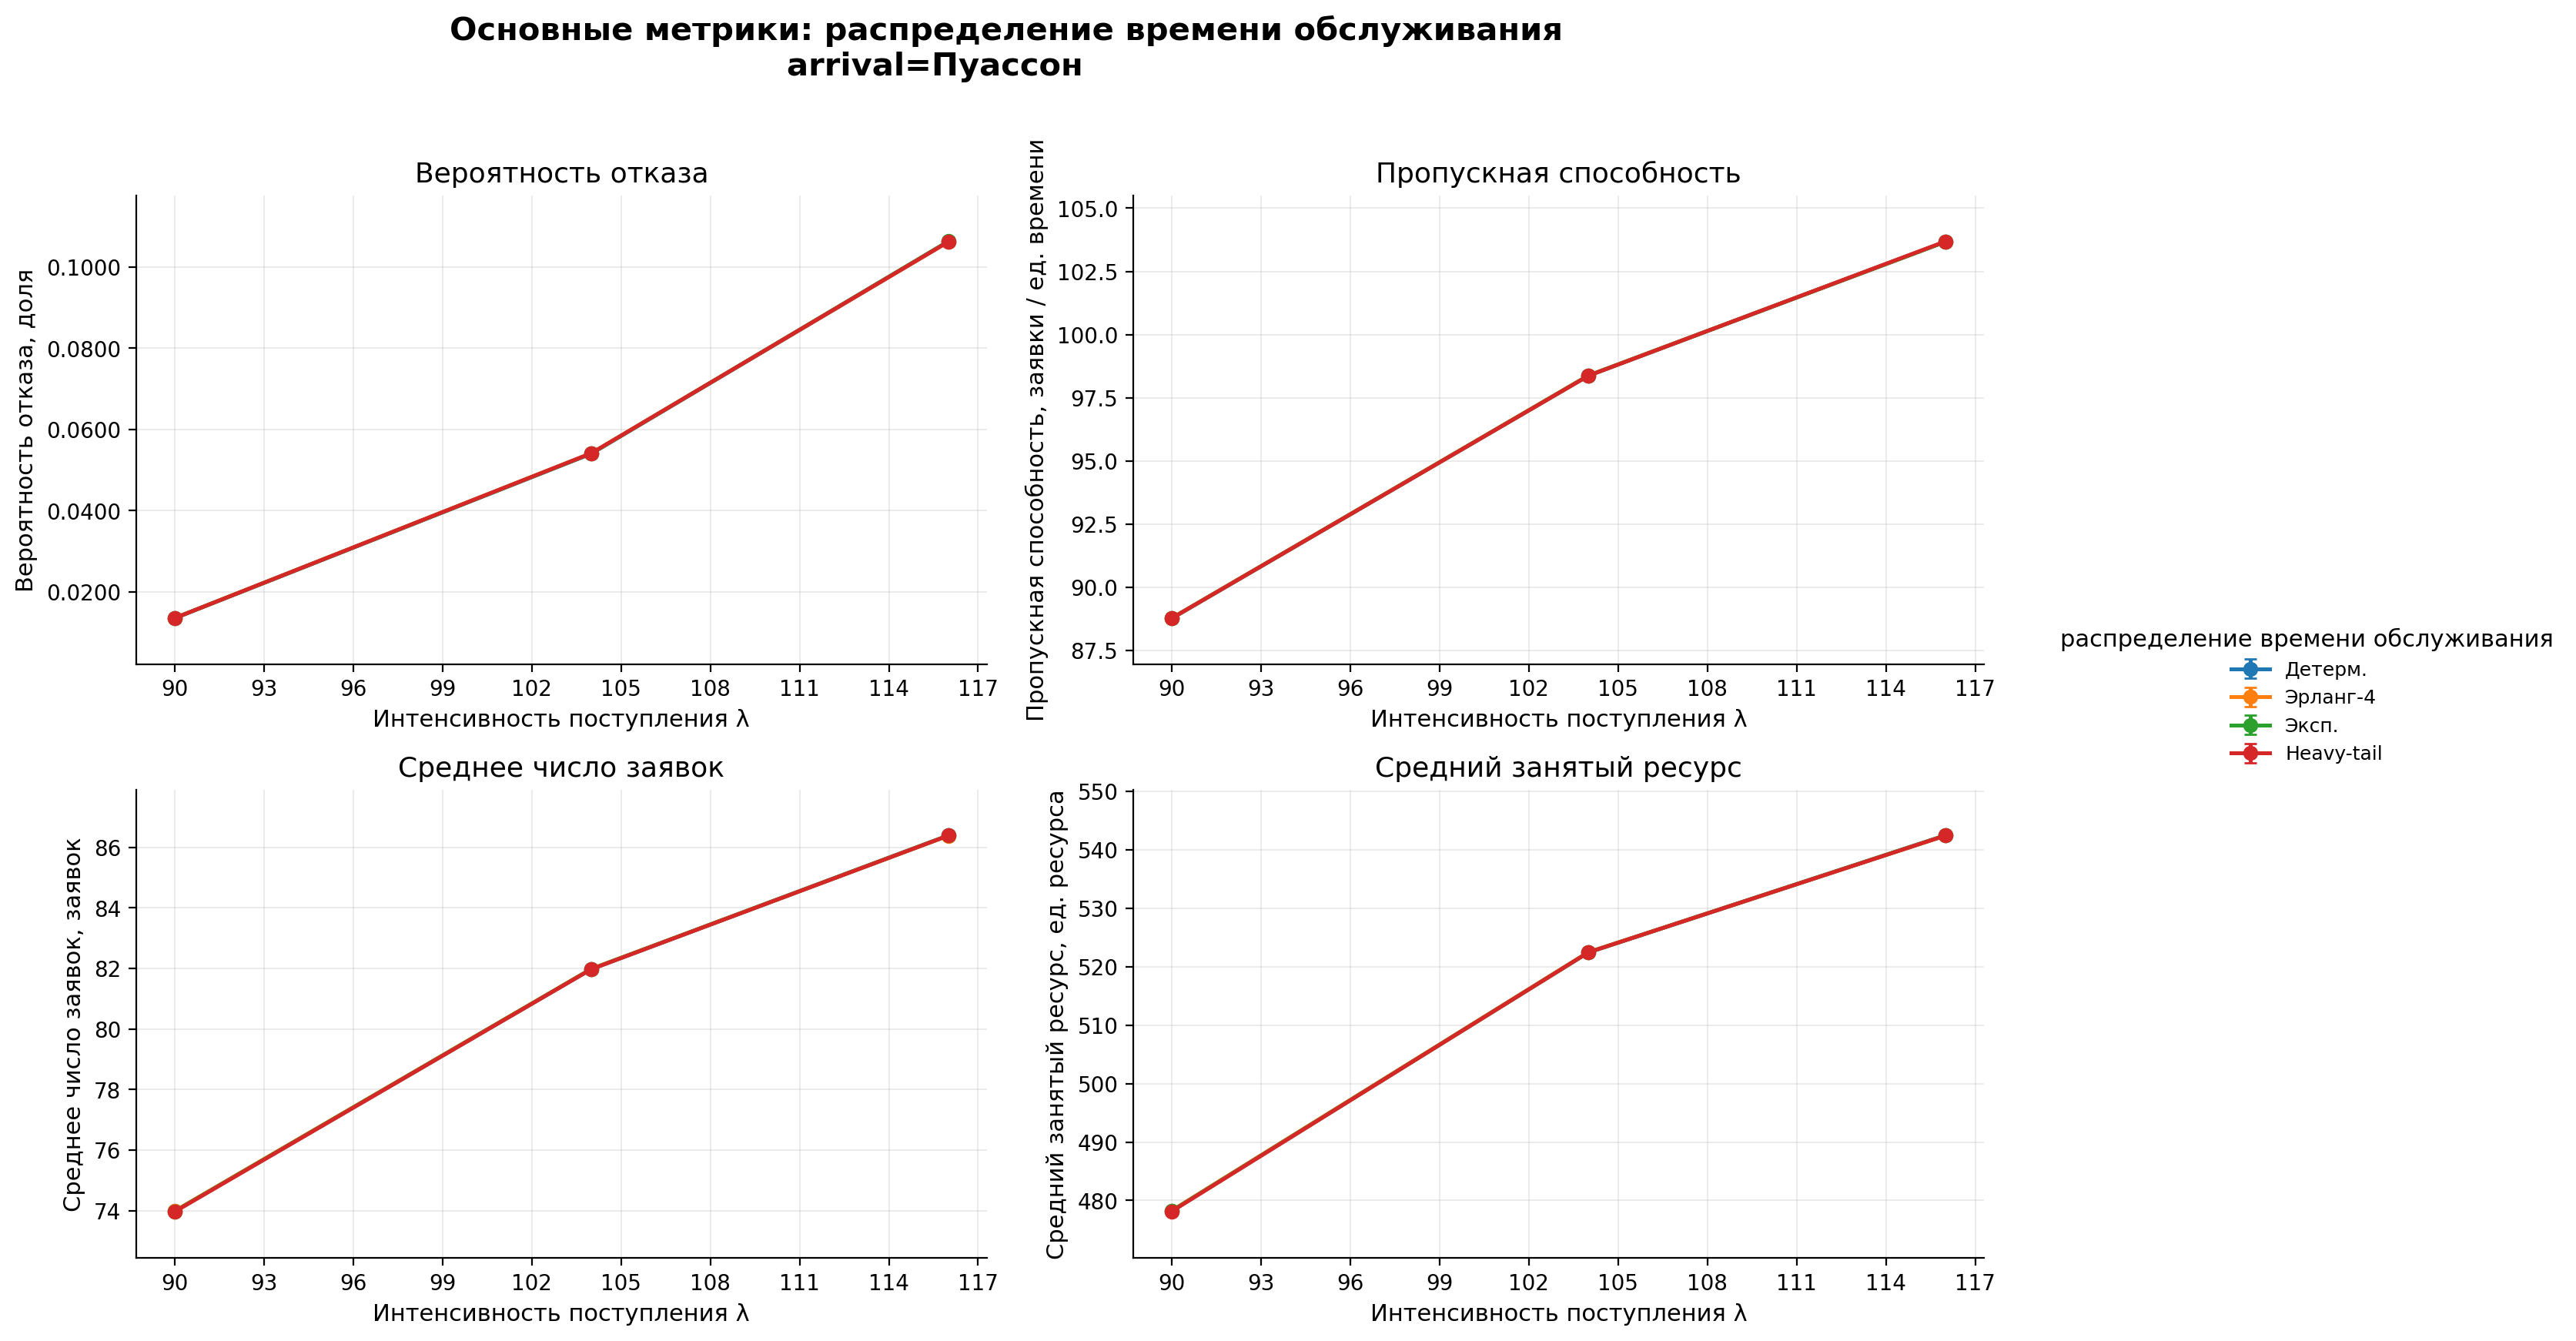
\includegraphics[width=0.95\textwidth]{workload_sensitivity_main_metrics_sigma-1p2}
    \caption{Основные показатели эффективности системы при различных распределениях времени обслуживания}
    \label{fig:workload_main_metrics}
\end{figure}

Анализ относительного смещения показателей относительно марковского экспоненциально распределенного базиса, представленные на рисунке~\ref{fig:workload_delta}, показывают, что девиации большинства метрик от не превышают долей процента.

\begin{figure}[H]
    \centering
    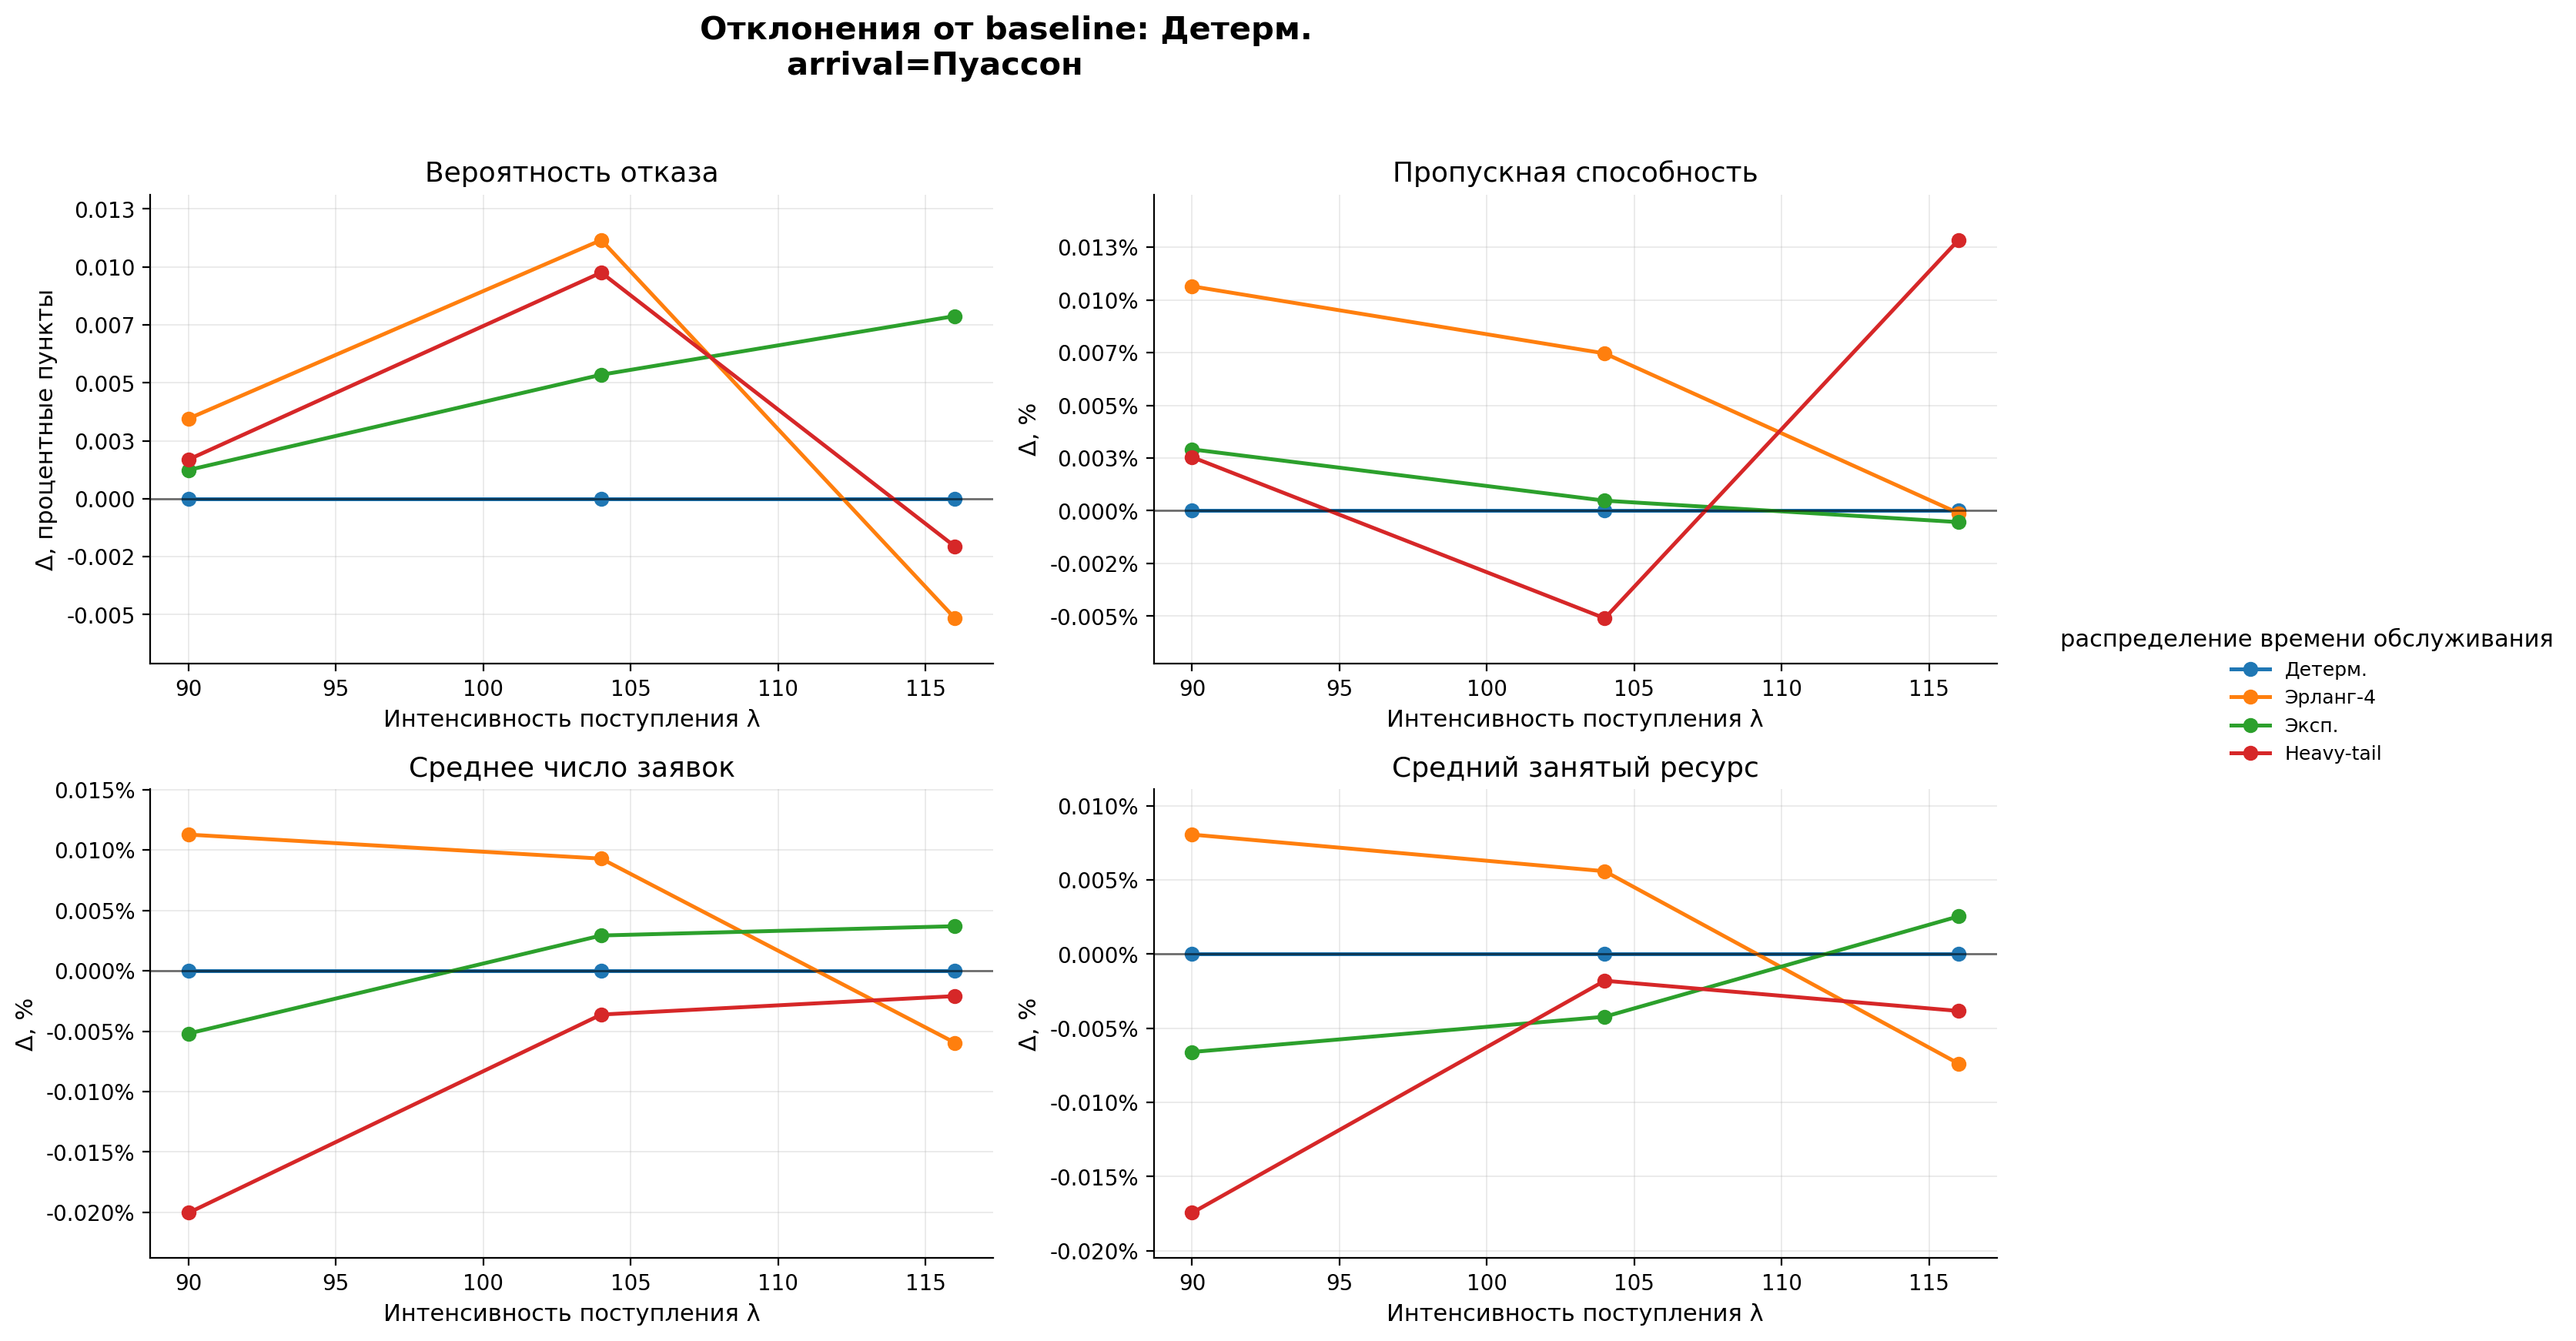
\includegraphics[width=0.85\textwidth]{workload_sensitivity_delta_from_baseline_sigma-1p2}
    \caption{Относительное отклонение метрик от базового распределения обслуживания}
    \label{fig:workload_delta}
\end{figure}

Эффект от изменения формы распределения времени обслуживания сопоставим с уровнем статистического шума метода Монте-Карло, как видно из диаграммами размаха на рисунке~\ref{fig:workload_boxplot}. Средние значения находятся практически на одной линии. 

\begin{figure}[H]
    \centering
    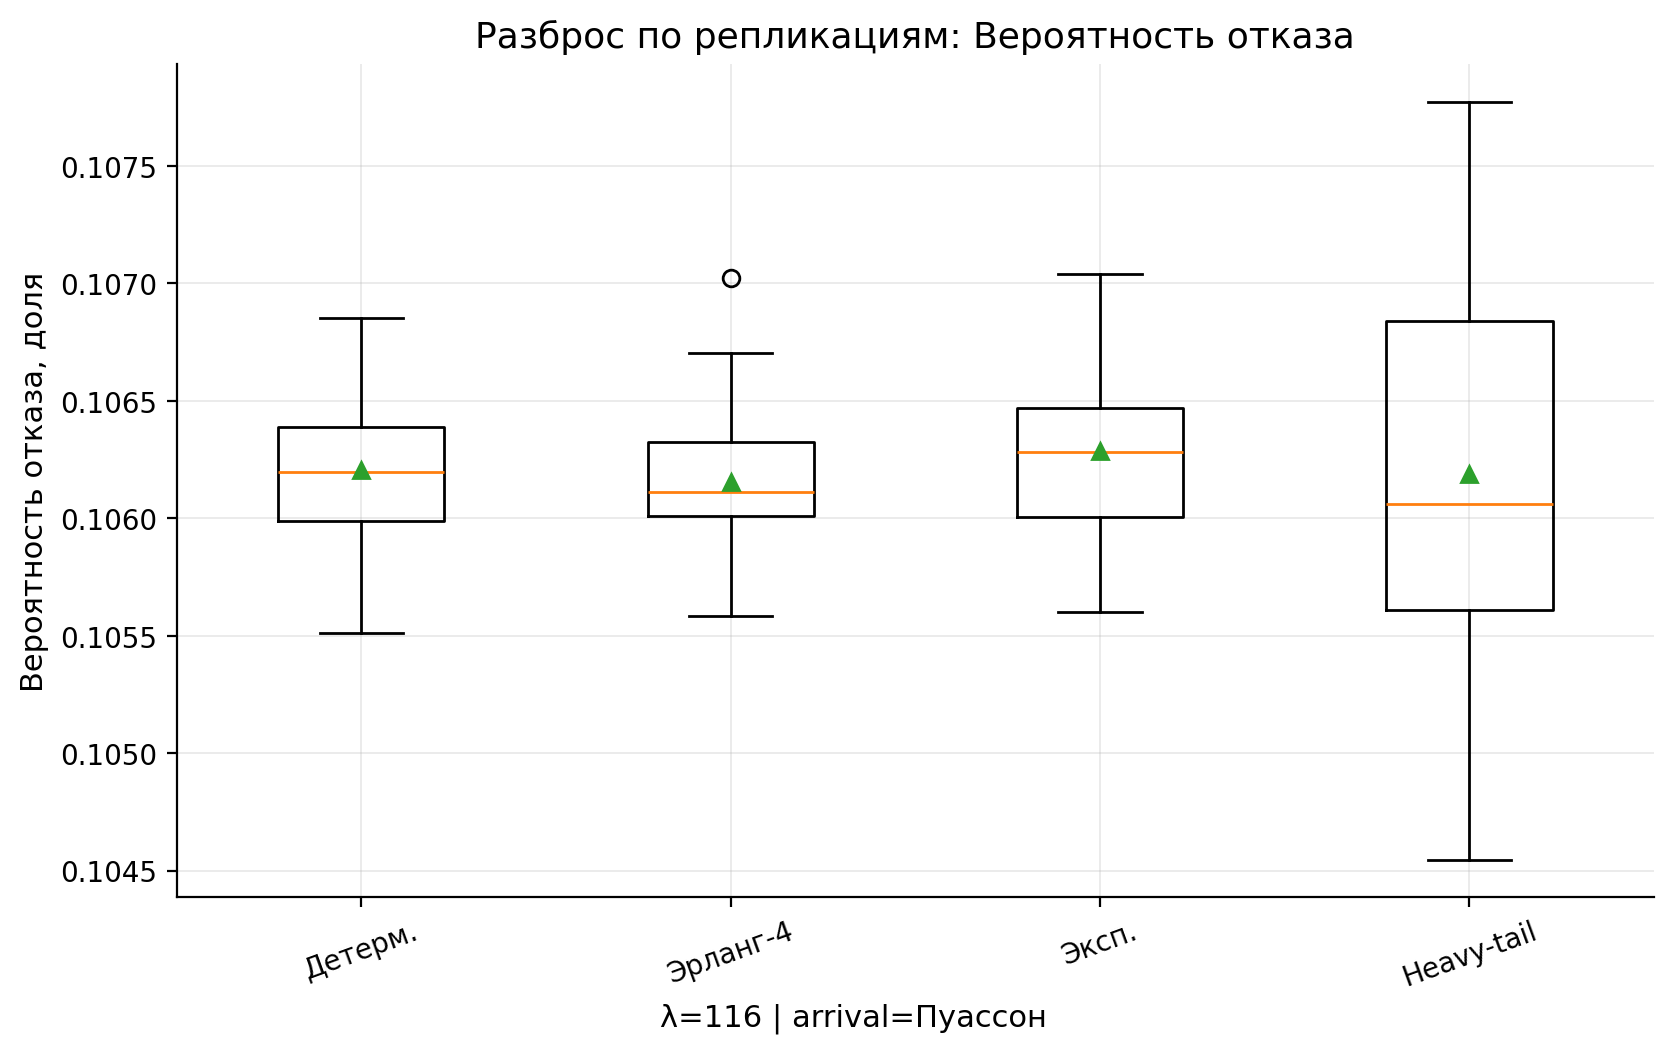
\includegraphics[width=0.85\textwidth]{workload_sensitivity_boxplot_loss_probability_sigma-1p2_lambda-116}
    \caption{Диаграмма размаха вероятности потери для различных типов обслуживания ($\lambda = 116$)}
    \label{fig:workload_boxplot}
\end{figure}

При этом межквартильные размахи (ширина «ящиков»), отражающие дисперсию результатов между независимыми репликациями, полностью перекрывают друг друга.

На рисунке~\ref{fig:workload_stationary} показана оценка стационарного распределения числа заявок в системе $\pi(k)$.

\begin{figure}[H]
    \centering
    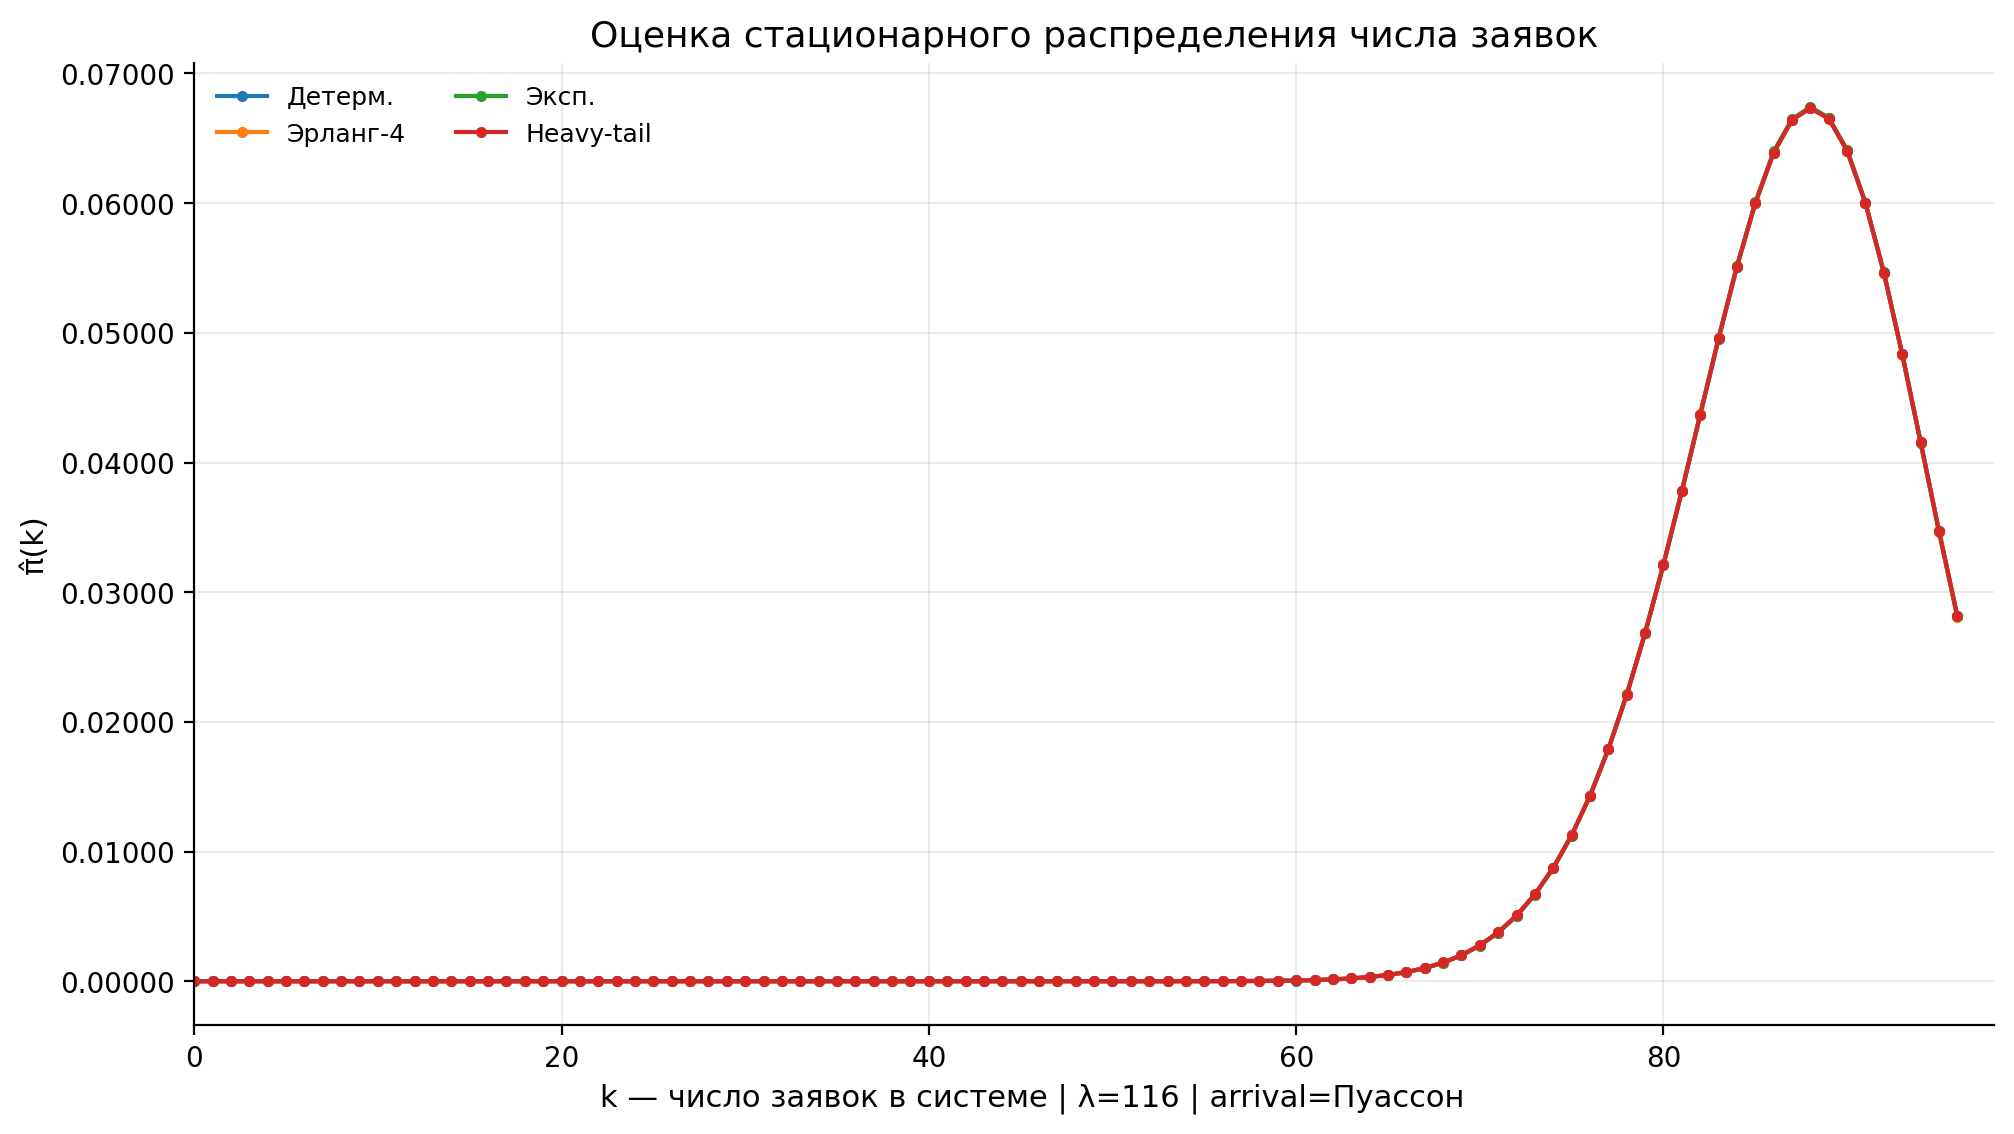
\includegraphics[width=0.95\textwidth]{workload_sensitivity_stationary_distribution_sigma-1p2_lambda-116}
    \caption{Оценка стационарного распределения вероятностей состояний $\pi(k)$ ($\lambda = 116$)}
    \label{fig:workload_stationary}
\end{figure}

Кривые вероятностей состояний для детерминированного, экспоненциального, эрланговского и гиперэкспоненциального законов обслуживания совпадают на всем диапазоне возможных состояний.

\subsection*{Выводы по разделу}
При марковском (пуассоновском) входящем потоке в исследуемой ресурсной системе чувствительность к закону распределения времени работы заявки практически отсутствует. Все зафиксированные расхождения не превышают долей процента и полностью объясняются дисперсией метода Монте-Карло. Полученный результат согласуется с классическим свойством инвариантности  стационарного распределения\cite{sevastyanov1957_ergodic_refusals,burman1981_insensitivity,sopin2018_insensitivity}. 

Таким образом, для данного режима работы подтверждена возможность использования простейших экспоненциальных аппроксимаций $M/M/N/R$ без потери точности моделирования \cite{dudin2025_random_environment}.
% Главная идея раздела:
% workload сам по себе почти не меняет стационарные характеристики,
% особенно при пуассоновском входе.
%
% Это не слабый результат, а важный результат:
% он показывает, что модель ведёт себя согласно известной инвариантности.
%
% Здесь лучше не писать "результатов нет".
% Писать надо так:
% "наблюдается слабая чувствительность", "эффект сопоставим с шумом Монте-Карло",
% "результат согласуется с инвариантностью".

\section{Чувствительность к типу входящего потока}
\label{sec:arrival_sensitivity_results}

В данном разделе анализируется влияние типа входящего потока на показатели эффективности ресурсной системы с потерями\cite{paxson_floyd_1995_poisson_failure,leland_taqqu_willinger_wilson_1994_selfsimilar,vishnevskii_dudin_correlated_arrivals_2017}. Рассматриваются следующие типы входящего потока$\{\text{Poisson}, \text{Erlang-2}, \text{Erlang-4}, \text{HyperExp-2}\}$, при фиксированном детерминированном распределении времени работы.

Во всех сценариях данного раздела выполняется условие $\mathbb{E}[A] = \frac{1}{\lambda},$
где $A$ --- случайный межприходный интервал. Базовым сценарием для сравнения выбран пуассоновский поток $a_0 = \text{Poisson}$.

На рисунке~\ref{fig:arrival_main_metrics} представлены основные показатели эффективности системы при различных типах входящего потока и уровнях интенсивности $\lambda$.

\begin{figure}[H]
    \centering
    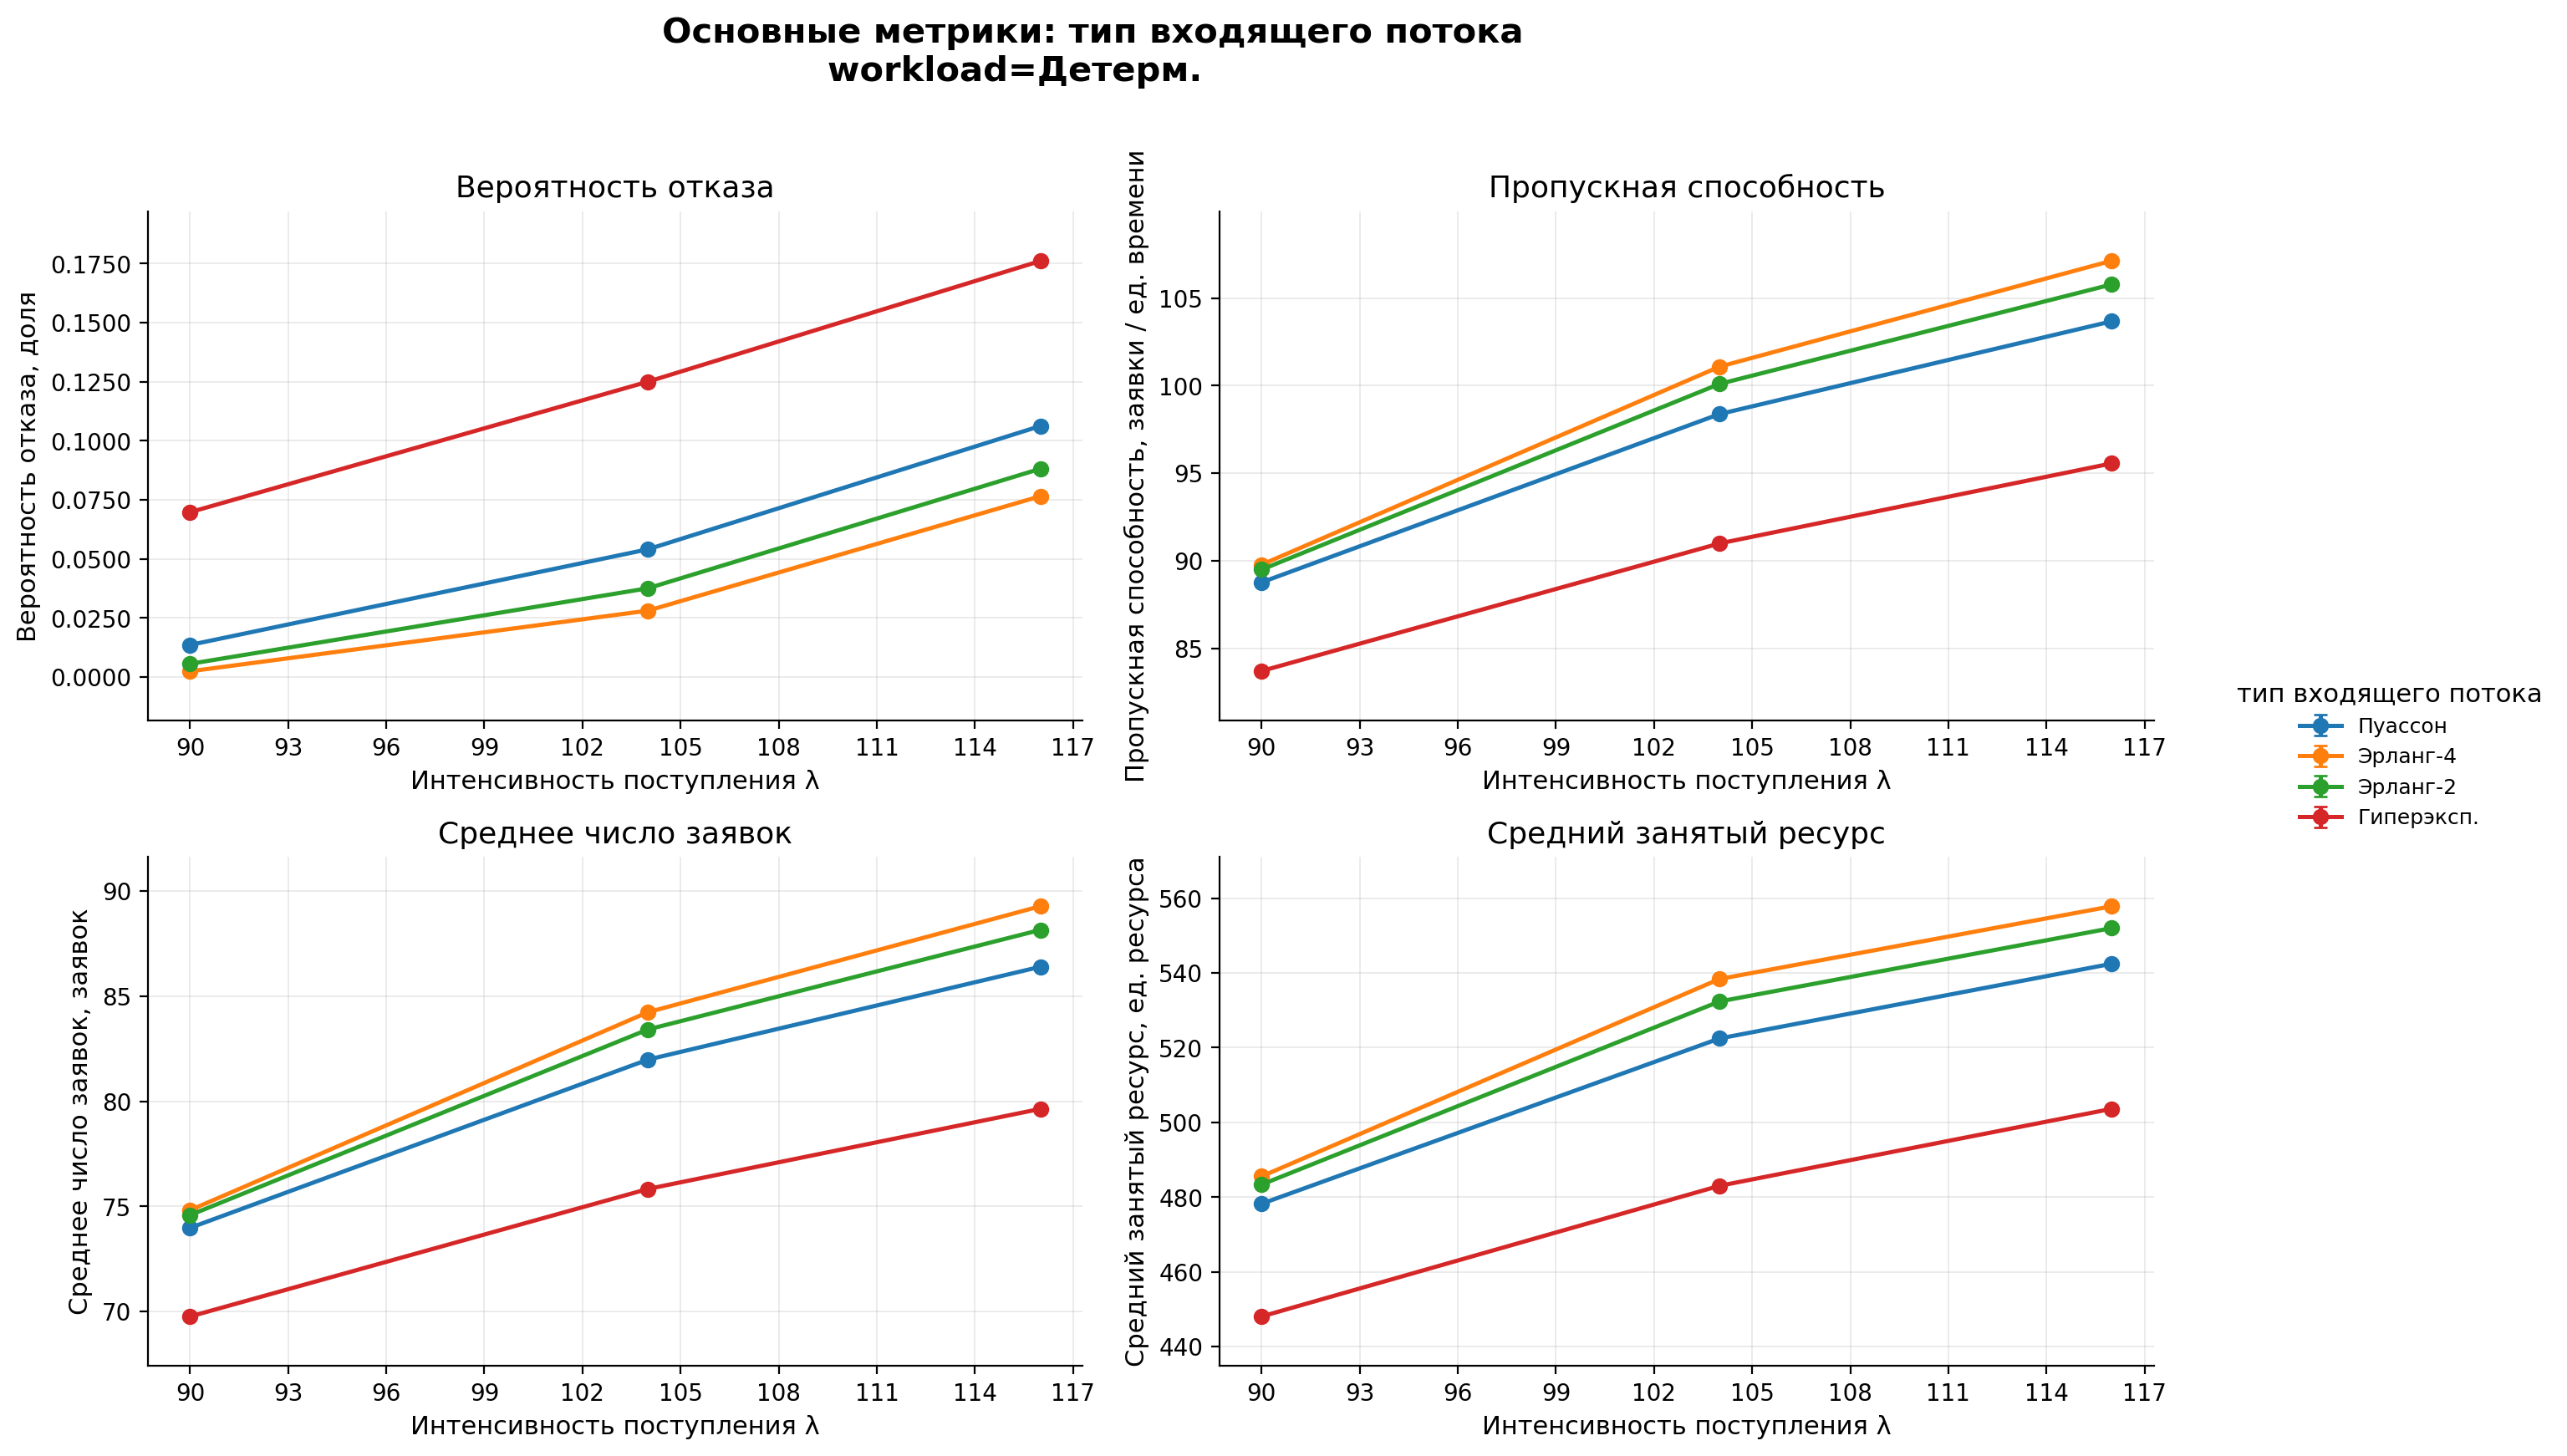
\includegraphics[width=0.95\textwidth]{images/arrival_sensitivity_main_metrics_sigma-1p2.png}
    \caption{Основные показатели эффективности системы при различных типах входящего потока}
    \label{fig:arrival_main_metrics}
\end{figure}

При увеличении $\lambda$ вероятность отказа возрастает; темп роста различается для разных распределений. Наименьшие значения вероятности отказа наблюдаются для регулярных эрланговских потоков, а наибольшие --- для гиперэкспоненциального потока.


На рисунке~\ref{fig:arrival_loss_bars} отдельно показана вероятность отказа по уровням интенсивности $\lambda$.

\begin{figure}[H]
    \centering
    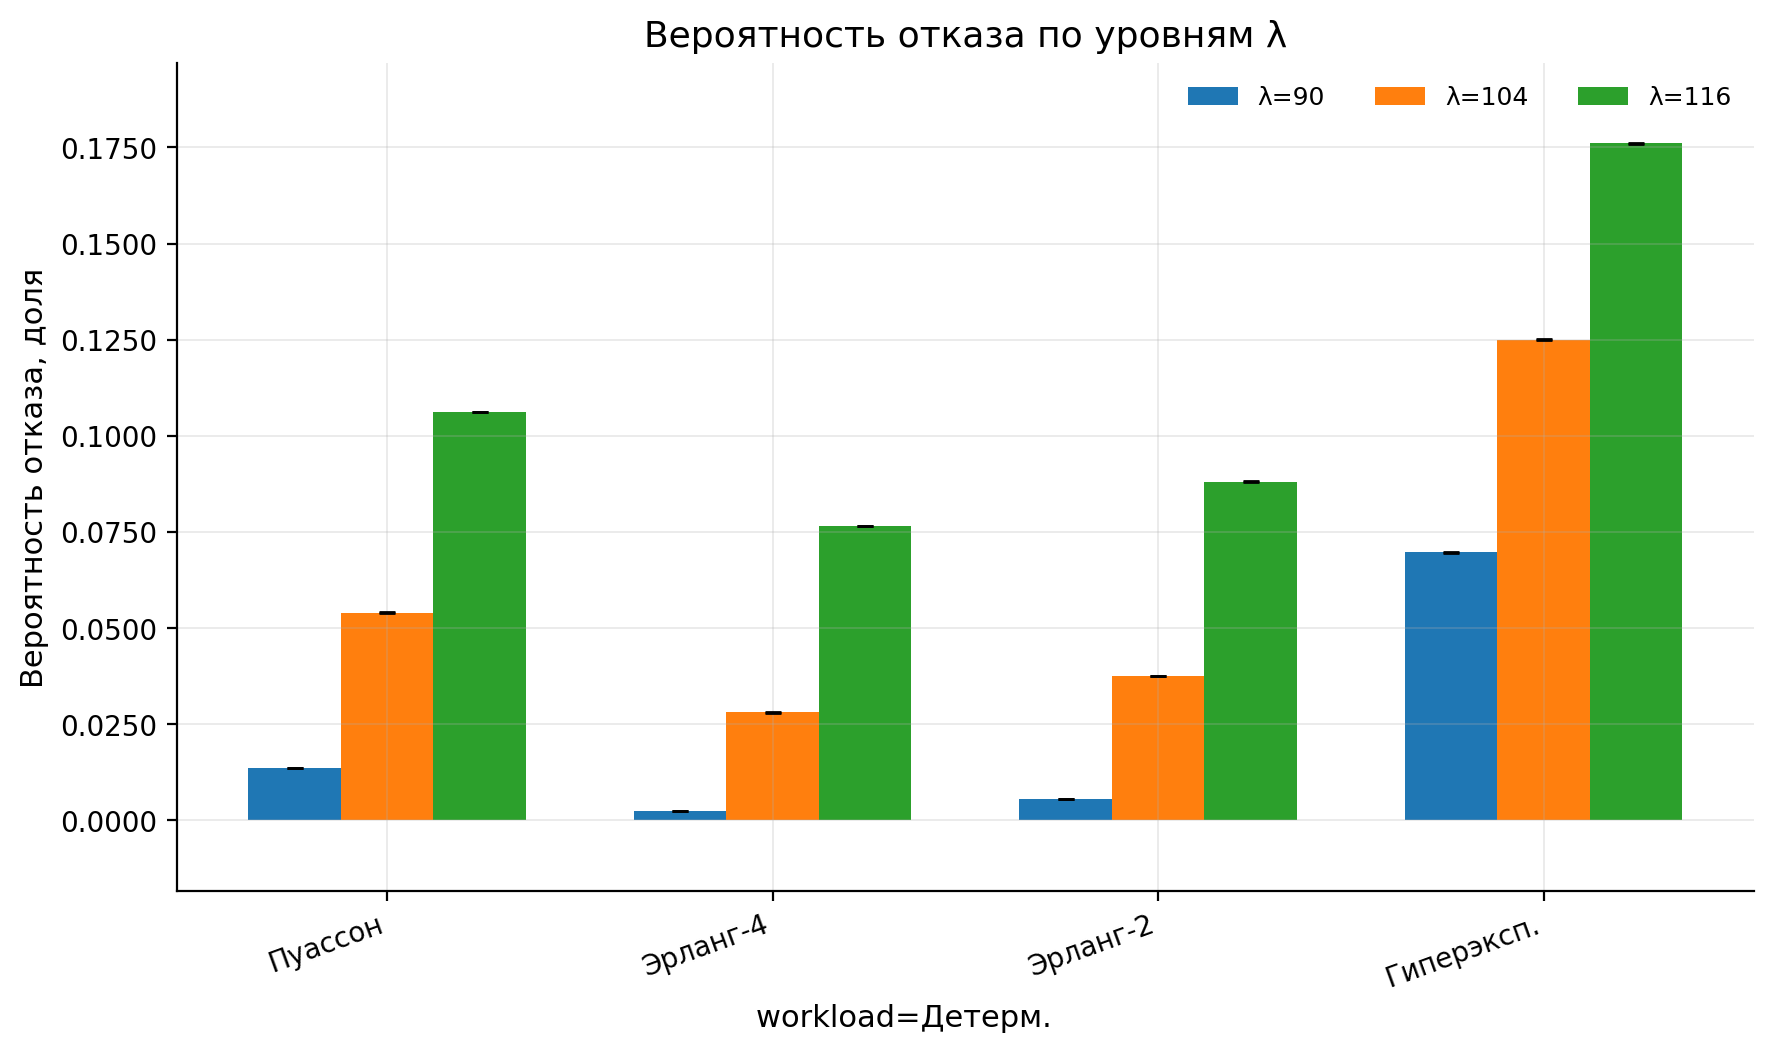
\includegraphics[width=0.90\textwidth]{images/arrival_sensitivity_loss_probability_bars_by_lambda_sigma-1p2.png}
    \caption{Вероятность отказа при различных типах входящего потока и уровнях $\lambda$}
    \label{fig:arrival_loss_bars}
\end{figure}

Чем больше $\lambda$ тем более выраженным становится различие между различными распределениями входящего потока. Гиперэкспоненциальный поток даёт максимальную вероятность отказа, а поток Эрланга четвёртого порядка остаётся наиболее благоприятным.


Для проверки устойчивости полученных различий были построены диаграммы размаха по независимым репликациям\cite{tukey1977_exploratory_data_analysis}. Ниже приведён разброс вероятности отказа при $\lambda=116$.

\begin{figure}[H]
    \centering
    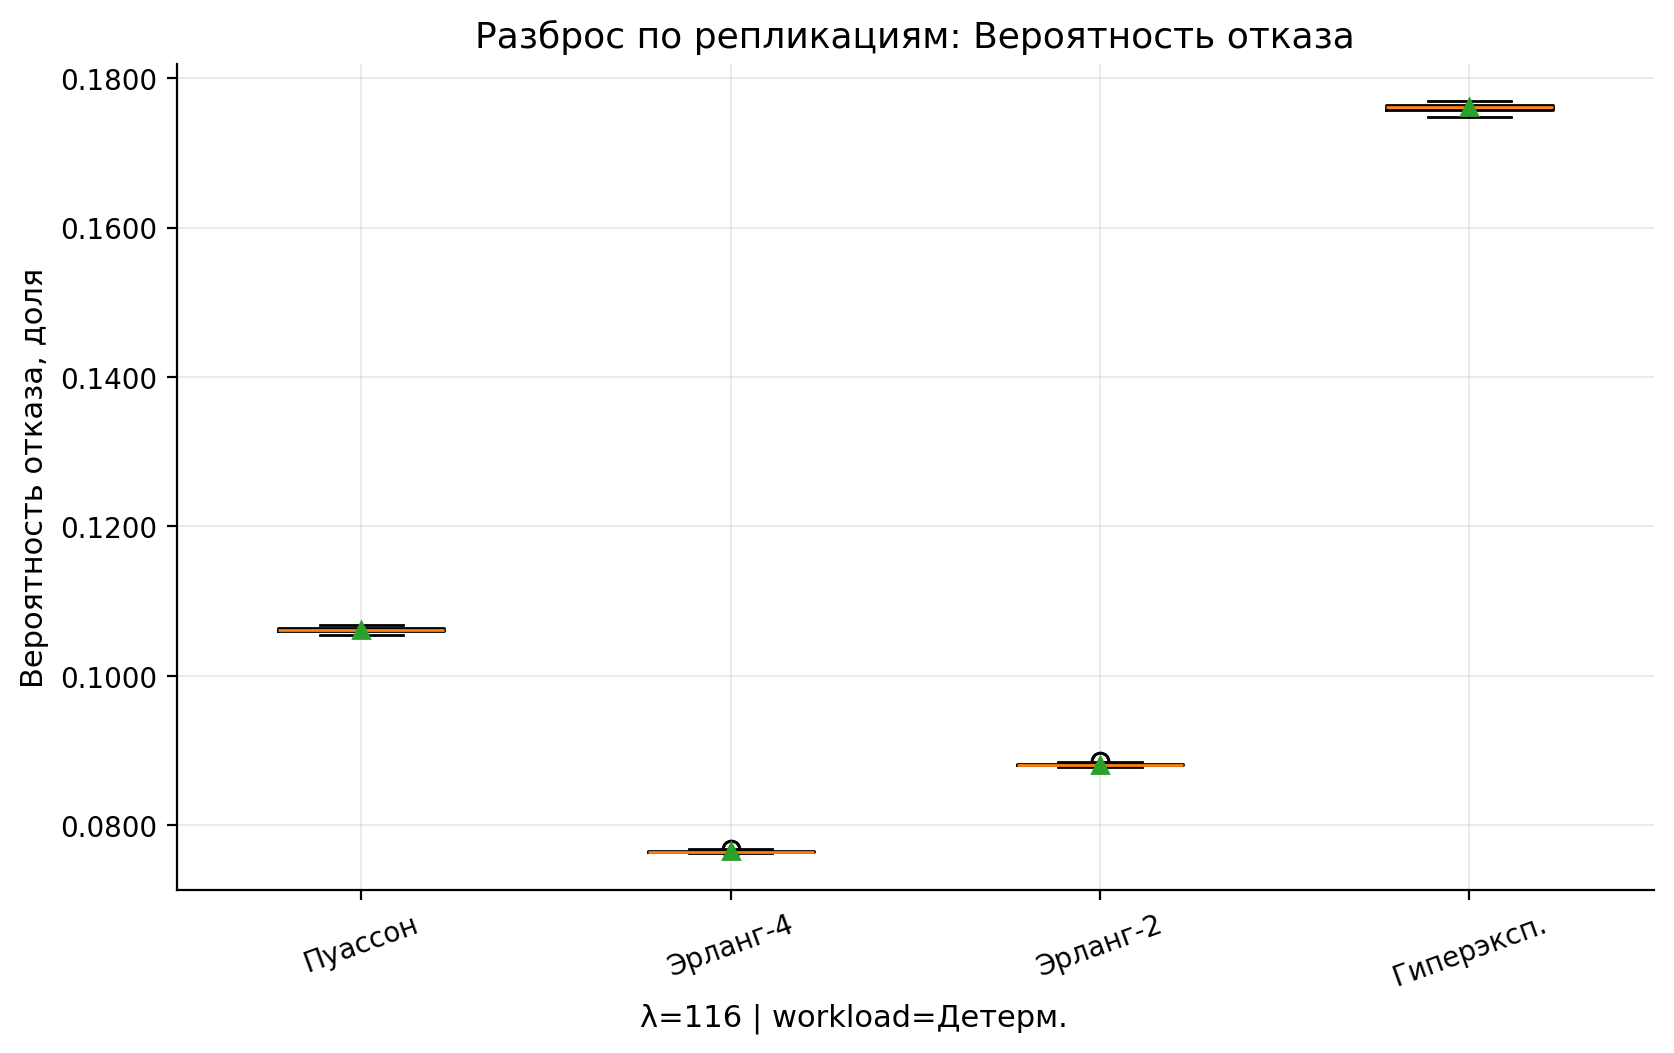
\includegraphics[width=0.90\textwidth]{images/arrival_sensitivity_boxplot_loss_probability_sigma-1p2_lambda-116.png}
    \caption{Разброс вероятности отказа по репликациям при $\lambda=116$}
    \label{fig:arrival_boxplot_loss}
\end{figure}

Видно, что межсценарные различия значительно превышают внутрисценарный разброс по репликациям. Наблюдаемая чувствительность к типу входящего потока не является следствием шума Монте-Карло\cite{law2015_simulation_modeling,welch1983_statistical_analysis_simulation}. В отличие от результатов по распределению workload, здесь различия между сценариями статистически выражены.

На рисунке~\ref{fig:arrival_stationary_dist} показано исследование $\pi(k)$ при $\lambda = 116$.

\begin{figure}[H]
    \centering
    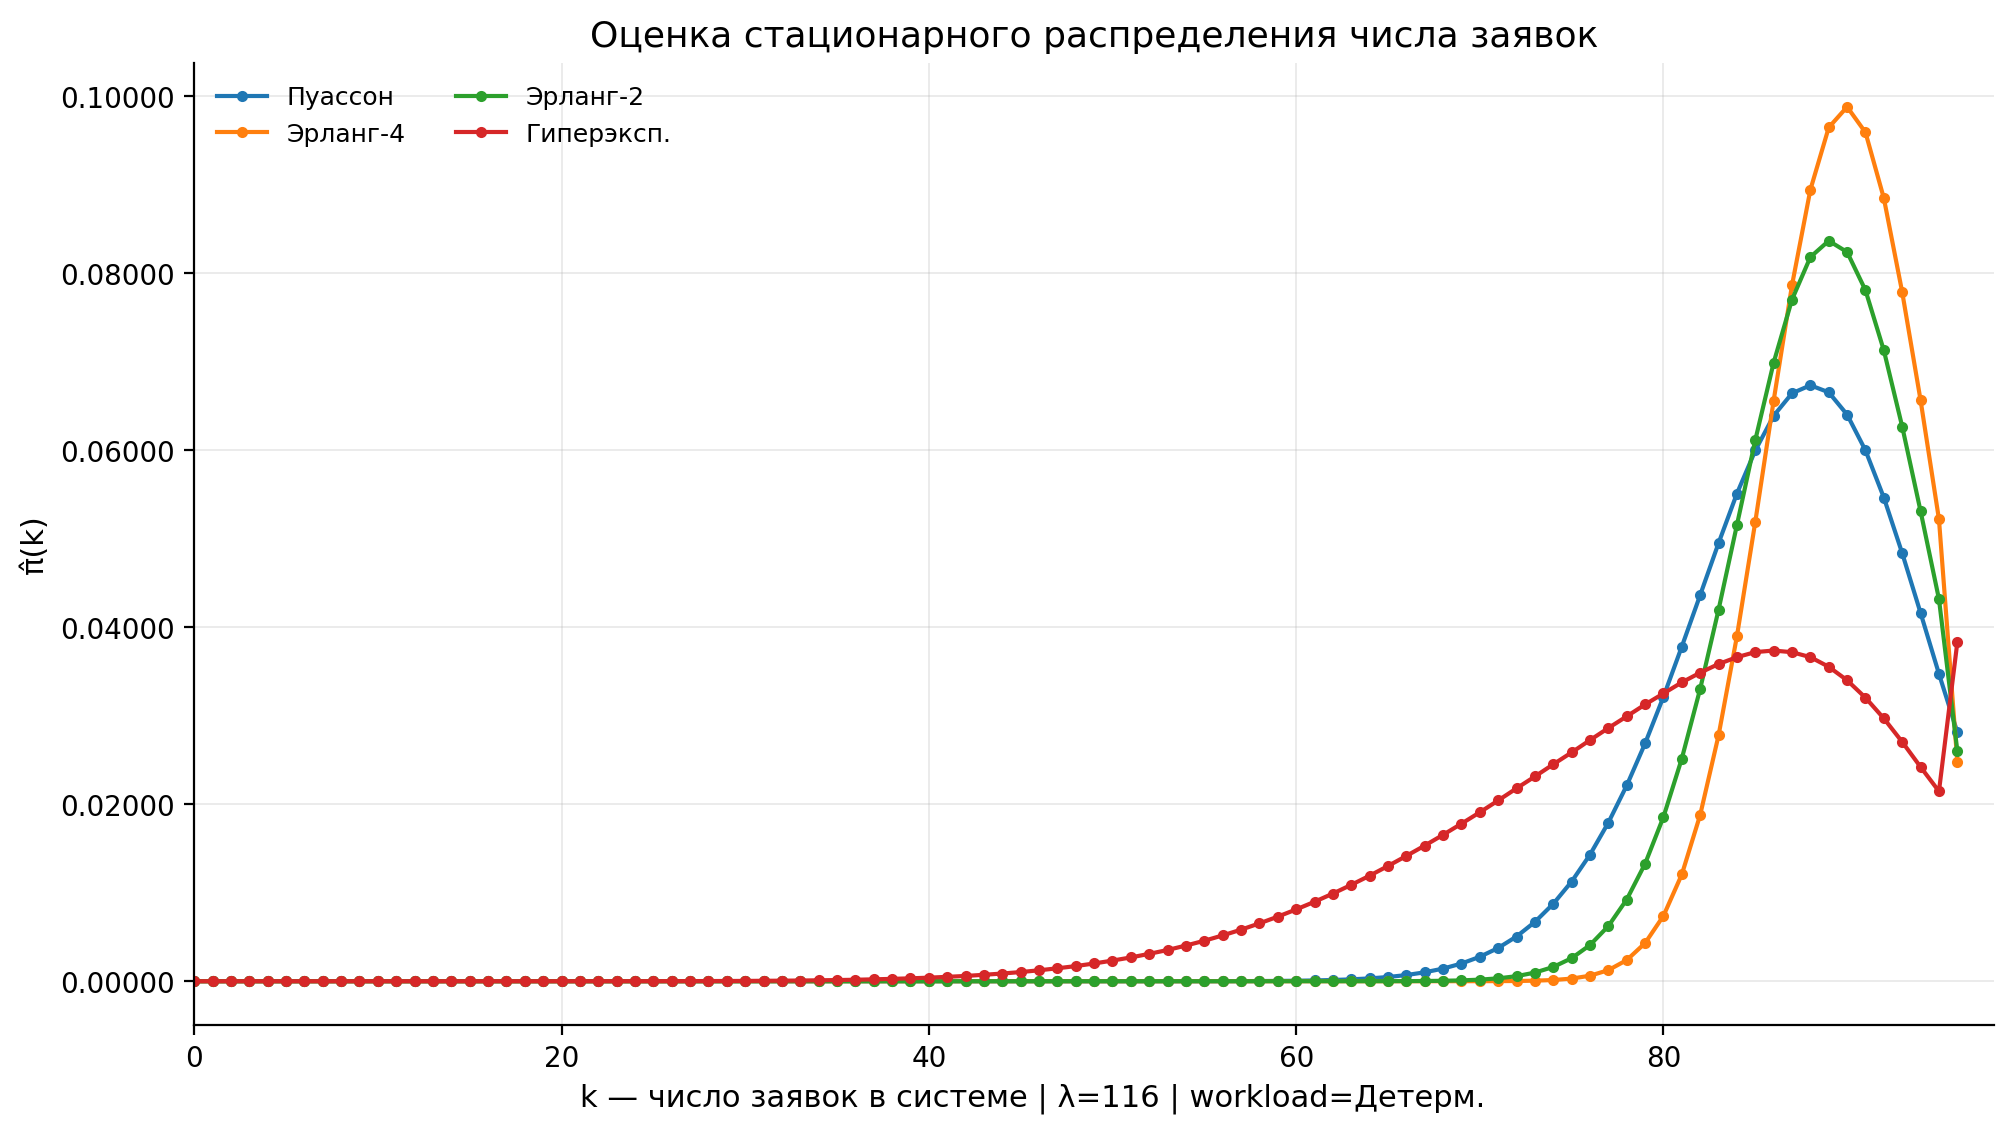
\includegraphics[width=0.95\textwidth]{images/arrival_sensitivity_stationary_distribution_sigma-1p2_lambda-116.png}
    \caption{Стационарное распределение числа заявок в системе $\pi(k)$ при различных типах входящего потока ($\lambda = 116$)}
    \label{fig:arrival_stationary_dist}
\end{figure}

Кривые на графике сильно варьируются, для регулярных потоков распределение смещено в сторону больших значений $k$. При гиперэкспоненциальном входящем потоке распределение $\pi(k)$ более пологое, но растет ближе к левому краю из-за редких приходов больших пачек заявок.

Дополнительно была построена оценка хвоста стационарного распределения числа заявок в системе~\ref{fig:arrival_stationary_tail}.

\begin{figure}[H]
    \centering
    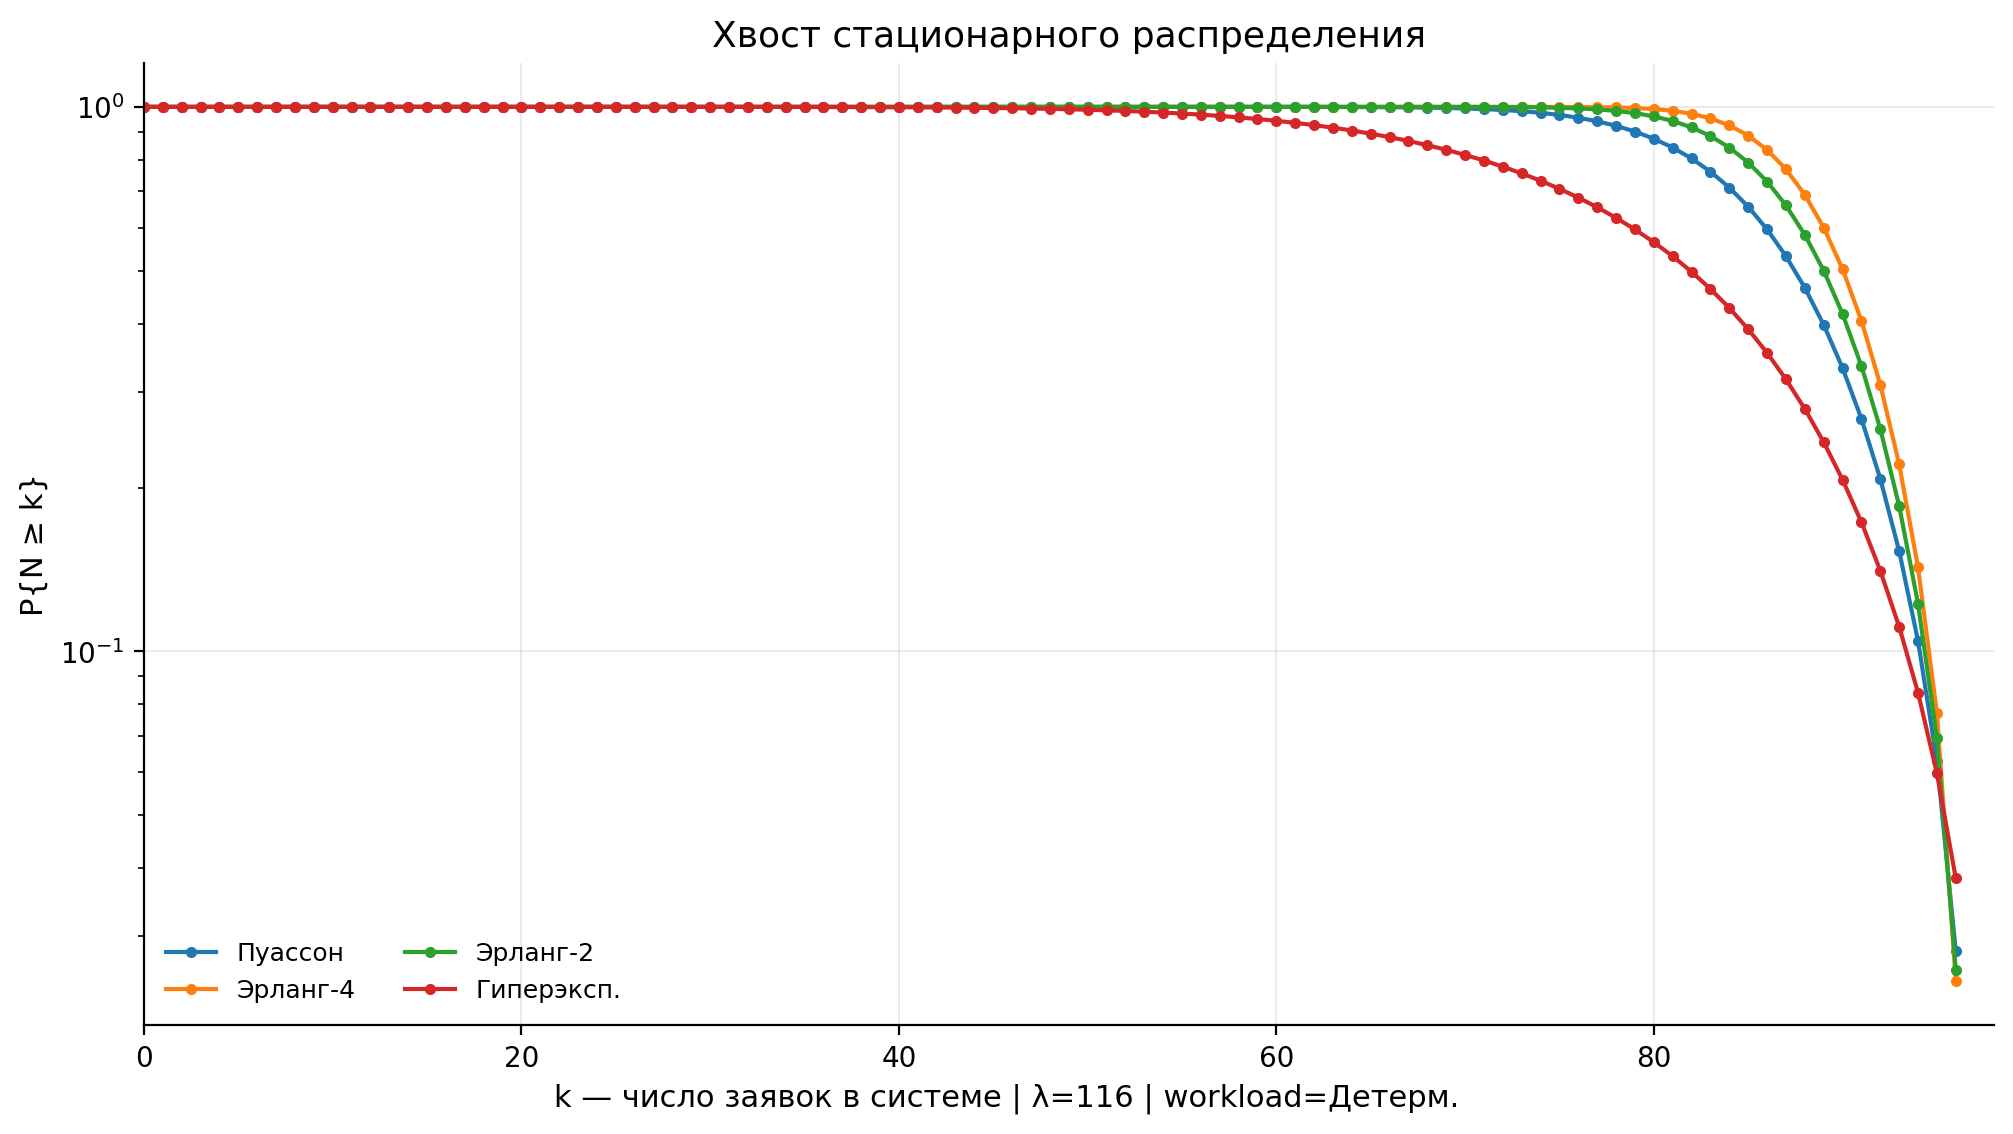
\includegraphics[width=0.95\textwidth]{images/arrival_sensitivity_stationary_tail_sigma-1p2_lambda-116.png}
    \caption{Хвост стационарного распределения числа заявок в системе при $\lambda=116$}
    \label{fig:arrival_stationary_tail}
\end{figure}

Хвостовое распределение подтверждает различие режимов заполнения системы. Для регулярных эрланговских потоков распределение держится на высоких (много заявок в системе) устойчивых значениях - загрузка равномерная. У гиперэкспоненциального входящего потока хвост убывает медленнее - высокая вероятность состояний с высокой занятостью системы, множество отказов по ресурсу $R$.

\subsection*{Выводы по разделу}

Тип входящего потока является ключевым факторов чувствительности ресурсной системы с потерями\cite{paxson_floyd_1995_poisson_failure,vishnevskii_dudin_correlated_arrivals_2017}. При одинаковом $\lambda$ различные распределения межприходных интервалов приводят к принципиально разной вероятности отказа, пропускной способности и средней занятости.

Регулярные потоки Эрланга уменьшают вероятность отказа, а гиперэкспоненциальный поток увеличивает вероятность отказа из-за локальных перегрузок. 

% Главная идея:
% Это основной результат главы.
% При одинаковой средней интенсивности lambda разные распределения межприходных интервалов
% дают заметно разные p_loss, throughput, mean_num_jobs и mean_occupied_resource.
%
% Особенно важно:
% Erlang-потоки более регулярные, HyperExp-поток более bursty.
% Поэтому сравнение идет не по среднему, а по вариативности межприходных интервалов.

\section{Совместное влияние распределения обслуживания и входного потока}
\label{sec:combined_sensitivity_results}

В данном разделе анализируется полный набор сценариев, в котором одновременно варьируются тип входящего потока $a$, распределение объёма работы заявки $\omega$ и интенсивность поступления $\lambda$.

Каждый сценарий можно записать в виде
$$
s = (a, \omega, \lambda, \mu, N, R, F_D),
$$
где $a$ --- тип входящего потока, $\omega$ --- тип распределения workload, $\lambda$ --- средняя интенсивность поступления, $\mu$ --- скорость обслуживания, $N$ --- число обслуживающих каналов, $R$ --- общий объём ресурса, $F_D$ --- распределение ресурсного требования заявки. 

В рамках проводимых экспериментов зафиксированы $N = 96, R = 590, \mu = 1.2, F_D$ заданы таблично, следовательно каждый экспериментальный сценарий однозначно задается сокращенным вектором $s' = (a, \omega, \lambda)$. Базовым сценарием является детерминированный workload и пуассоновский входящим потоком $
s'_0(\lambda) = (\text{Poisson}, \text{Deterministic}, \lambda)$.

Взаимное влияние этих переменных на показатели системы удобно отражать в тепловых картах, так, например,  на рисунке ~\ref{fig:combined_loss_matrix} показана веротяность отказа.

\begin{figure}[H]
    \centering
    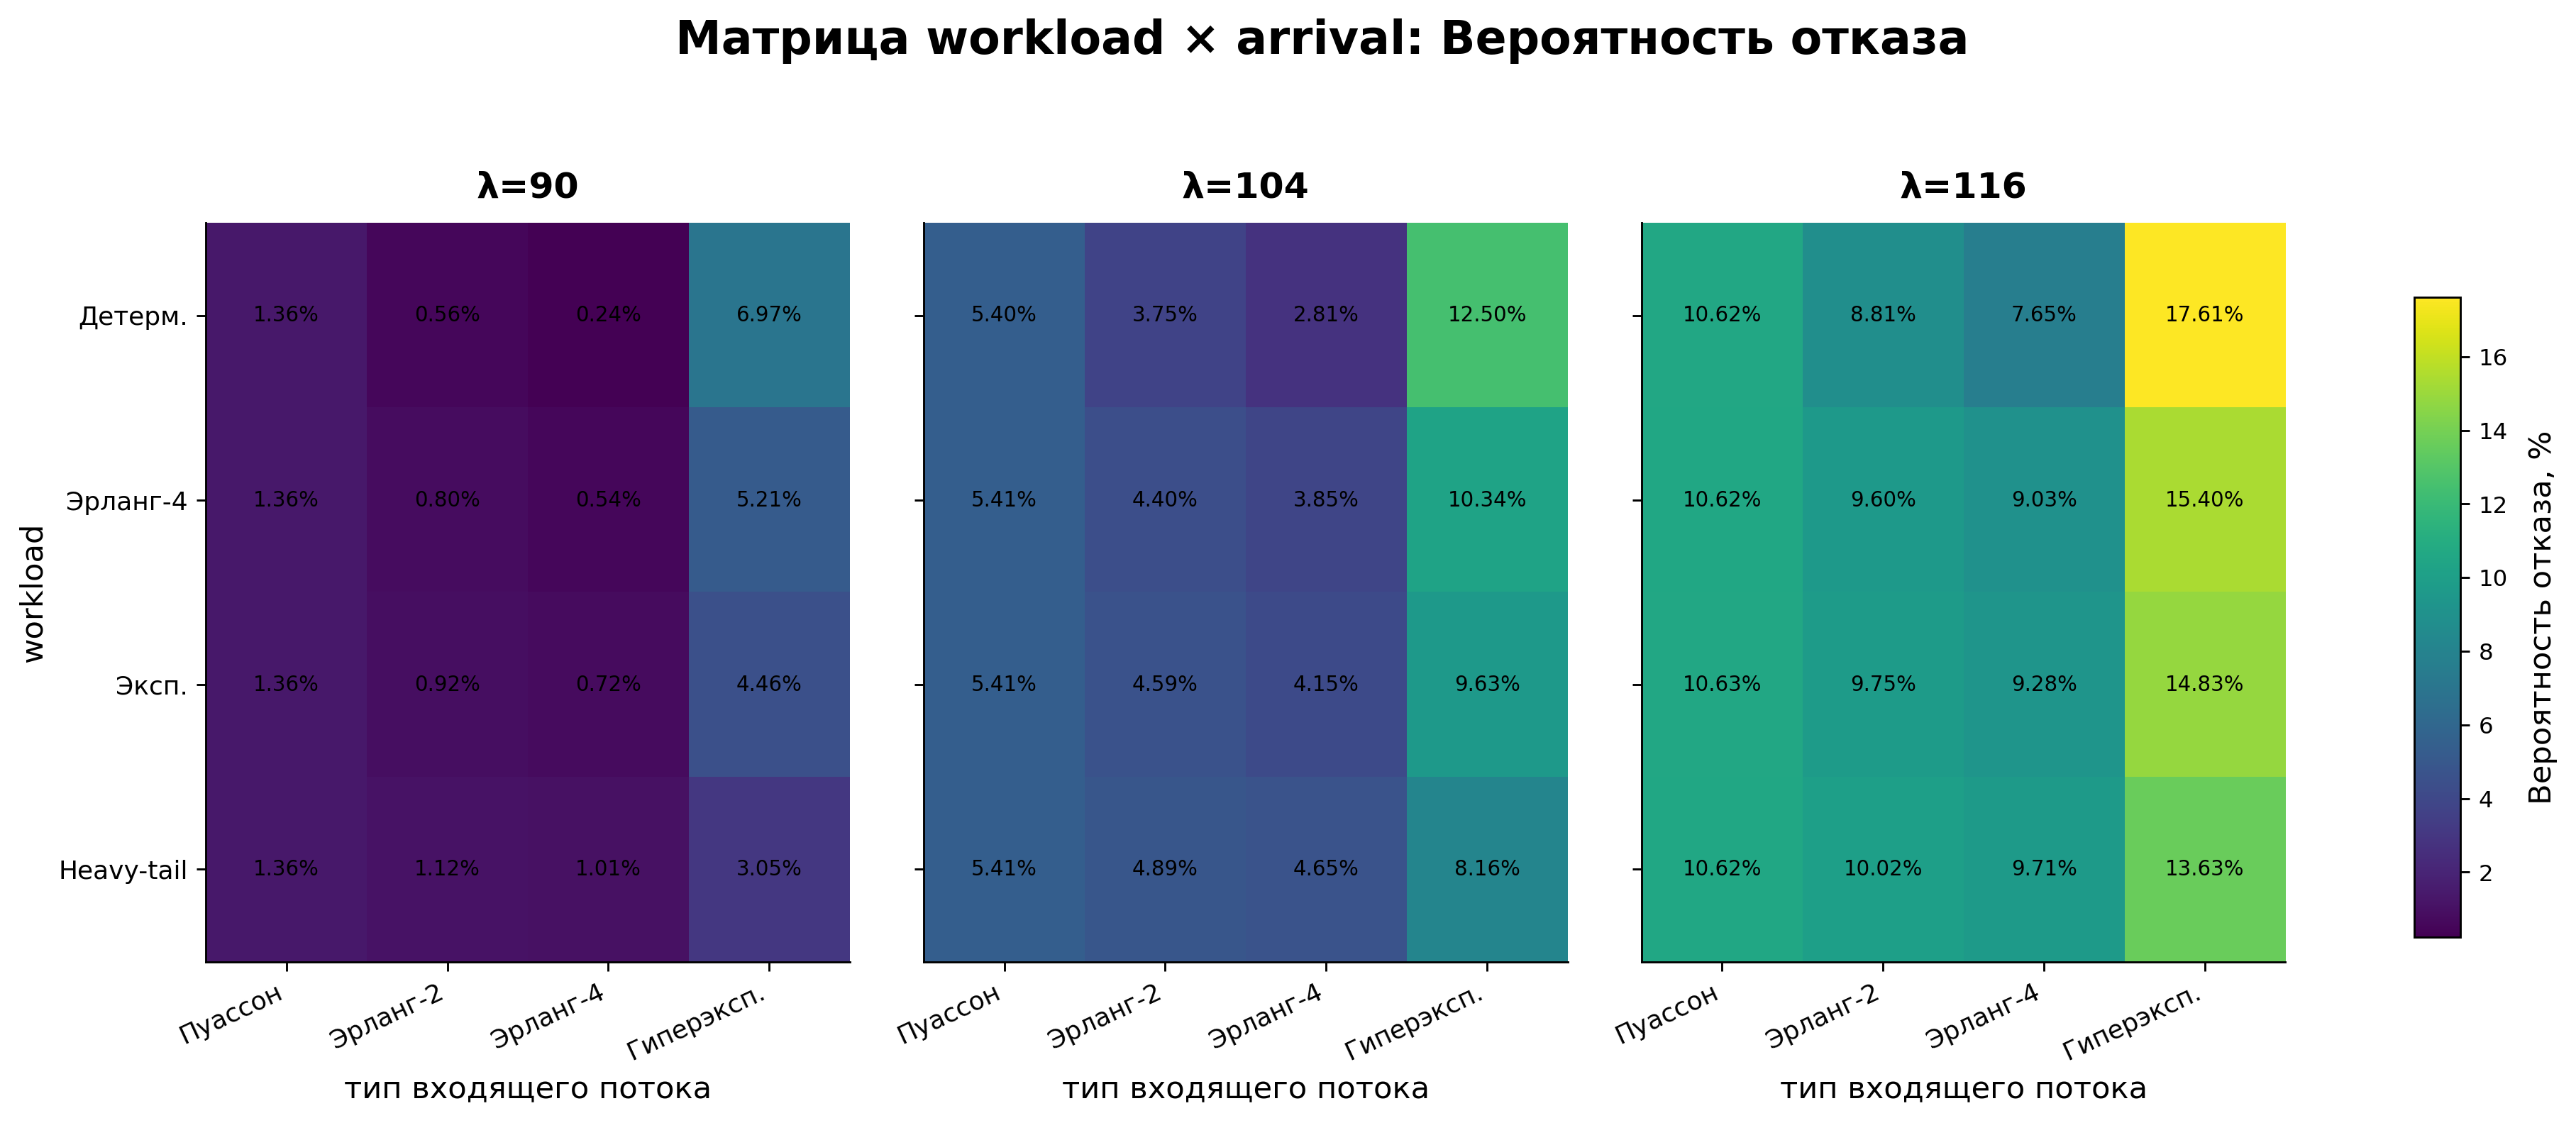
\includegraphics[width=0.98\textwidth]{images/01_heatmap_workload_arrival_loss_probability_sigma-1p2.png}
    \caption{Матрица workload $\times$ arrival для вероятности отказа}
    \label{fig:combined_loss_matrix}
\end{figure}


% !!!Переменные без крышки - теоретические значения. Переменные с крышкой - эмпирическая оценка.
% m - просто метрика

При пуассоновском входящем потоке $P_{\text{loss}}$ практически не зависит от распределения workload, как было ранее установлено в ~\ref{sec:workload_sensitivity_results}. При $c_A^2 = 1$, изменение $c_B^2$ практически не меняет вероятность отказа. Например, при $\lambda=116$ для всех четырёх workload расхождения вероятности отказа находятся на уровне $0.01$ процентного пункта: $10.62\%,\quad 10.62\%,\quad 10.63\%,\quad 10.62\%$. 
Это подтверждает инвариантность РСМО относительно распределения времени обслуживания при пуассоновском входе.

При непуассоновских входящих потоках инвариантность по распределению workload нарушается\cite{paxson_floyd_1995_poisson_failure,vishnevskii_dudin_correlated_arrivals_2017}, причём знак эффекта зависит от вариативности входящего потока. Для регулярных потоков Эрланга увеличение вариативности workload повышает вероятность отказа, а для гиперэкспоненциального входа, наоборот, снижает её; выполняется следующий порядок квадратов коэффициентов вариации:
$$
c_A^2(\text{Erlang-4}) < c_A^2(\text{Erlang-2}) < c_A^2(\text{Poisson}) < c_A^2(\text{HyperExp}),
$$
где
$$
\begin{aligned}
    c_A^2(\text{Erlang-4}) &= 0.25, & c_A^2(\text{Erlang-2}) &= 0.5, \\
    c_A^2(\text{Poisson}) &= 1, & c_A^2(\text{HyperExp}) &> 1.
\end{aligned}
$$

Для регулярных входящих потоков наблюдается наименьшая вероятность отказа, но чем выше вариативность workload, тем больше будет вероятность отказа. При $\lambda=116$ и входящем потоке Erlang-4 значения вероятности отказа соответствуют следующим workload:
$$
\begin{aligned}
    \text{Deterministic} = 7.65\% \rightarrow \text{Erlang-4} = 9.03\% \\
    \rightarrow \text{Exponential} = 9.28\% \rightarrow \text{Heavy-tail} = 9.71\%,
\end{aligned}    
$$
Для Erlang-2:
$$
8.81\% \rightarrow 9.60\% \rightarrow 9.75\% \rightarrow 10.02\%,
$$
Абсолютный рост между детерминированным и heavy-tail workload составляет 2.06 процентного пункта для Erlang-4 и 1.21 для Erlang-2. Следовательно, для регулярного входа выполняется соотношение $\frac{\partial P_{\mathrm{loss}}}{\partial c_B^2} > 0$. Регулярный поток лучше всего сочетается с регулярным обслуживанием.

Для гиперэкспоненциального входящего потока знак эффекта меняется. При $\lambda=116$ вероятность отказа уменьшается при росте вариативности workload, выполняется обратная зависимость:
$$
17.61\% \rightarrow 15.40\% \rightarrow 14.83\% \rightarrow 13.63\%.
$$
Выполняется обратная зависимость $\frac{\partial P_{\mathrm{loss}}}{\partial c_B^2} < 0$, так как гиперэкспоненциальный поток создаёт пачки поступлений и детерменированный workload долго выходит из перегрузок, а более вариативные режимы освобождают ресурс пачечно и снижают отказ. 

Поведение остальных метрик согласуется с формулой пропускной способности: $\theta = \lambda(1 - P_{\mathrm{loss}})$. При фиксированной $\lambda$ рост вероятности отказа автоматически снижает throughput. Поэтому сценарии с Erlang arrival имеют большую пропускную способность, а сценарии с HyperExp arrival --- меньшую. Разница между Erlang-4 и HyperExp при $\lambda = 116$ составляет $107.1 - 95.6 = 11.5$ заявки на единицу времени или почти на 11\%. Средний занятый ресурс ведёт себя аналогично.

% 3. Тепловая карта: Пропускная способность
\begin{figure}[H]
    \centering
    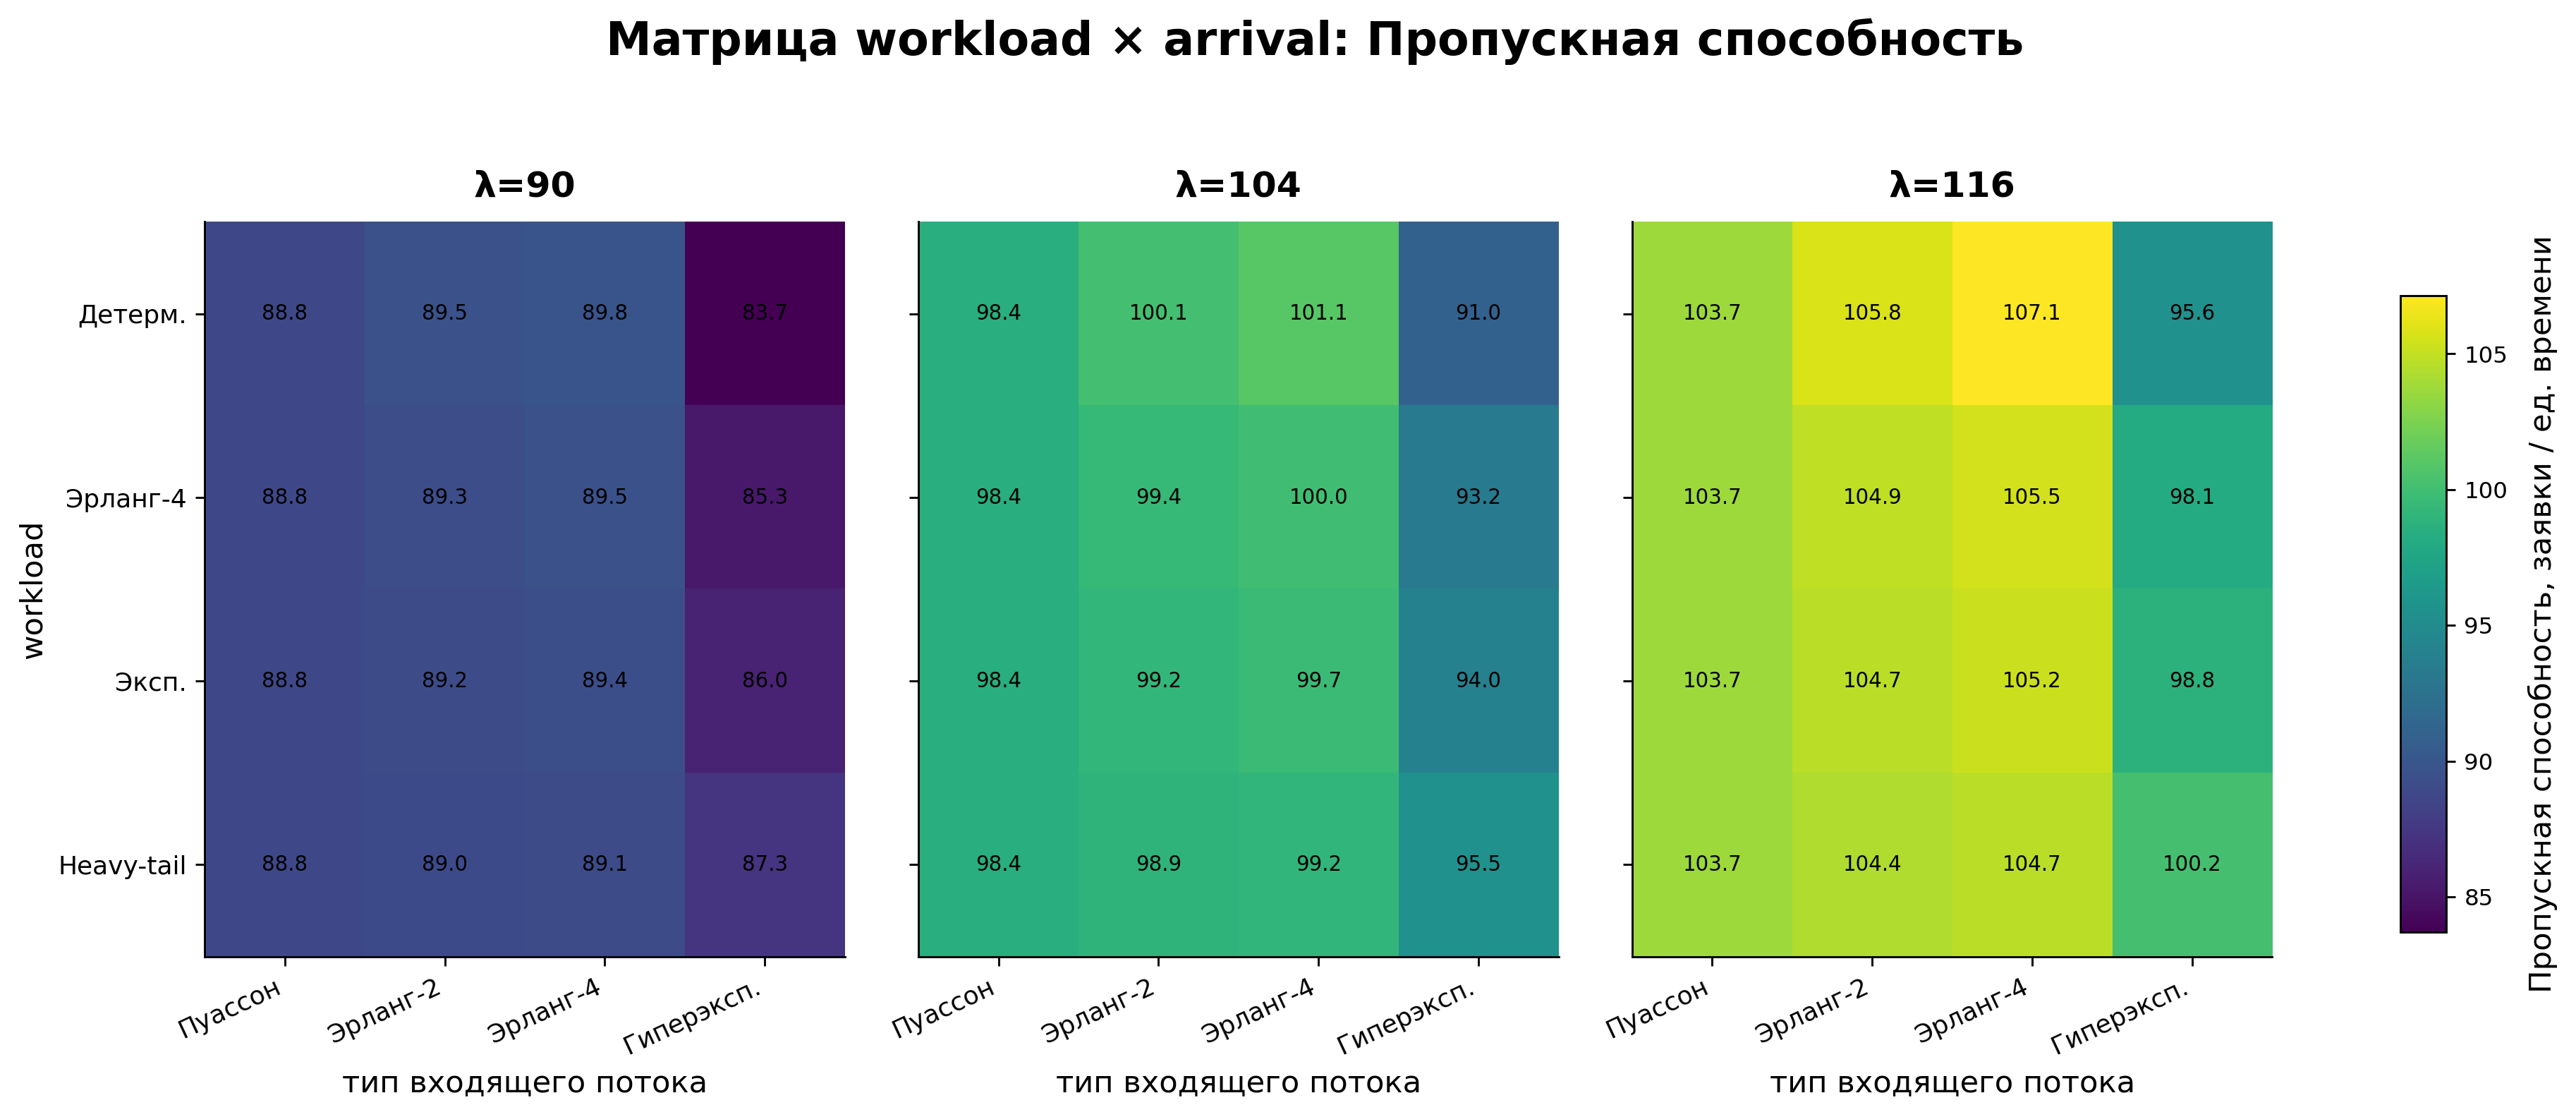
\includegraphics[width=0.95\textwidth]{01_heatmap_workload_arrival_throughput_sigma-1p2}
    \caption{Тепловая карта пропускной способности системы при совместном варьировании распределений}
    \label{fig:comb_heatmap_throughput}
\end{figure}
% 2. Тепловая карта: Средний занятый ресурс
\begin{figure}[H]
    \centering
    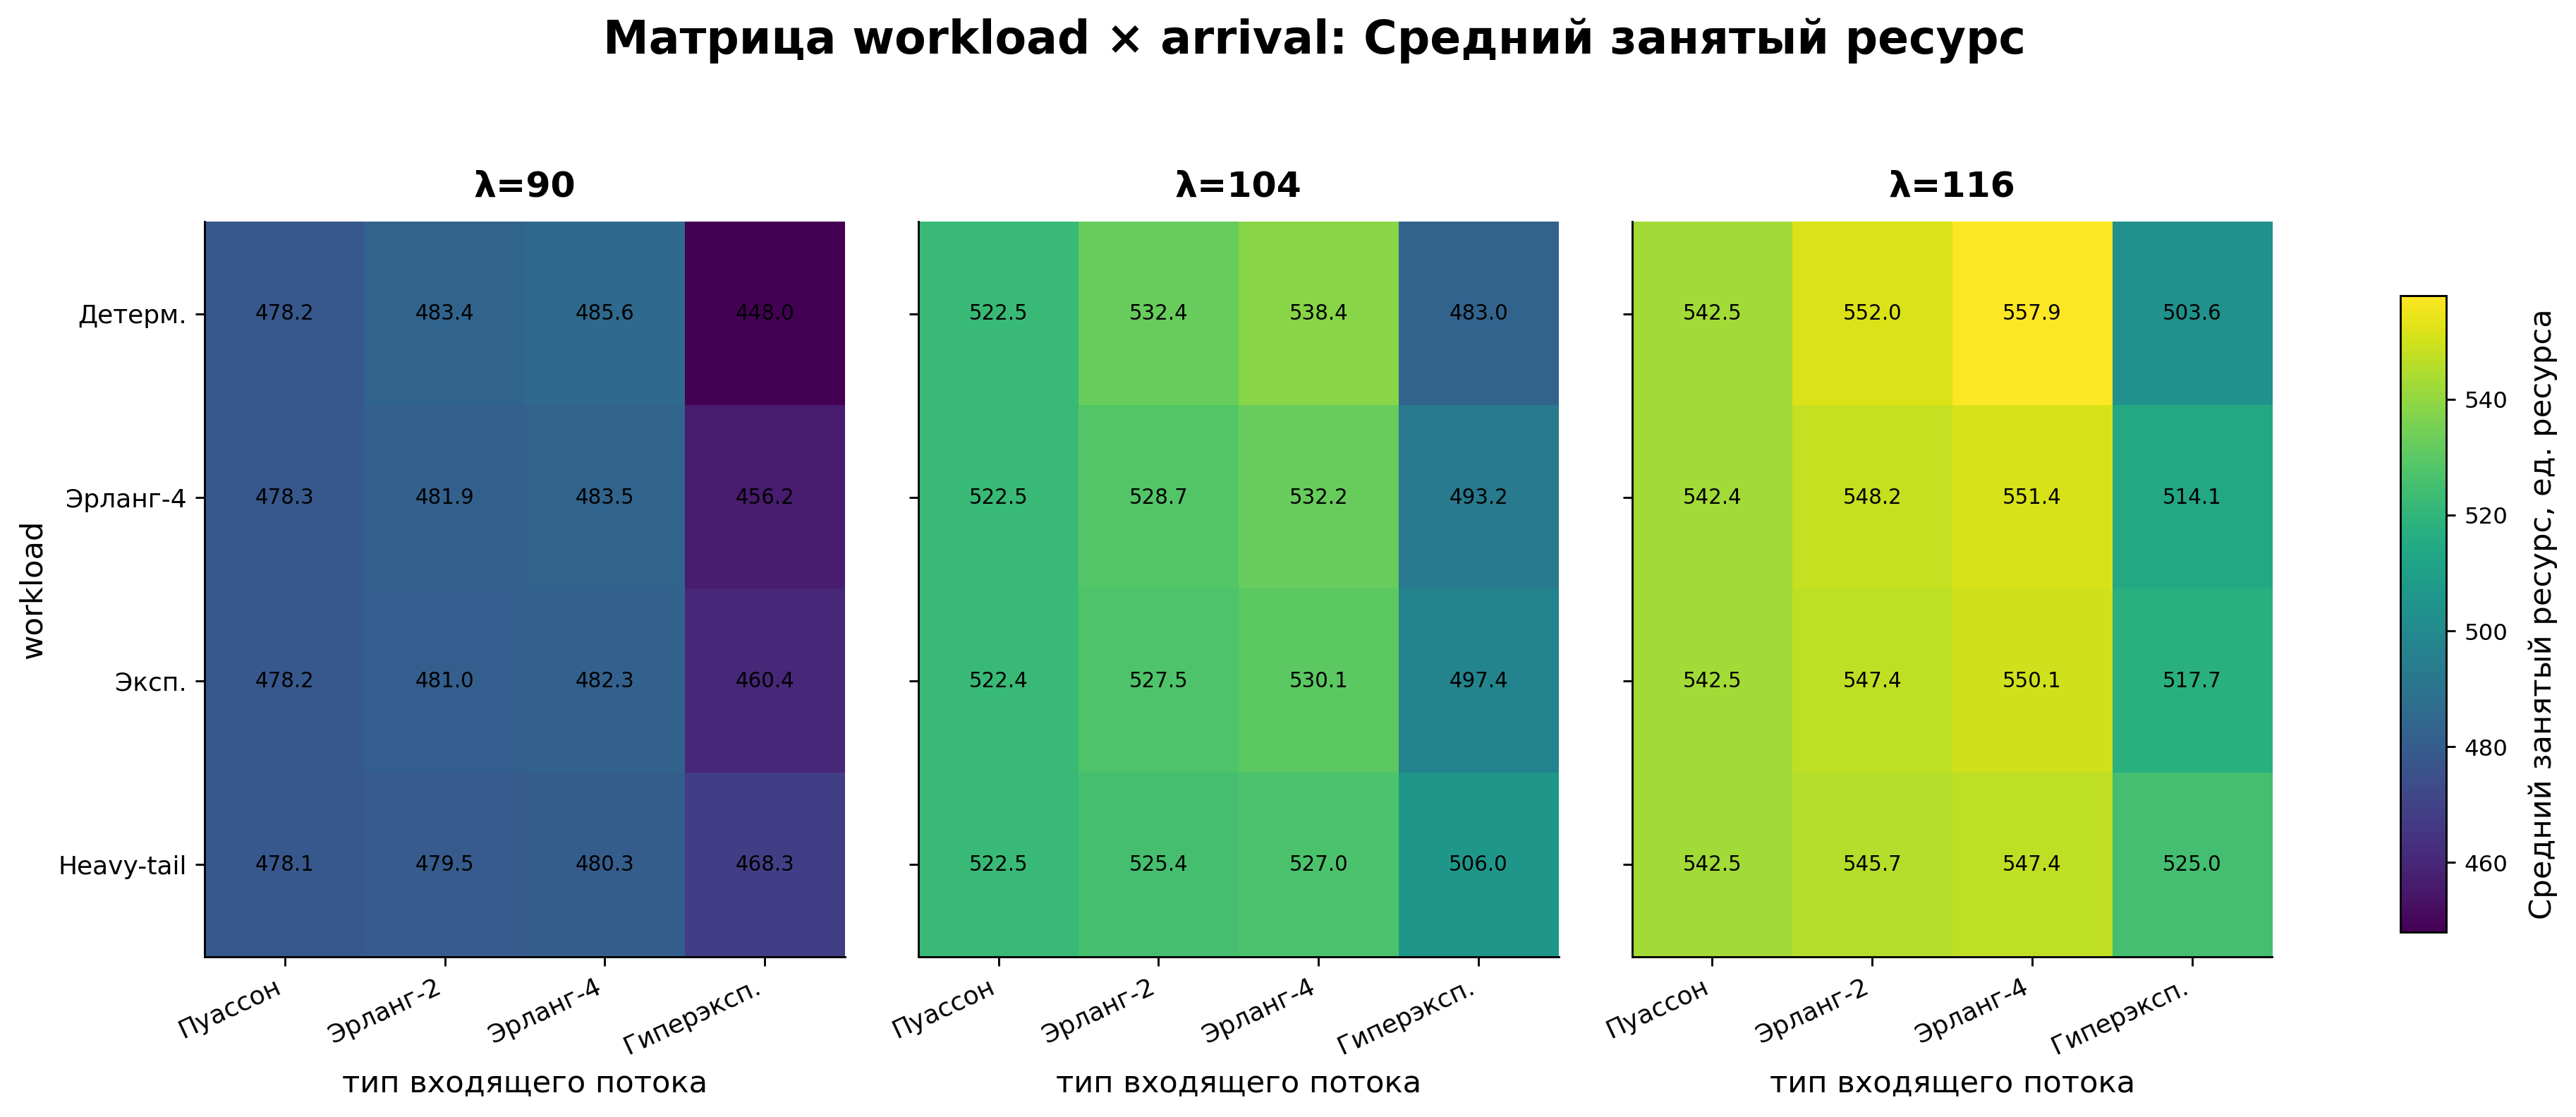
\includegraphics[width=0.95\textwidth]{01_heatmap_workload_arrival_mean_occupied_resource_sigma-1p2}
    \caption{Тепловая карта среднего занятого ресурса при совместном варьировании распределений}
    \label{fig:comb_heatmap_resource}
\end{figure}

Для вероятности отказа совместное смещение относительно базового сценария измеряется в процентных пунктах:
$$
\Delta p_{\mathrm{loss}}(a,\omega,\lambda)
=
100 \cdot
\left(
\widehat{p}_{\mathrm{loss}}(a,\omega,\lambda)
-
\widehat{p}_{\mathrm{loss}}(\text{Poisson},\text{Deterministic},\lambda)
\right).
$$

Для остальных метрик используется относительное отклонение:
$$
\delta_m(a,\omega,\lambda)
=
100 \cdot
\left(
\frac{\widehat{m}(a,\omega,\lambda)}
{\widehat{m}(\text{Poisson},\text{Deterministic},\lambda)}
-
1
\right).
$$

То есть на графиках сравниваются именно отклонения от базового сценария при той же самой интенсивности $\lambda$. Например, на рисунке~\ref{fig:comb_delta_arrival} представлена смещение arrival относительно пуассоновского входа при фиксированном workload.

\begin{figure}[H]
    \centering
    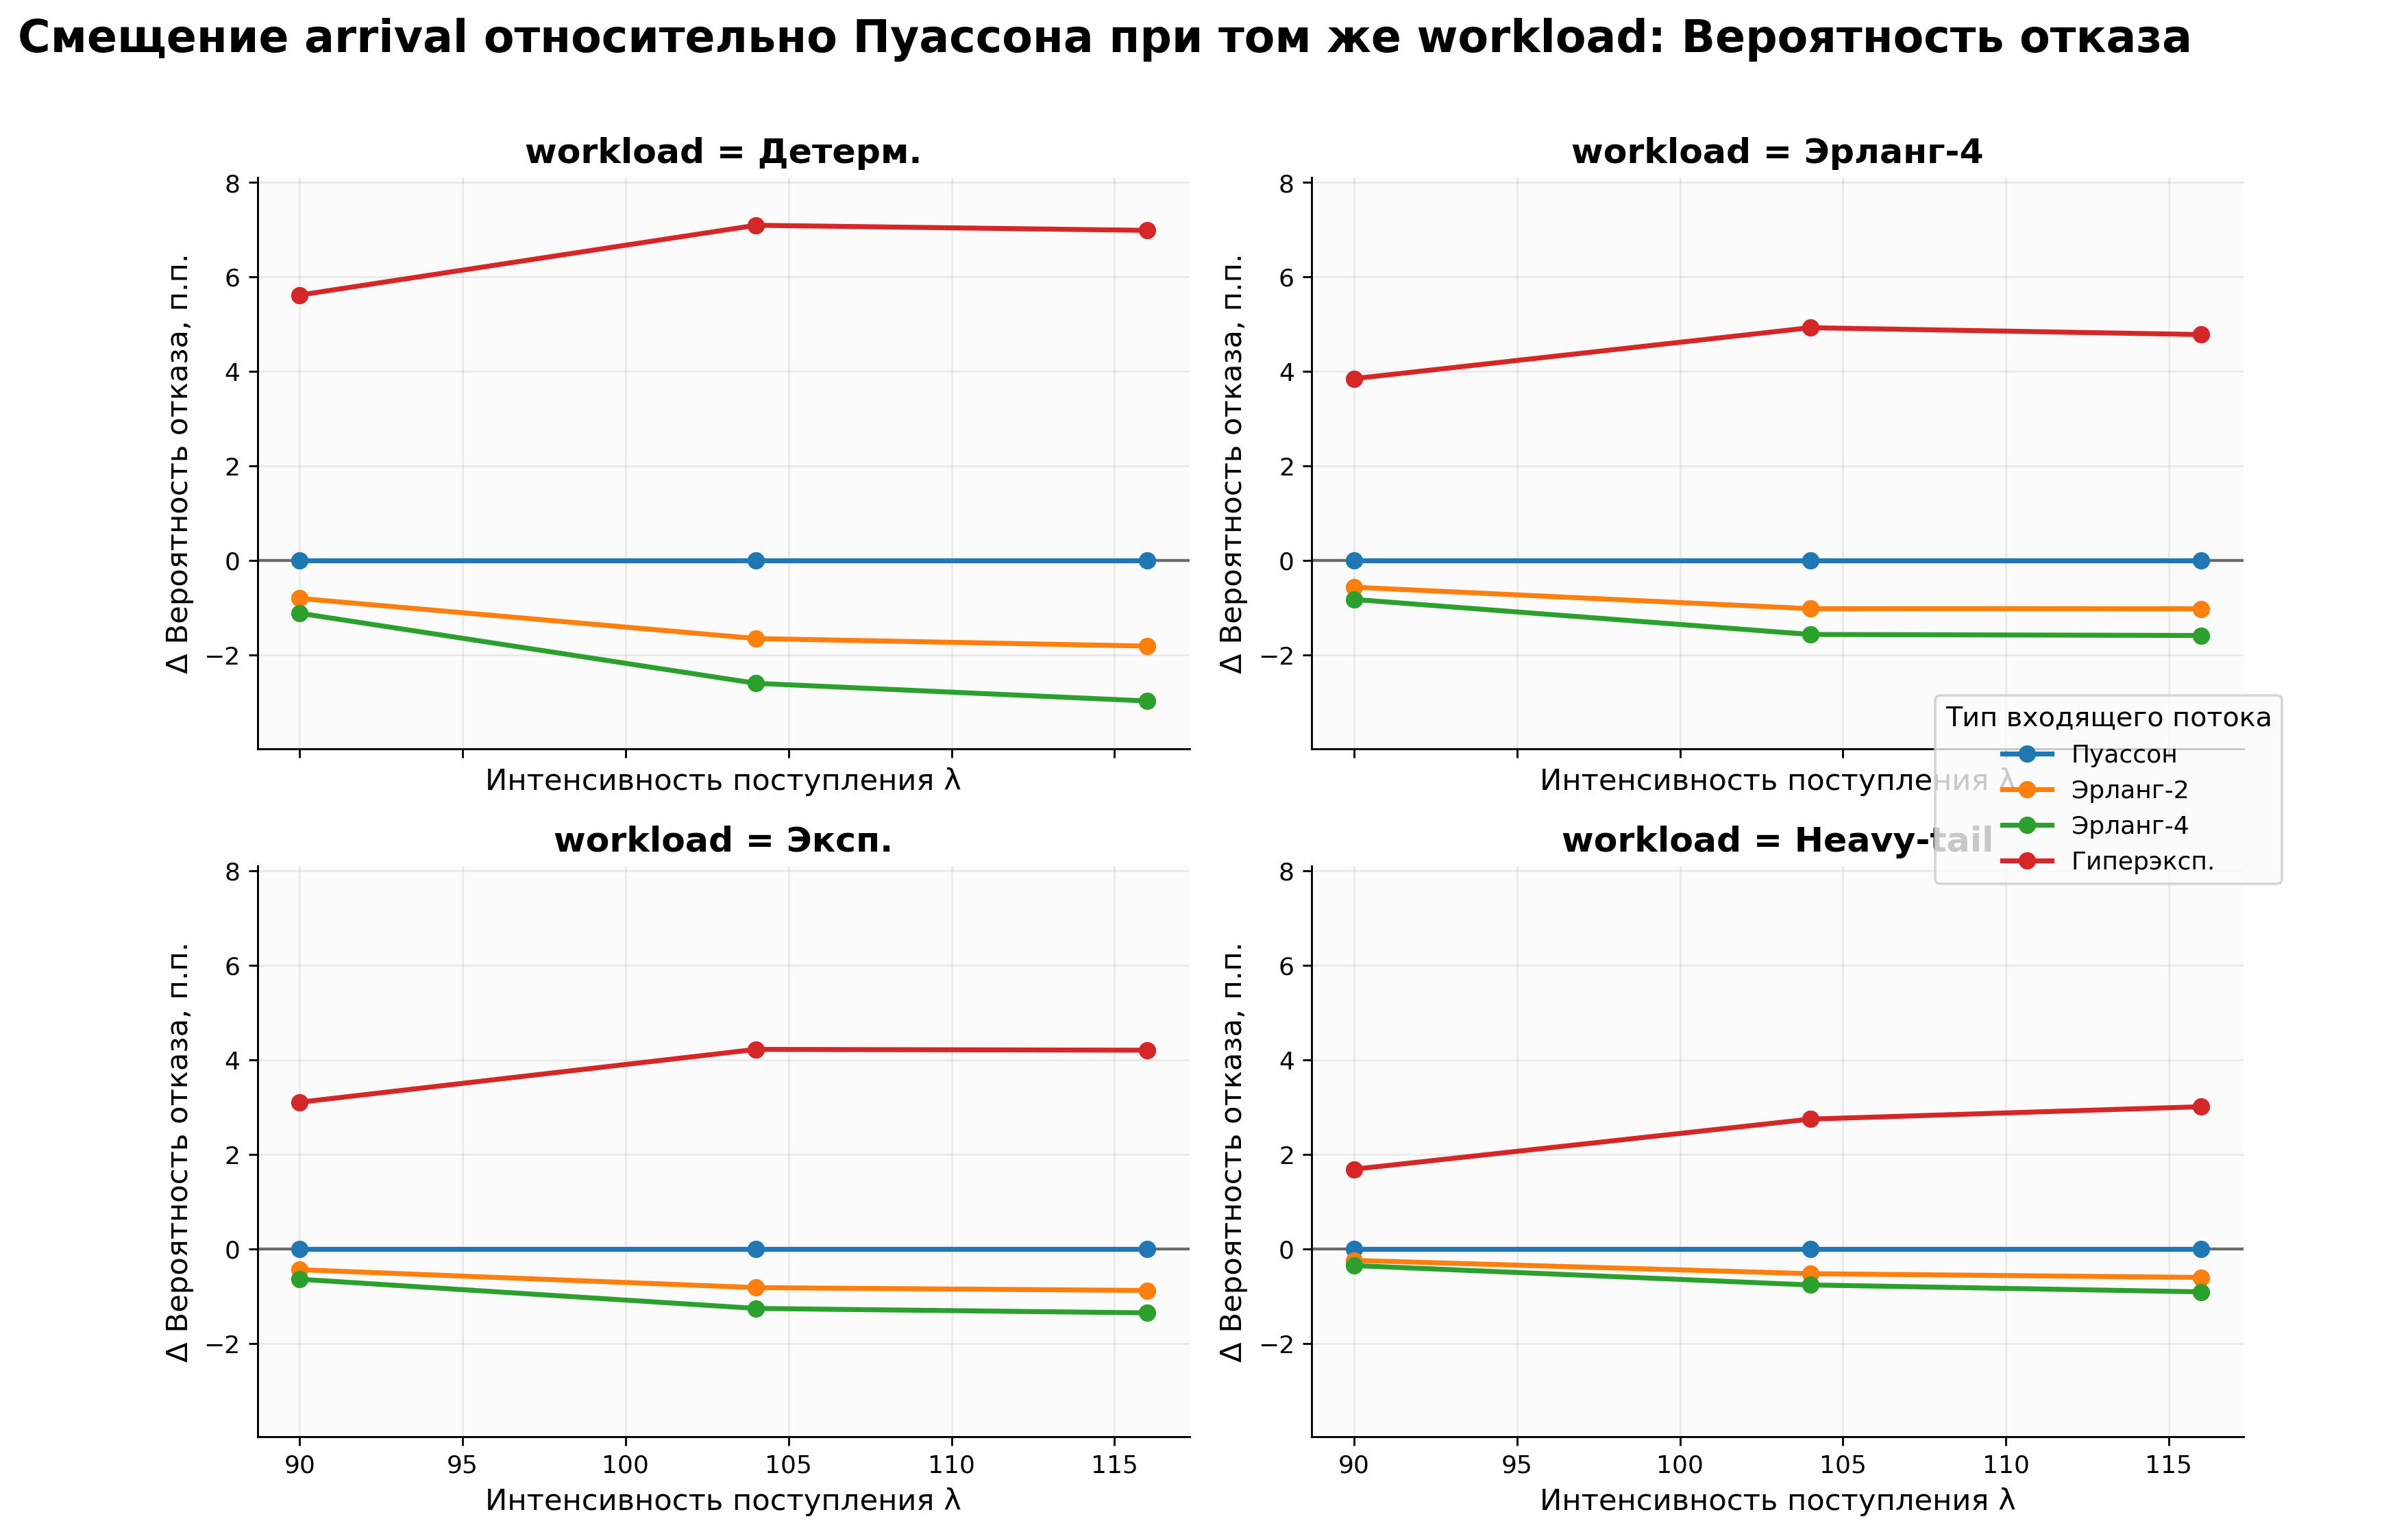
\includegraphics[width=0.95\textwidth]{04_delta_arrival_vs_poisson_by_workload_loss_probability_sigma-1p2}
    \caption{Относительное отклонение вероятности потери от пуассоновского базлайна при различных распределениях обслуживания}
    \label{fig:comb_delta_arrival}
\end{figure}

Для Erlang-потоков $\Delta_A P_{\mathrm{loss}} < 0$, для гиперэкспоненциального входа $\Delta_A P_{\mathrm{loss}} > 0$. При $\lambda=116$ и детерминированном workload, где регуляризация входящего потока снижает вероятность отказа на $1.8\text{-}3.0$ п.п., а bursty-вход увеличивает её почти на $7$ п.п.: $\Delta_A P_{\mathrm{loss}}(\text{Erlang-2,Erlang-4, HyperExp}) = -1.809, -2.970, +6.986$ соответственно.

Распределение workload само по себе не имеет универсального положительного или отрицательного влияния, его эффект определяется типом входящего потока.
% 5. Дельта: Влияние workload при фиксированном arrival (vs Deterministic)
\begin{figure}[H]
    \centering
    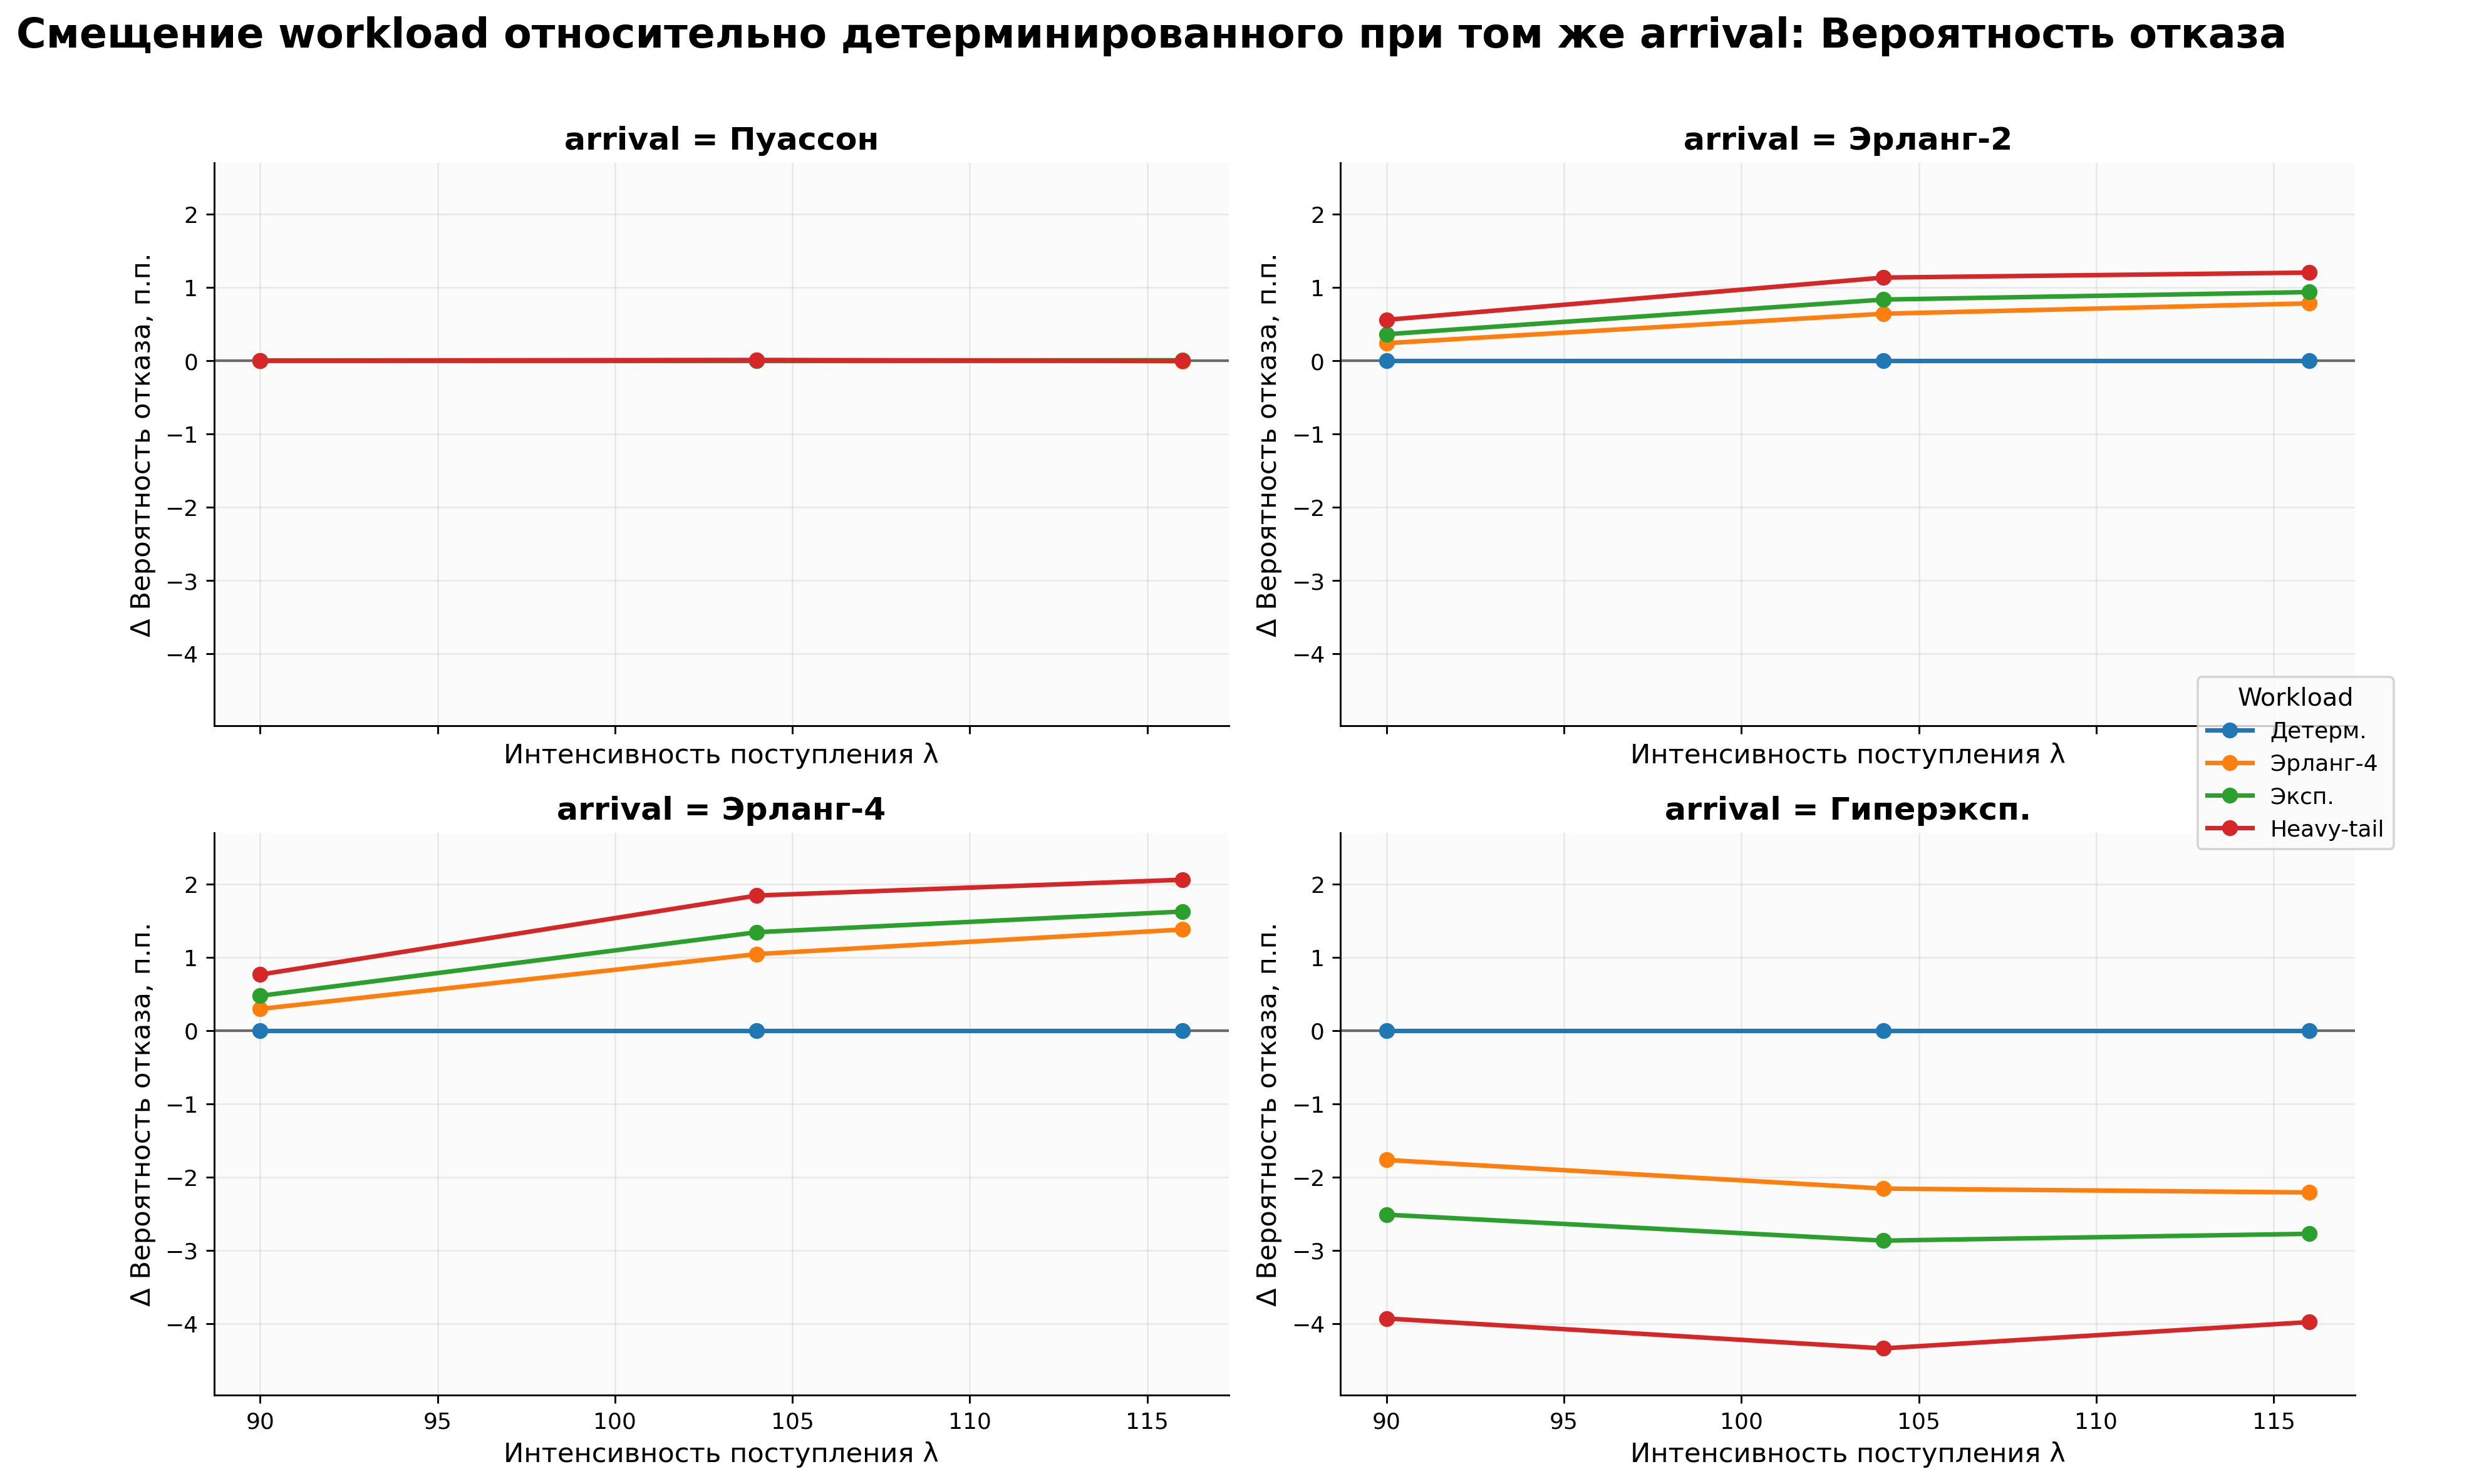
\includegraphics[width=0.95\textwidth]{05_delta_workload_vs_deterministic_by_arrival_loss_probability_sigma-1p2}
    \caption{Относительное отклонение вероятности потери от детерминированного обслуживания при различных входящих потоках}
    \label{fig:comb_delta_workload}
\end{figure}

Структура отказов подтверждает, что главным ограничением в рассматриваемой постановке является ресурс $R$, а затем только число серверов $N$. 
% 7. Структура отказов (Rejection breakdown)
\begin{figure}[H]
    \centering
    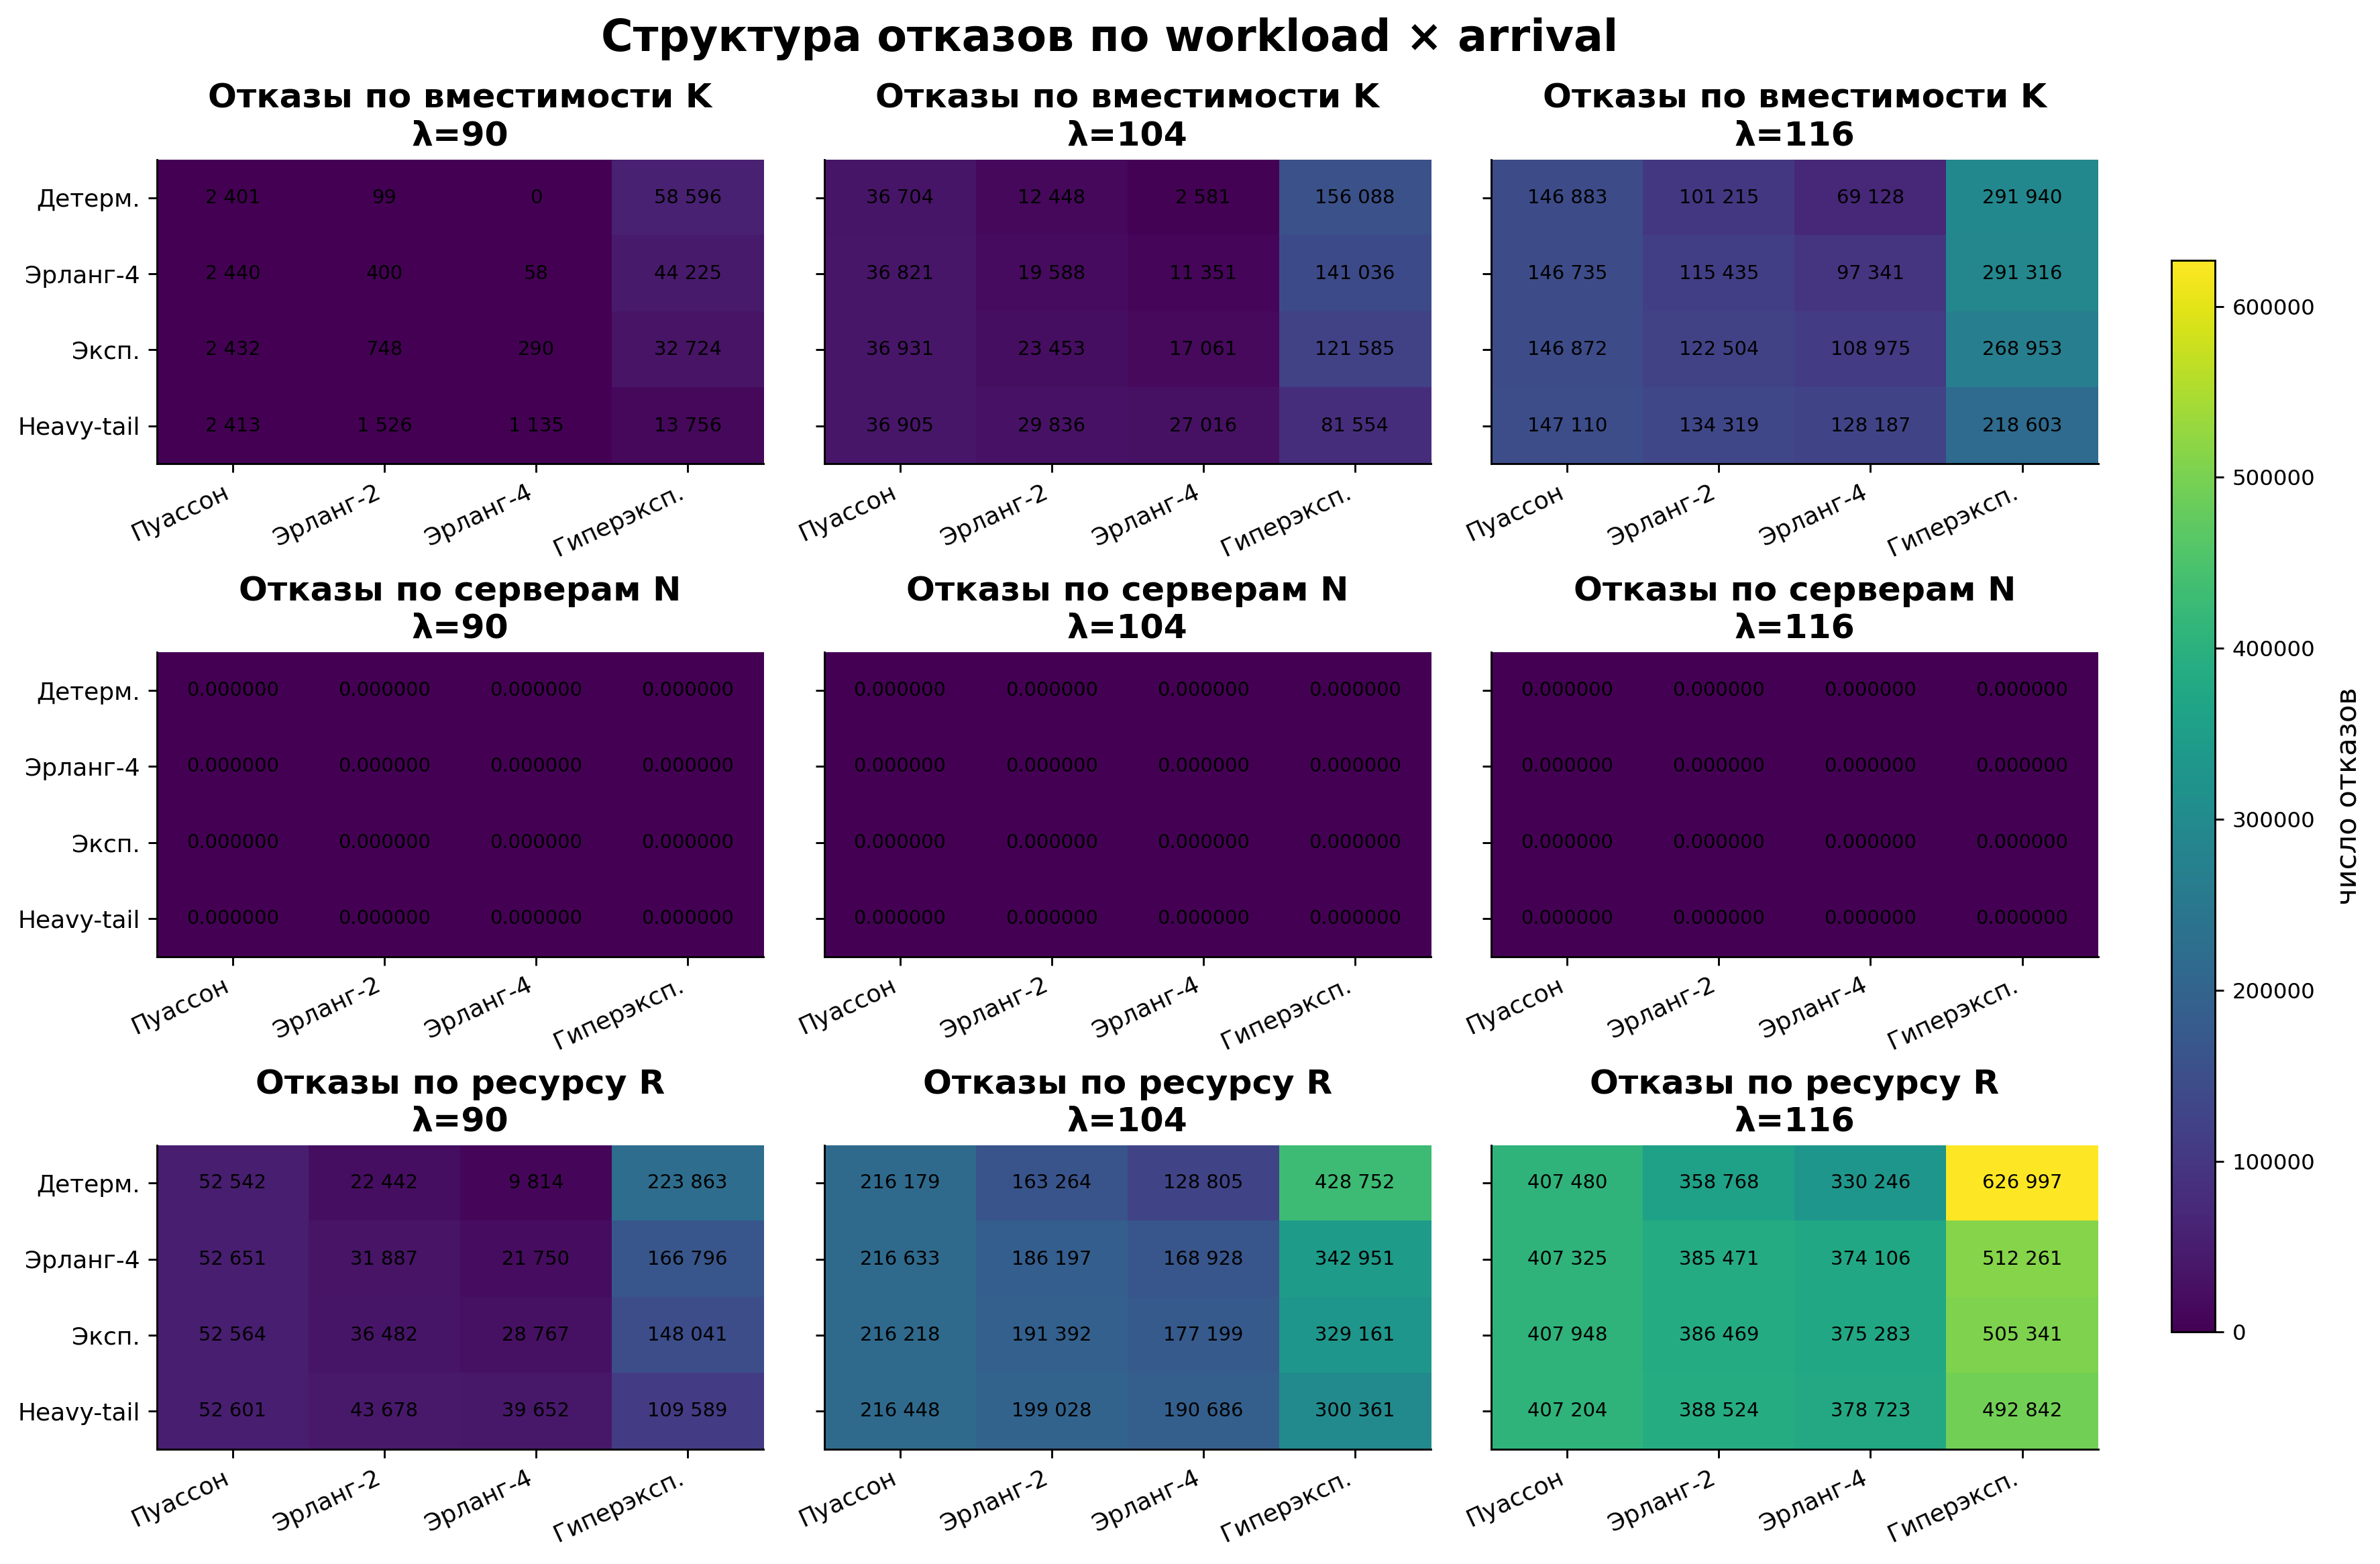
\includegraphics[width=0.95\textwidth]{08_rejection_components_heatmaps_sigma-1p2}
    \caption{Структура отказов (доля блокировок по серверам и по ресурсу) при совместном варьировании распределений}
    \label{fig:comb_rejection_components}
\end{figure}
Менее равномерный вход увеличивает оба типа отказов, но основной вклад даёт именно ограничение по ресурсу. 

\subsection*{Выводы по разделу}

Совместный эксперимент показывает, что чувствительность РСМО с потерями связана с типом входящего потока. При одинаковом $\lambda$ регулярные Erlang-потоки уменьшают вероятность отказа, а гиперэкспоненциальный поток существенно увеличивает её. Сгладить влияние bursty потоков позволяет менее однородное распределение времени работы. 
 Для рассмотренных уровней нагрузки сохраняется порядок:
$$
P_{\mathrm{loss}}(\text{Erlang-4})
<
P_{\mathrm{loss}}(\text{Erlang-2})
<
P_{\mathrm{loss}}(\text{Poisson})
<
P_{\mathrm{loss}}(\text{HyperExp})
$$

Для РСМО с потерями необходимо учитывать прежде всего среднюю нагрузку, затем форму входящего потока и наконец её взаимодействие с распределением времени обслуживания.

% Главная идея:
% Отдельно workload почти слабый фактор.
% Но при непуассоновском входе он взаимодействует с arrival.
% Поэтому полезно ввести interaction effect.

\section{Практическая интерпретация результатов и выводы}
\label{sec:practical_interpretation}

% Главная идея:
% Здесь надо не повторить все графики, а собрать смысл.
%
% Структура:
% 1) что является главным фактором чувствительности;
% 2) где наблюдается инвариантность;
% 3) почему средняя lambda недостаточна;
% 4) что означает структура отказов;
% 5) что ограничивает выводы.

Вычислительные эксперименты проводились для РСМО с потерями $GI/G/N/N/R$ при фиксированных параметрах $N=96$, $R=590$, $\mu=1.2$, $\mathbb{E}[W]=1/\mu=0.833$. Интенсивность входящего потока принимала значения $\lambda \in \{90,104,116\}$. Распределение ресурсного требования $D$ задавалось значениями $2,4,8,12,16$ с вероятностями $0.25,0.25,0.30,0.15,0.05$, поэтому $\mathbb{E}[D]=6.5$. Каждый сценарий оценивался по $40$ независимым репликациям.

Основным фактором чувствительности в рассматриваемой системе является тип входящего потока. Различные распределения $A$ приводят к разнообразным значениям вероятности отказа, пропускной способности и средней занятости ресурса. Регулярные потоки Эрланга уменьшают вероятность отказа, а гиперэкспоненциальный поток, моделирующий всплески поступлений, существенно её увеличивает.

Вторым по значению фактором чувствительности является средняя интенсивность потока $\lambda$. 

Распределение объёма работы заявки $W$ при пуассоновском входящем потоке подтверждает свойство инвариантности системы. При непуассоновском входе инвариантность нарушается. Распределение времени обслуживания зависит от входящего потока заявок и может улучшить отказоустойчивость: при равномерном входящем потоке выигрыш дает равномерное распределение workload, при крайне неравномерном входящем потоке burstly workload позволяет снизить потери. Лучшим сочетанием является Erlang-4 входящий поток и deterministic workload, худшим гиперэкспоненциальный входящий поток и deterministic workload.

Декомпозиция отказов показывает, что в выбранной конфигурации главным ограничивающим фактором является ресурс $R$.

\clearpage

%  Заключение
\chapter*{ЗАКЛЮЧЕНИЕ}
\addcontentsline{toc}{chapter}{ЗАКЛЮЧЕНИЕ}
В работе была исследована РСМО с потерями вида $GI/G/N/N/K$, в которой каждая поступающая заявки занимает 1 прибор и случайный объем ограниченного ресурса. Основное внимание было уделено анализу чувствительности стационарных характеристик системы к форме распределения входящего потока и распределения объема работы заявки при фиксированных первых моментах.

Начиная с классической модели Эрланга $M/M/N/N$ рассматривались все более общие случаи. Сначала при генерализации распределения времени работы в $M/G/N/N$ системе проявляется свойство инвариантности к режиму работы заявки. Затем рассмотрелись ресурсные системы $M/G/N/N/R$, которые добавили дополнительное условие к причинам отказа заявки. И наконец с учетом современных исследований трафика было генерализировано распределение входящего потока заявок. Наличие случайного ресурсного требования и отказ от пуассоновского входящего потока приводят к потере марковского свойства и резкому росту пространства состояний.

Во второй главе была формализована математическая модель РСМО с потерями, учитывающая ограничения по прибору ($N$) и ресурсу ($R$). Состояние системы в произвольный момент времени описано через текущее число заявок $\xi(t)$ и суммарный объем занятого ими ресурса $\delta(t)$. Поступающая заявка с требованием $r_i$ теряется при выполнении хотя бы одного из условий: $\xi(t-) = N$ или $\delta(t-) + r_i > R$. В качестве целевых метрик эффективности исследованы вероятность отказа ($P_{\mathrm{loss}}$), абсолютная пропускная способность ($\theta$), математическое ожидание занятого ресурса $\mathbb{E}[\delta]$ и оценка стационарного распределения вероятностей состояний $\pi(k)$. 

Для оценки стационарных характеристик системы был разработан алгоритм и дискретно-событийного имитационного моделирования методом Монте-Карло. Чтобы отделить влияние средней нагрузки от влияния формы распределений, в вычислительном эксперименте задавались семейства распределений входящего потока и объема работы заявки с идентичными математическими ожиданиями, но различными коэффициентами вариации $c_v$. 

Для распределения интервалов между заявками были выбраны базовое пуассоновское распределение ($c_v = 1$), распределения Эрланга 4-го и 2-го порядков ($c_v = 0.5$ и $c_v \approx 0.71$) соответственно, моделирующие регулярные потоки и гиперэкспоненциальное распределение ($c_v > 1$, моделирующее пачечный характер трафика и тяжелые хвосты).

Для распределения времени работы заявки было взять базовое детерменированное распределение ($c_v = 0$), экспоненциальное ($c_v = 1$), распределение Эрланга 4го порядка ($c_v = 0.5$) и гиперэкспоненциальное ($c_v > 1$). 

Особое внимание в работе уделено архитектуре программного комплекса. Учитывая отсутствие буфера ожидания и, как следствие, отсутствие необходимости динамически выделять память под отслеживание объектов в очереди, каждая репликация Монте-Карло представляет собой независимый процесс. Все $960$ потоков, полученные благодаря трем значениям $\lambda$, четырем распределениям интенсивности входящего потока, четырем распределениям времени работы заявки при 40 репликацияз  запускаются параллельно на ядрах CUDA. Это обеспечивает прирост производительности по сравнению с CPU. 

Подтвердилось свойство инвариантности ресурсной системы с потерями к распределению времени обслуживания при пуассоновском входящем потоке. При сохранении одинакового среднего времени обслуживания переход от детерминированного распределения к экспоненциальному, эрланговскому или гиперэкспоненциальному распределению практически не изменял вероятность отказа, пропускную способность и среднюю занятость системы. Наблюдаемые расхождения находились на уровне статистического шума метода Монте-Карло.

Тип входящего потока оказался более существенным фактором чувствительности РСМО. При одинаковой средней интенсивности $\lambda$ регулярные потоки Эрланга приводили к снижению вероятности отказа и более устойчивому заполнению системы, тогда как гиперэкспоненциальный входящий поток, моделирующий всплески поступлений, существенно увеличивал вероятность отказа. 

Различная интенсивность входящего потока $\lambda$, моделирующая низкую, среднюю и высокую нагрузку, оказалась самым существенным фактором влияния на вероятность отказа, пропускную способность и среднюю занятость системы. 

Совместный анализ распределений входящего потока и времени обслуживания показал, что при непуассоновском входе свойство инвариантности нарушается. Для регулярных входящих потоков наилучшие результаты дает более регулярное обслуживание, тогда как при всплесковом гиперэкспоненциальном входе повышение вариативности времени обслуживания может частично снижать вероятность отказа за счет более неравномерного освобождения ресурсов. Таким образом, распределение времени обслуживания само по себе не имеет универсального положительного или отрицательного эффекта: его влияние проявляется через взаимодействие с характером входящего потока.

Таким образом в ходе работы была построена и исследована имитационная модель ресурсной системы с потерями $GI/G/N/N/R$, разработан программно-вычислительный комплекс для проведения серии экспериментов, а также выявлены основные факторы чувствительности стационарных характеристик. Полученные результаты показывают, что для ресурсных СМО с потерями в первую очередь необходимо учитывать среднюю нагрузку и тип входящего потока, затем --- взаимодействие входящего потока с распределением времени обслуживания. 




\clearpage

%  Список использованных источников
\phantomsection
\printbibliography[heading=bibintoc, title={СПИСОК ИСПОЛЬЗОВАННЫХ ИСТОЧНИКОВ}]
\clearpage

%  Приложения
\appendix

\chapter{Дополнительные материалы вычислительного эксперимента}
\label{app:additional_materials}

\section{Параметры эксперимента и структура данных}
\label{app:params}

\begin{table}[H]
\centering
\caption{Структура выходных файлов вычислительного комплекса}
\label{tab:output_files}
\begin{tabularx}{\textwidth}{|l|X|}
\hline
\textbf{Файл / Директория} & \textbf{Содержание} \\ \hline
\texttt{suite\_result.json} & Полный результат серии: конфигурация сценариев, число репликаций, точечные оценки метрик, доверительные интервалы, стационарные распределения \\ \hline
\texttt{aggregated\_summary.csv} & Сводная таблица по всем сценариям в удобном табличном виде \\ \hline
\texttt{metric\_summaries.csv} & Таблица статистических характеристик по отдельным целевым метрикам \\ \hline
\texttt{run\_summaries.csv} & Детализированные результаты независимых репликаций (Монте-Карло) \\ \hline
\texttt{suite\_summary.txt} & Текстовая сводка параметров запущенной серии \\ \hline
\texttt{plots/} & Автоматически сгенерированные графики для базовых экспериментов \\ \hline
\texttt{plots\_reworked3/} & Графики совместного анализа чувствительности (тепловые карты, срезы) \\ \hline
\end{tabularx}
\end{table}

\textbf{Пример конфигурационного файла (фрагмент \texttt{suite\_result.json}):}
\begin{verbatim}
{
  "suite_name": "baseline_gpu",
  "replications": 40,
  "max_time": 50000.0,
  "warmup_time": 5000.0,
  "servers_n": 96,
  "total_resource_r": 590,
  "arrival_rate_levels": [90.0, 104.0, 116.0],
  "service_speed_levels": [1.2],
  "resource_values": 
  [2, 4, 8, 12, 16],
  "resource_probabilities": 
  [0.25, 0.25, 0.3, 0.15, 0.05],
  "workload_family_basic": 
  [
    "deterministic", 
    "exponential", 
    "erlang_4", 
    "hyperexp_heavy"
    ],
  "arrival_process_family": 
  [
    "poisson", 
    "erlang_2", 
    "erlang_4", 
    "hyperexp_2"
    ]
}
\end{verbatim}

\clearpage
\section{Дополнительные графики чувствительности к workload}
\label{app:workload_plots}

На рисунке~\ref{fig:app_workload_boxplots} показано, что дисперсия результатов Монте-Карло для различных метрик на уровне нагрузки $\lambda=90$ сопоставима с изменениями от типа распределения времени обслуживания, что подтверждает вывод об инвариантности.

\begin{figure}[H]
    \centering
    \begin{subfigure}{0.48\textwidth}
        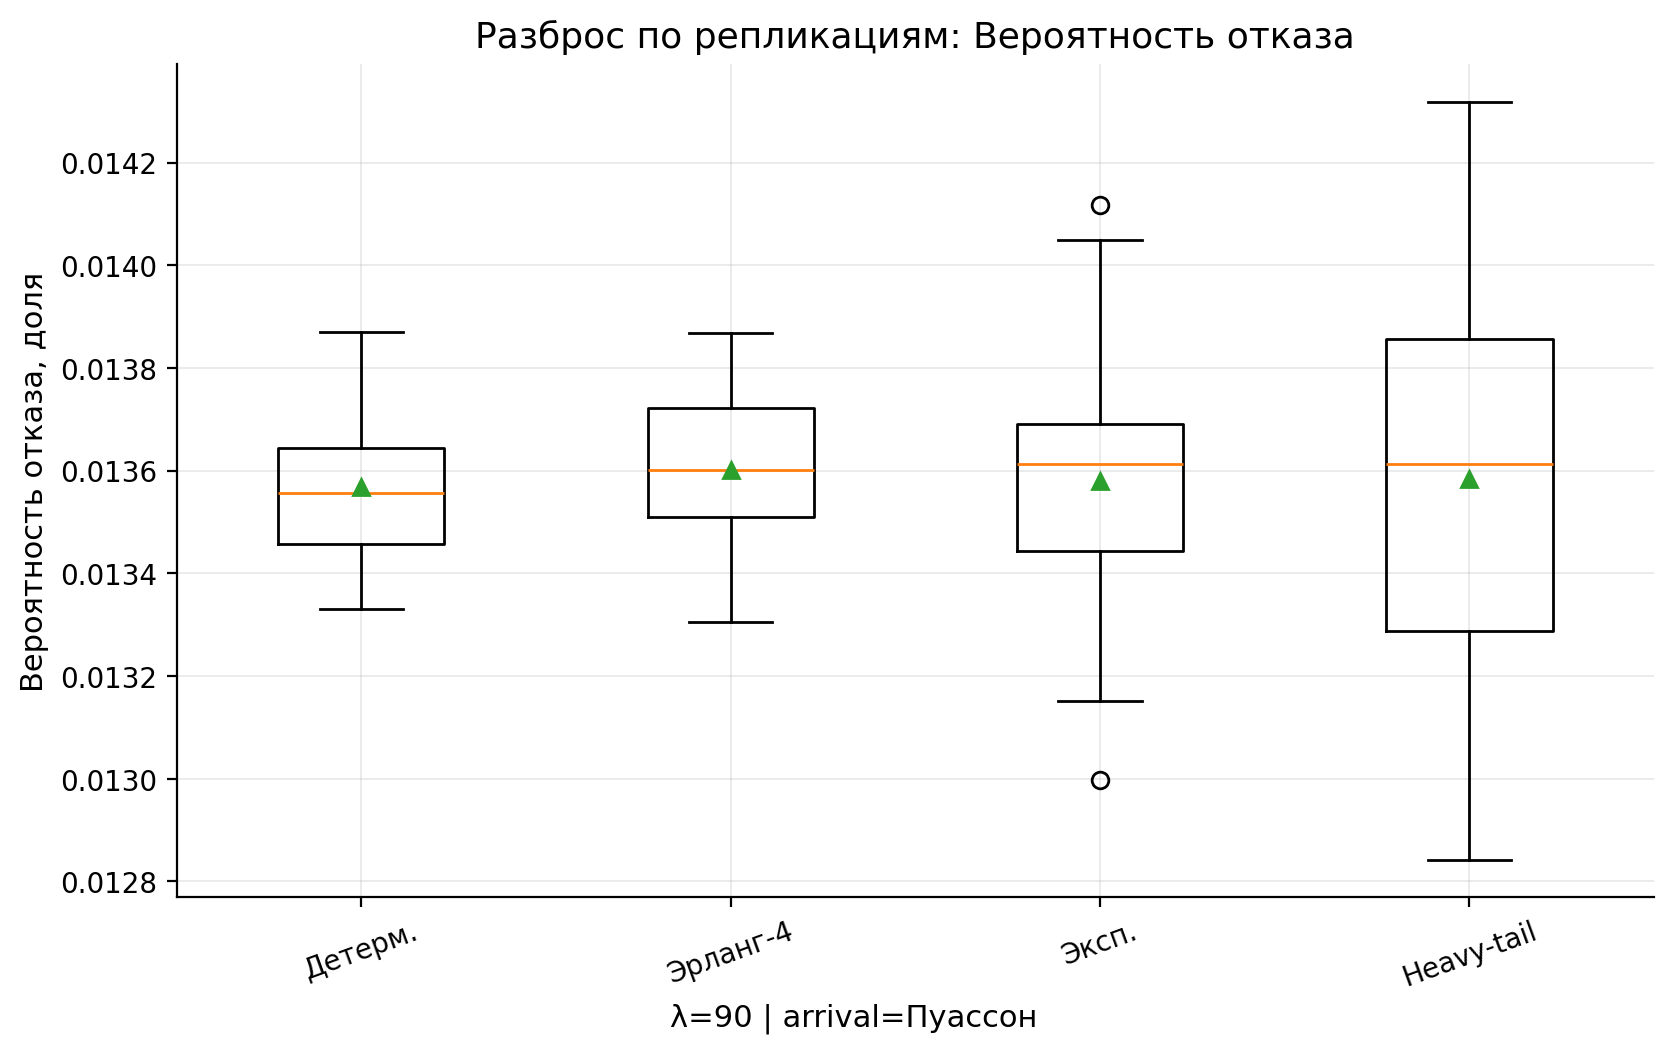
\includegraphics[width=\textwidth]{workload_sensitivity_boxplot_loss_probability_sigma-1p2_lambda-90.png}
        \caption{Вероятность потери}
    \end{subfigure}
    \hfill
    \begin{subfigure}{0.48\textwidth}
        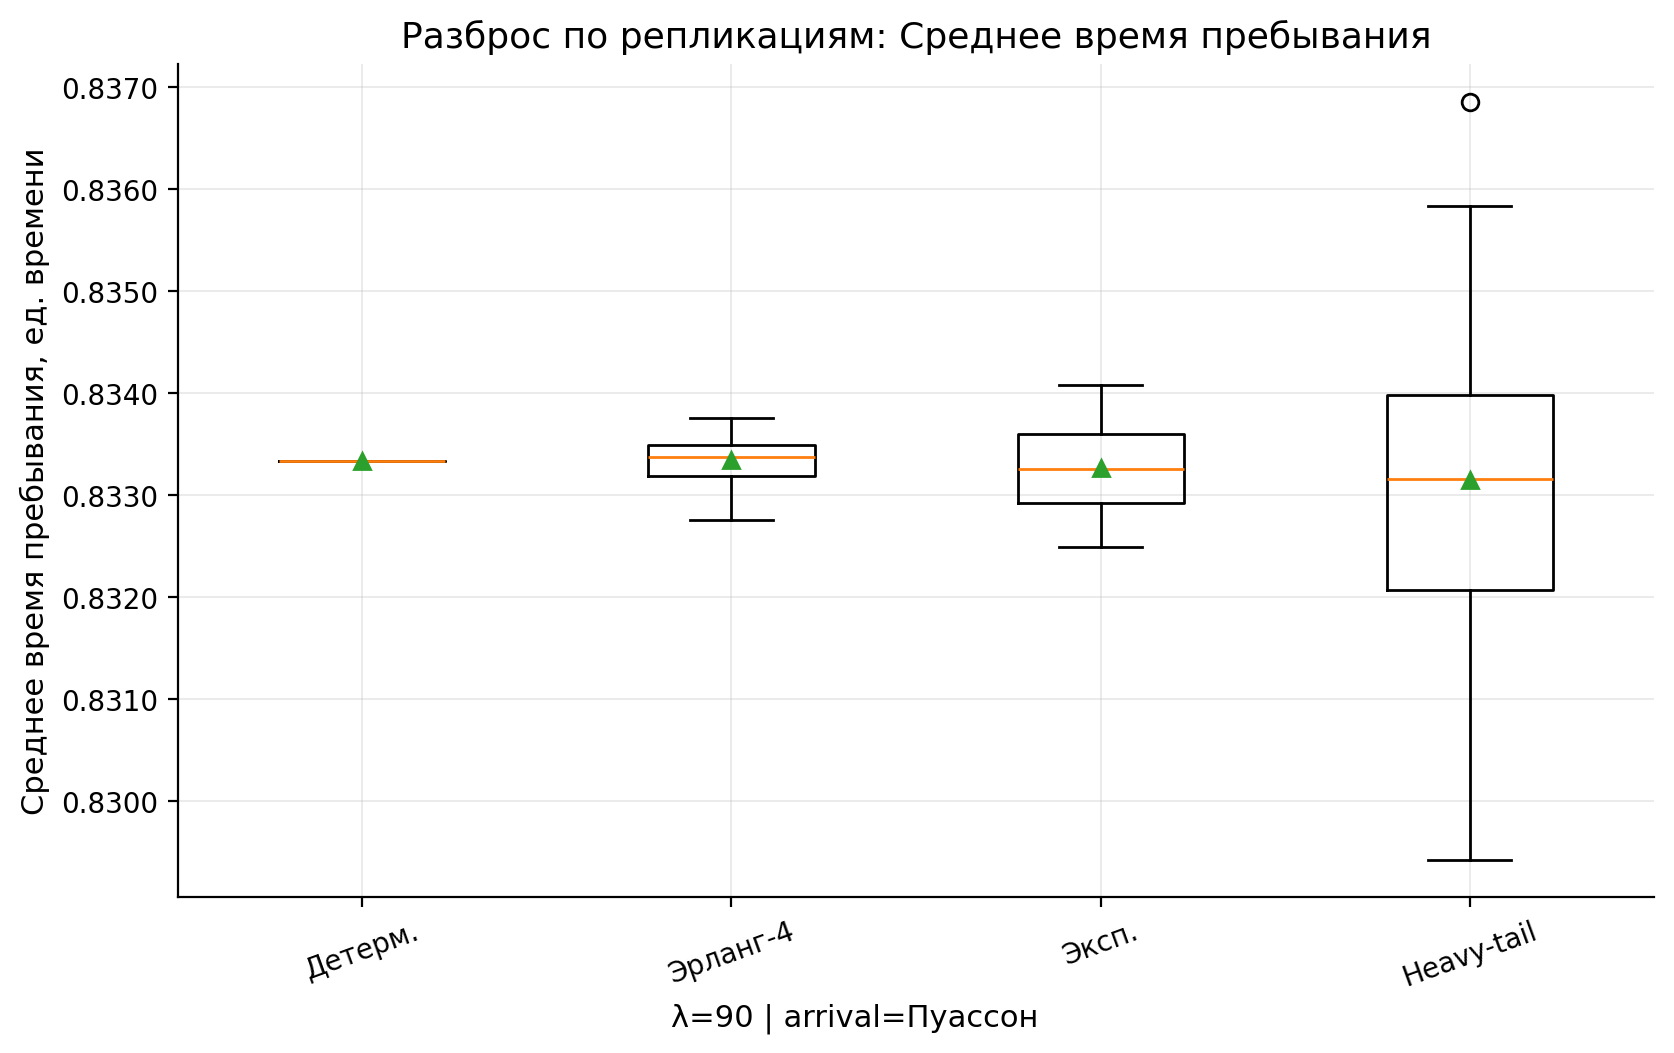
\includegraphics[width=\textwidth]{workload_sensitivity_boxplot_mean_sojourn_time_sigma-1p2_lambda-90.png}
        \caption{Среднее время пребывания}
    \end{subfigure}
    \caption{Разброс целевых метрик по репликациям в зависимости от workload ($\lambda = 90$)}
    \label{fig:app_workload_boxplots}
\end{figure}

\begin{figure}[H]
    \centering
    \begin{subfigure}{0.48\textwidth}
        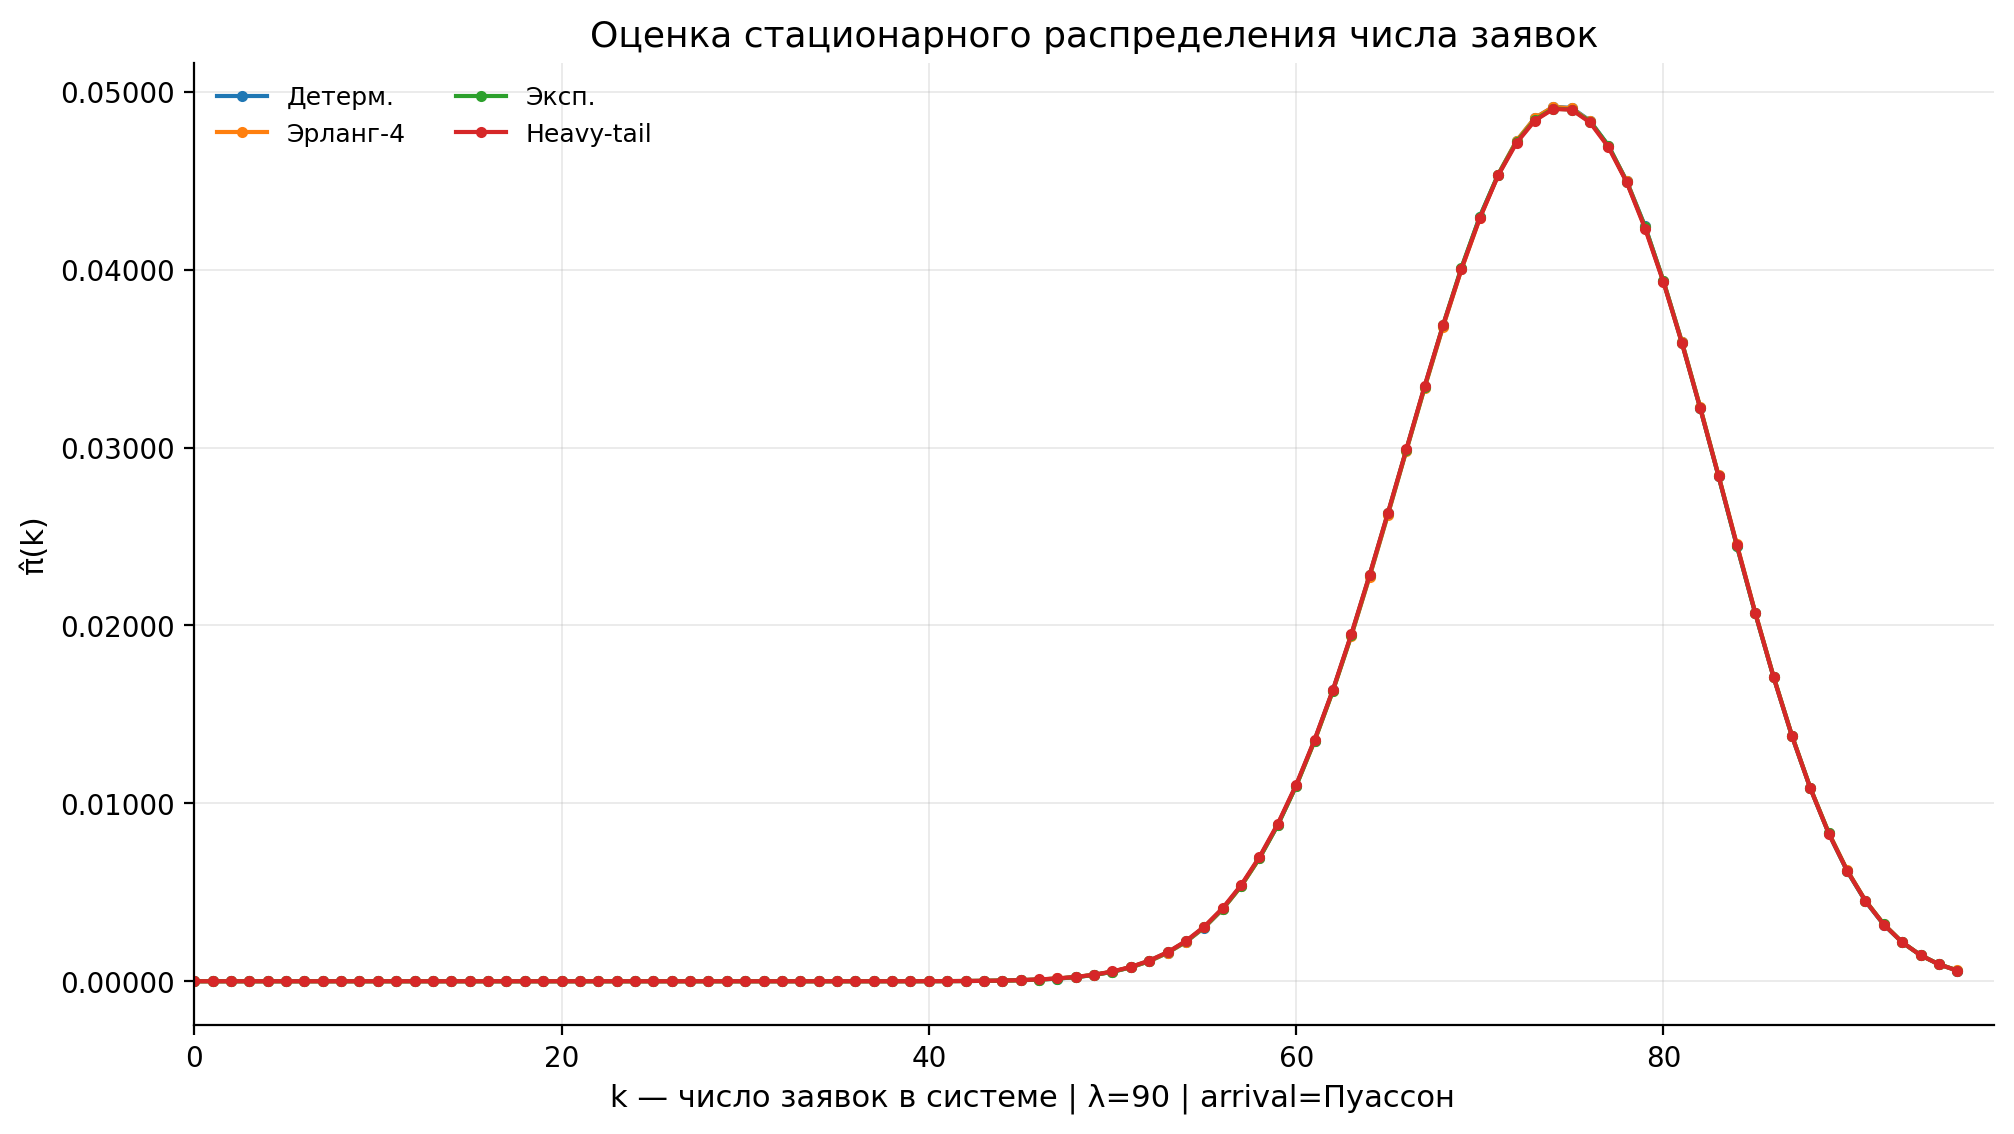
\includegraphics[width=\textwidth]{workload_sensitivity_stationary_distribution_sigma-1p2_lambda-90.png}
        \caption{Общий вид $\pi(k)$}
    \end{subfigure}
    \hfill
    \begin{subfigure}{0.48\textwidth}
        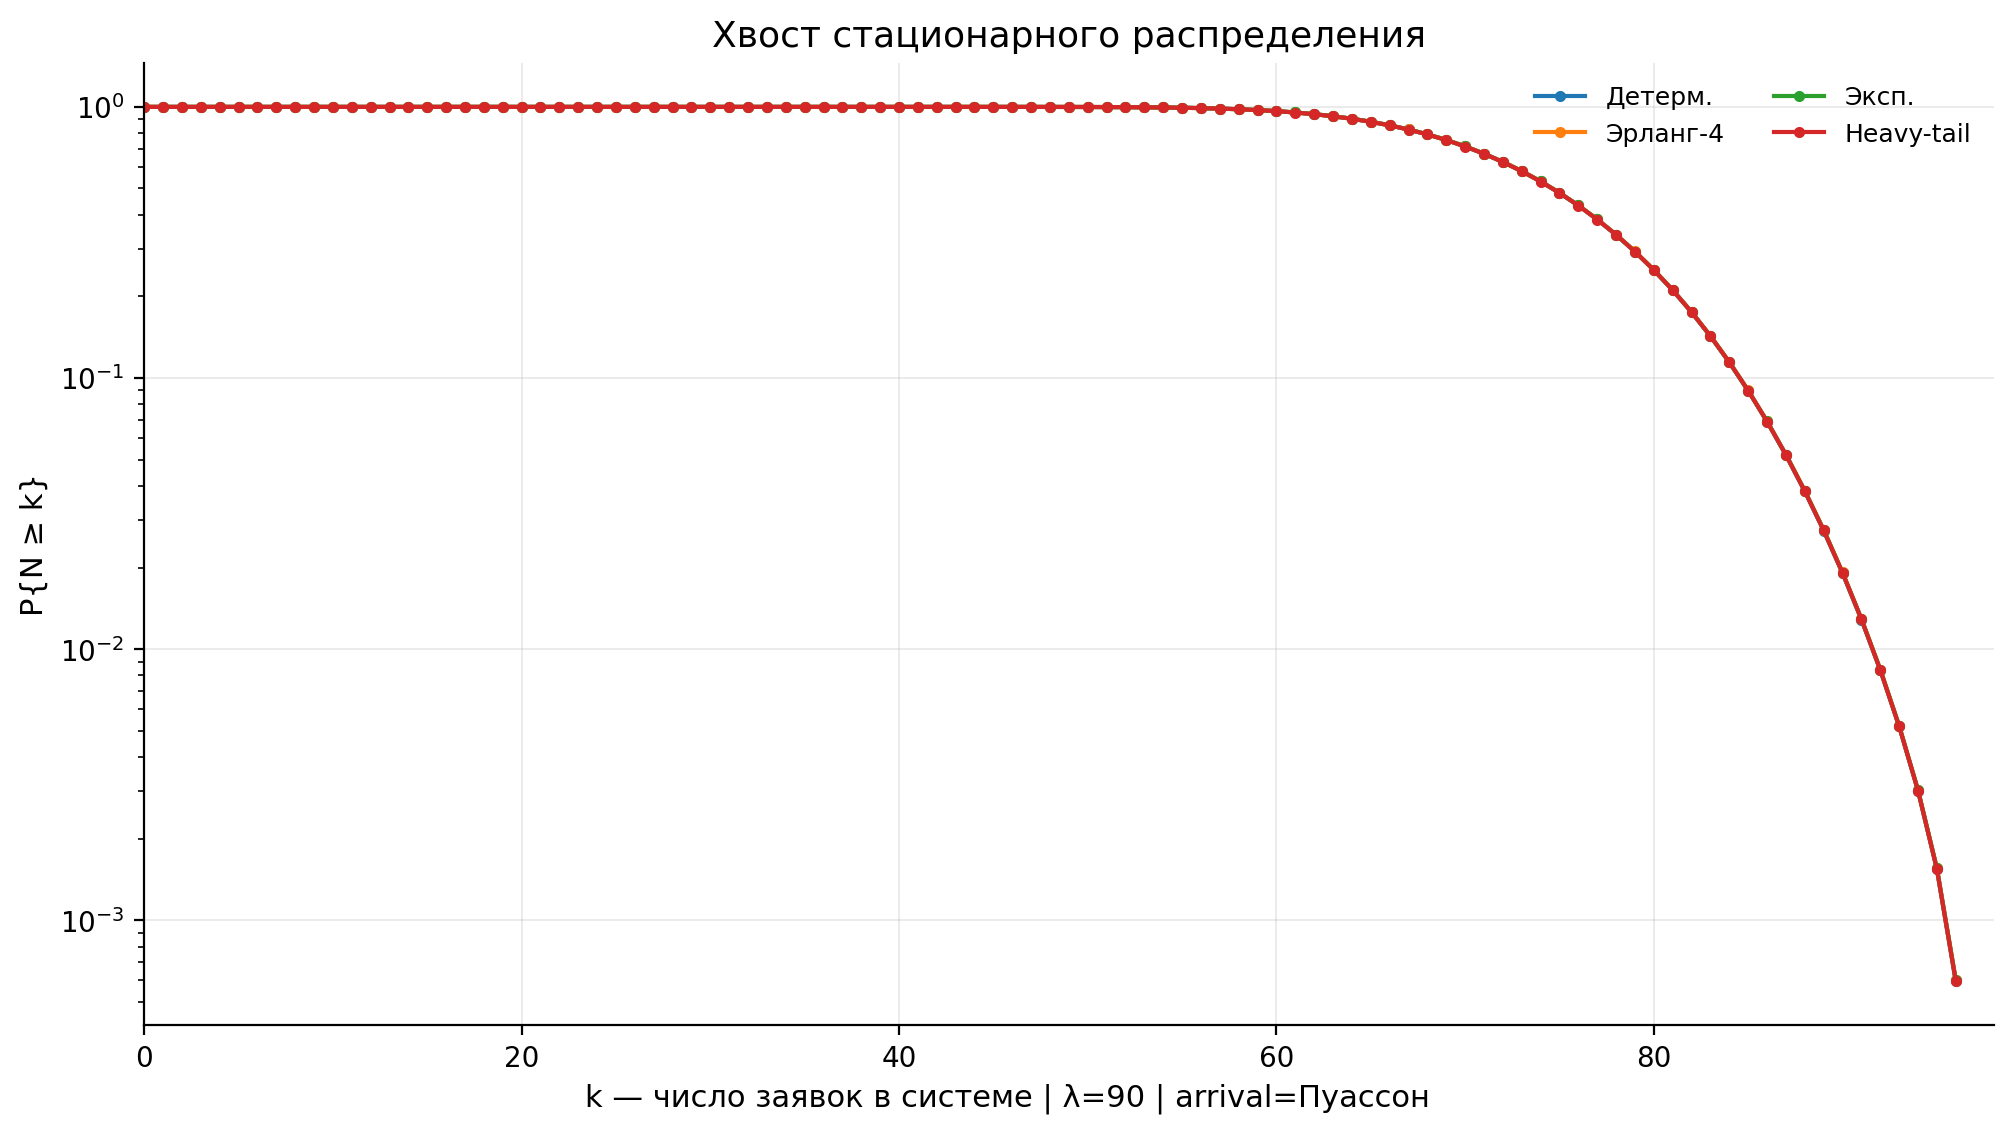
\includegraphics[width=\textwidth]{workload_sensitivity_stationary_tail_sigma-1p2_lambda-90.png}
        \caption{Хвостовые вероятности}
    \end{subfigure}
    \caption{Стационарное распределение числа заявок в системе при изменении workload ($\lambda = 90$)}
    \label{fig:app_workload_stationary}
\end{figure}


\clearpage
\section{Дополнительные графики чувствительности к входящему потоку}
\label{app:arrival_plots}

На рисунке~\ref{fig:app_arrival_boxplots} проиллюстрировано статистически значимое влияние типа входящего потока на метрики при невысокой нагрузке ($\lambda=90$). 

\begin{figure}[H]
    \centering
    \begin{subfigure}{0.48\textwidth}
        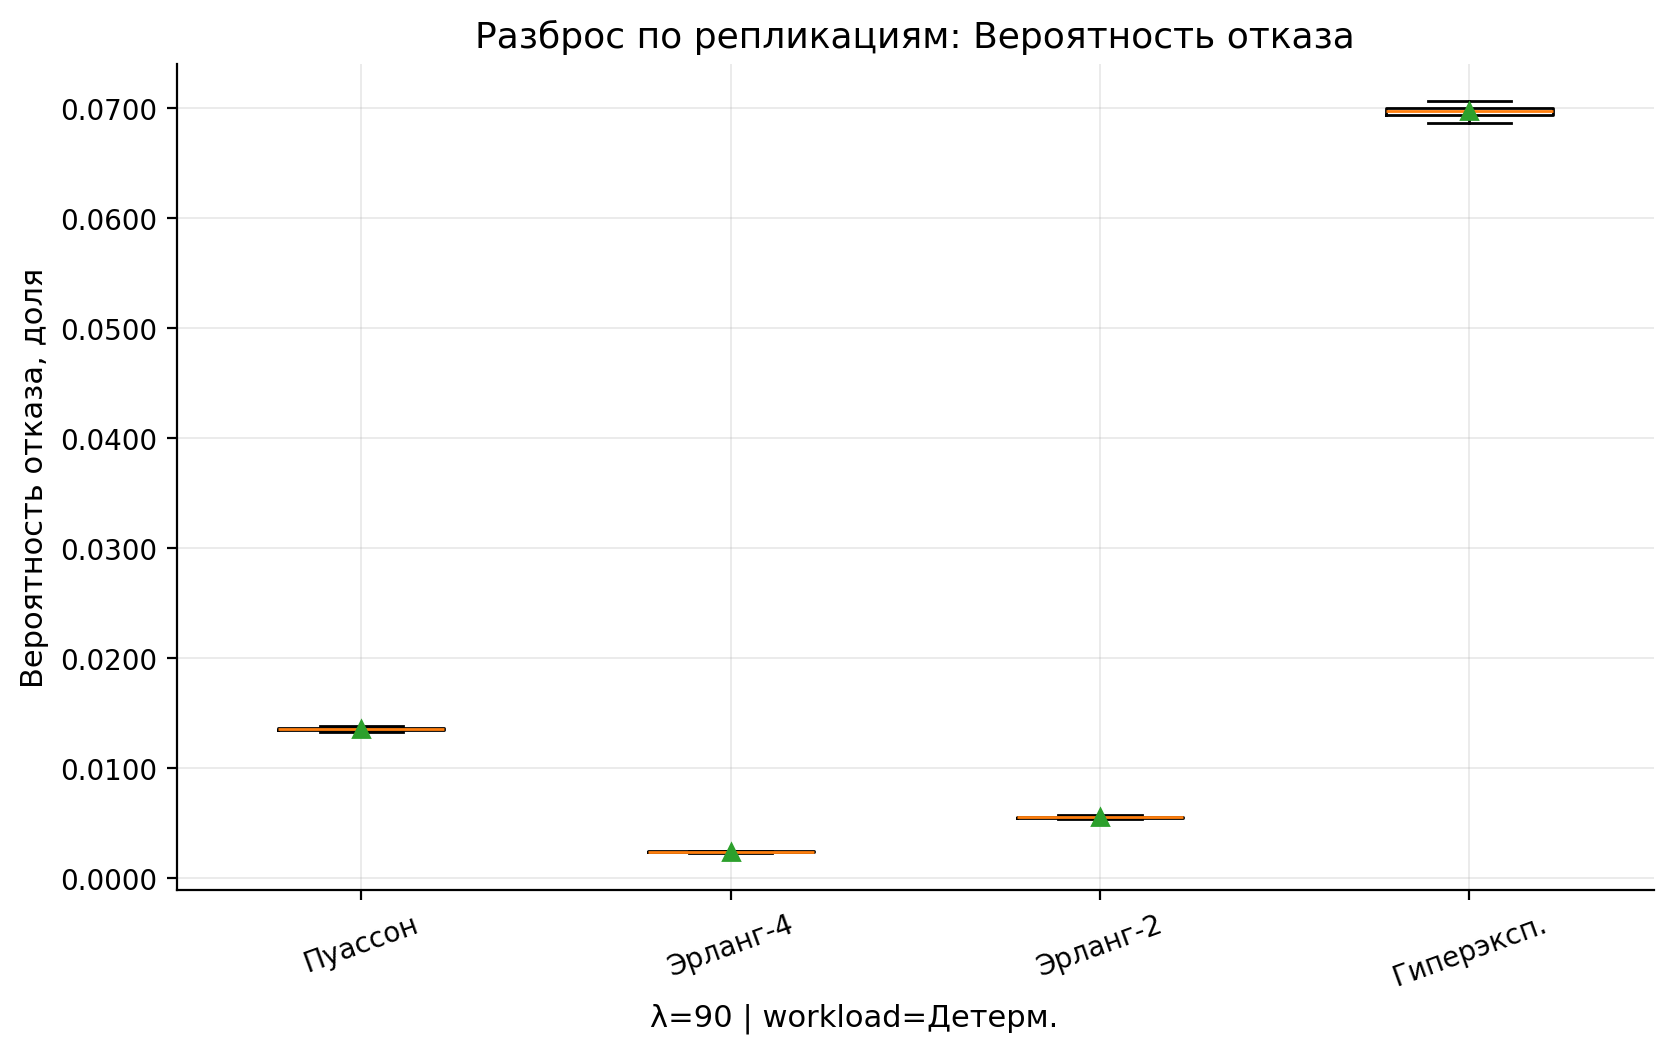
\includegraphics[width=\textwidth]{arrival_sensitivity_boxplot_loss_probability_sigma-1p2_lambda-90.png}
        \caption{Вероятность потери}
    \end{subfigure}
    \hfill
    \begin{subfigure}{0.48\textwidth}
        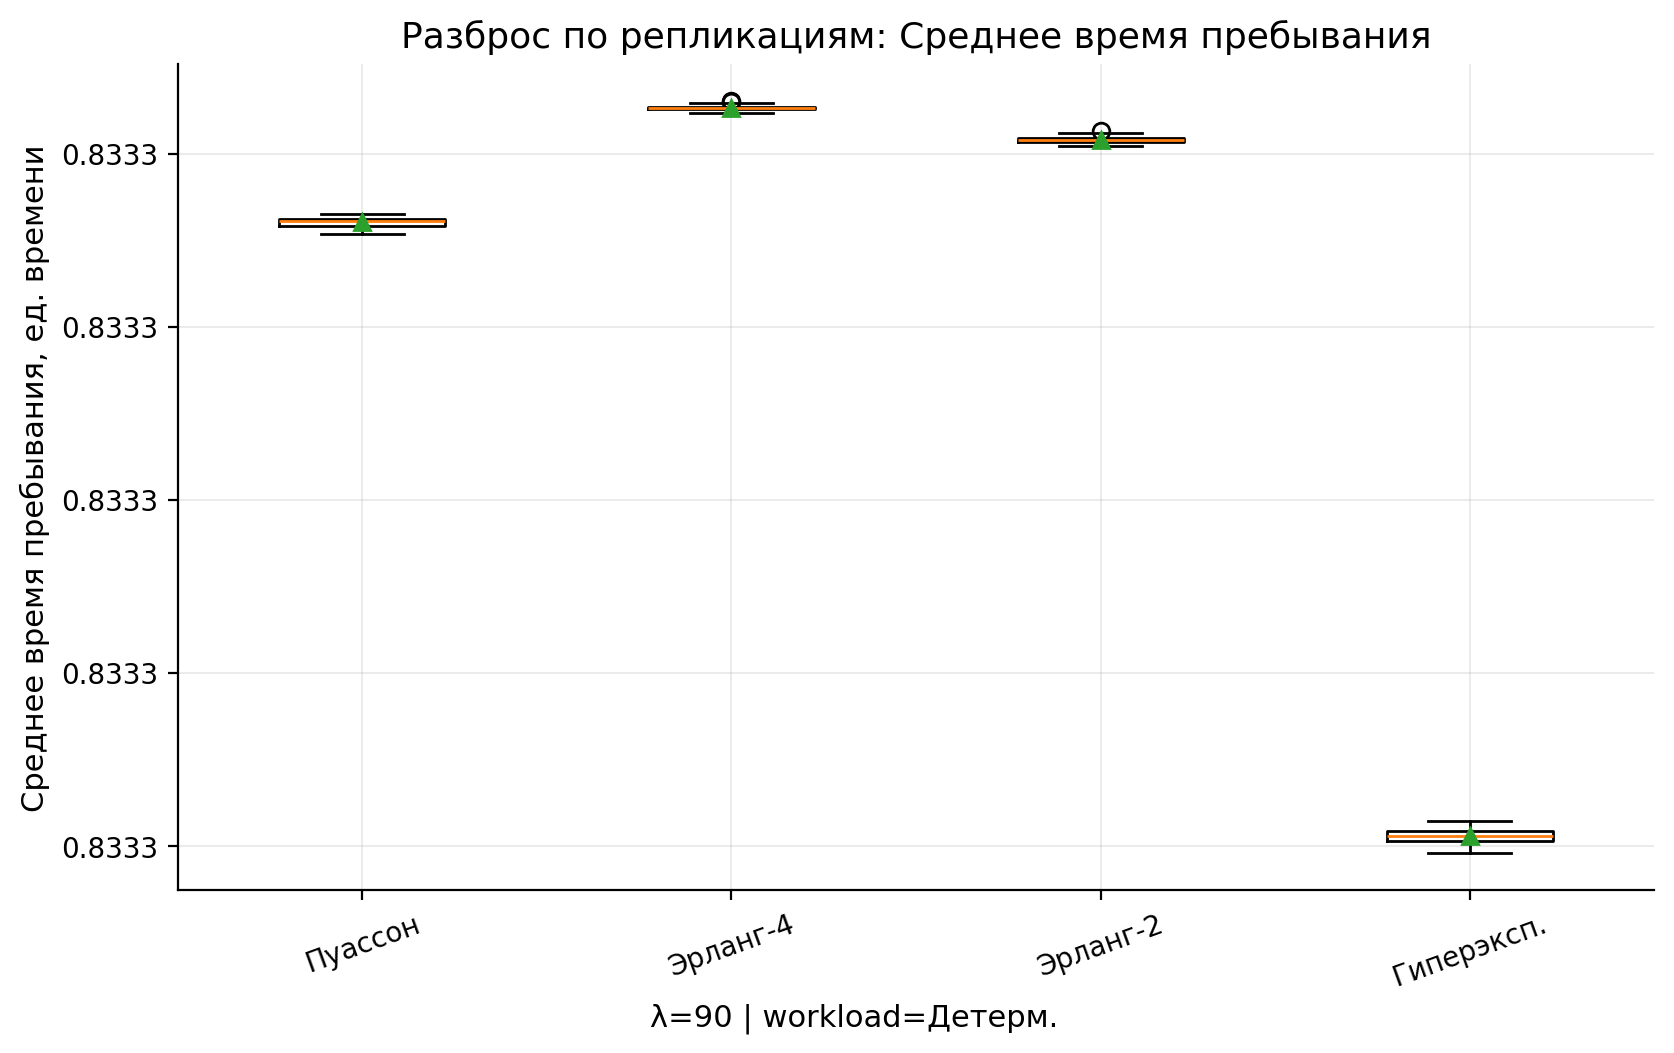
\includegraphics[width=\textwidth]{arrival_sensitivity_boxplot_mean_sojourn_time_sigma-1p2_lambda-90.png}
        \caption{Среднее время пребывания}
    \end{subfigure}
    \caption{Разброс целевых метрик по репликациям в зависимости от типа входящего потока ($\lambda = 90$)}
    \label{fig:app_arrival_boxplots}
\end{figure}

\begin{figure}[H]
    \centering
    \begin{subfigure}{0.48\textwidth}
        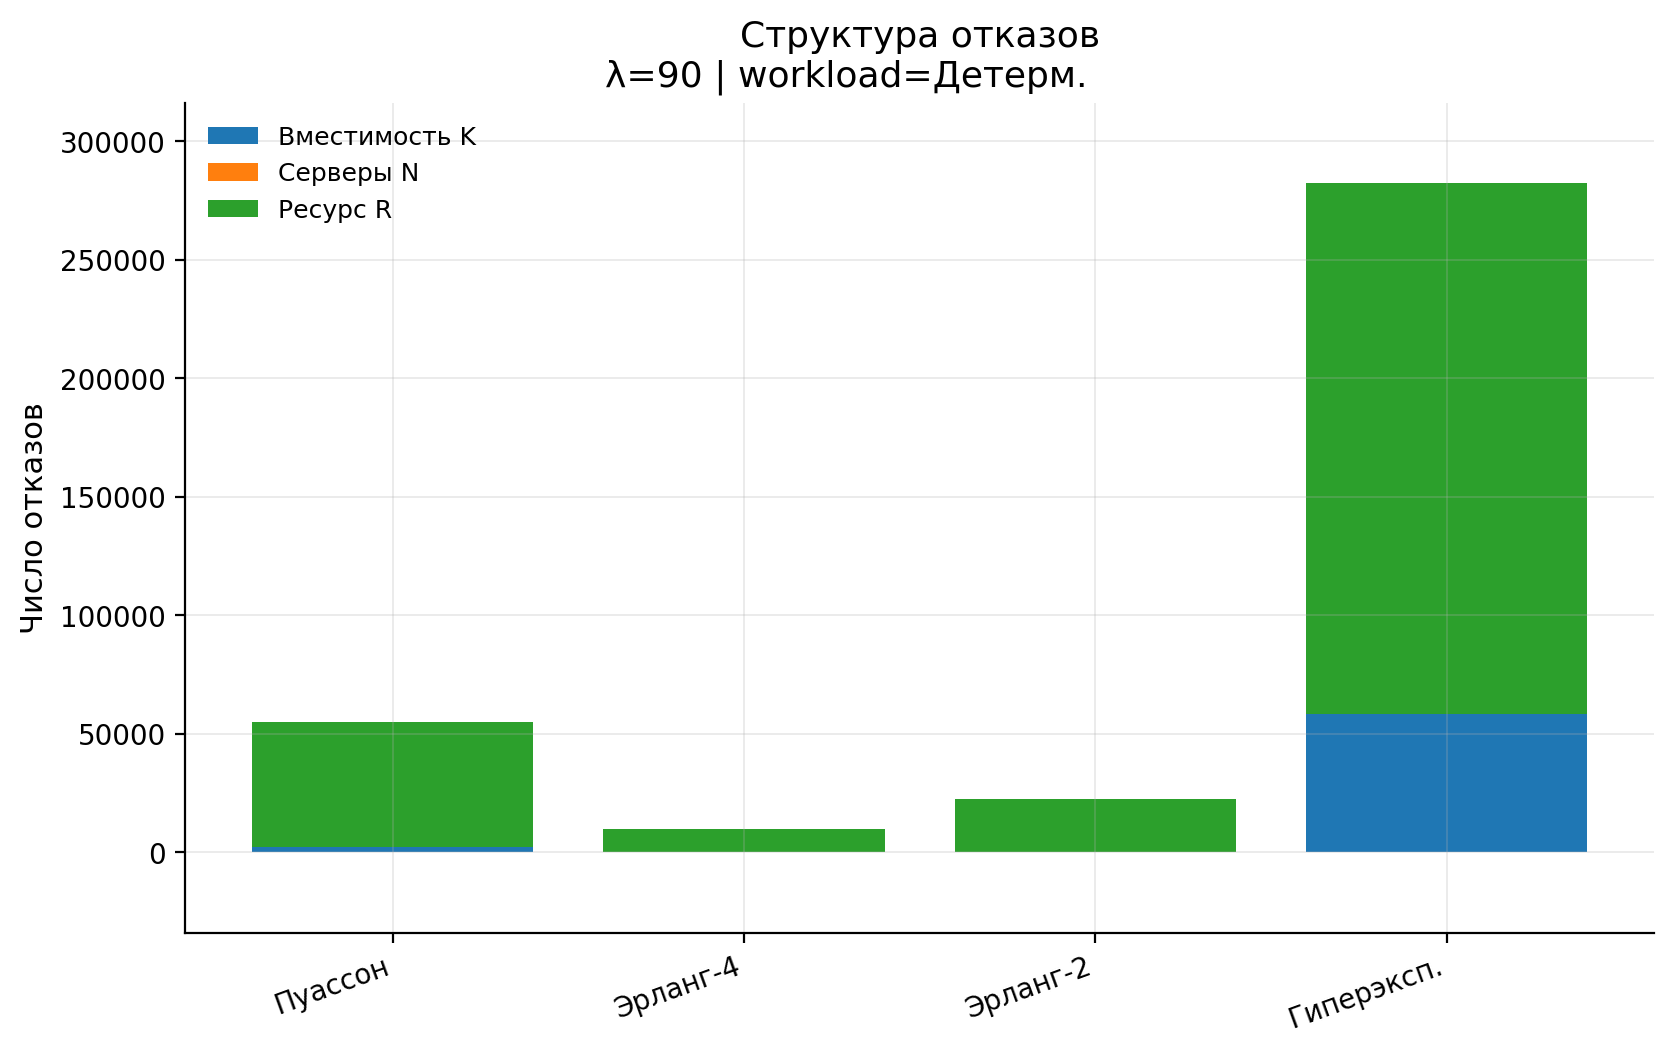
\includegraphics[width=\textwidth]{arrival_sensitivity_rejection_breakdown_sigma-1p2_lambda-90.png}
        \caption{Структура отказов (серверы/ресурс)}
    \end{subfigure}
    \hfill
    \begin{subfigure}{0.48\textwidth}
        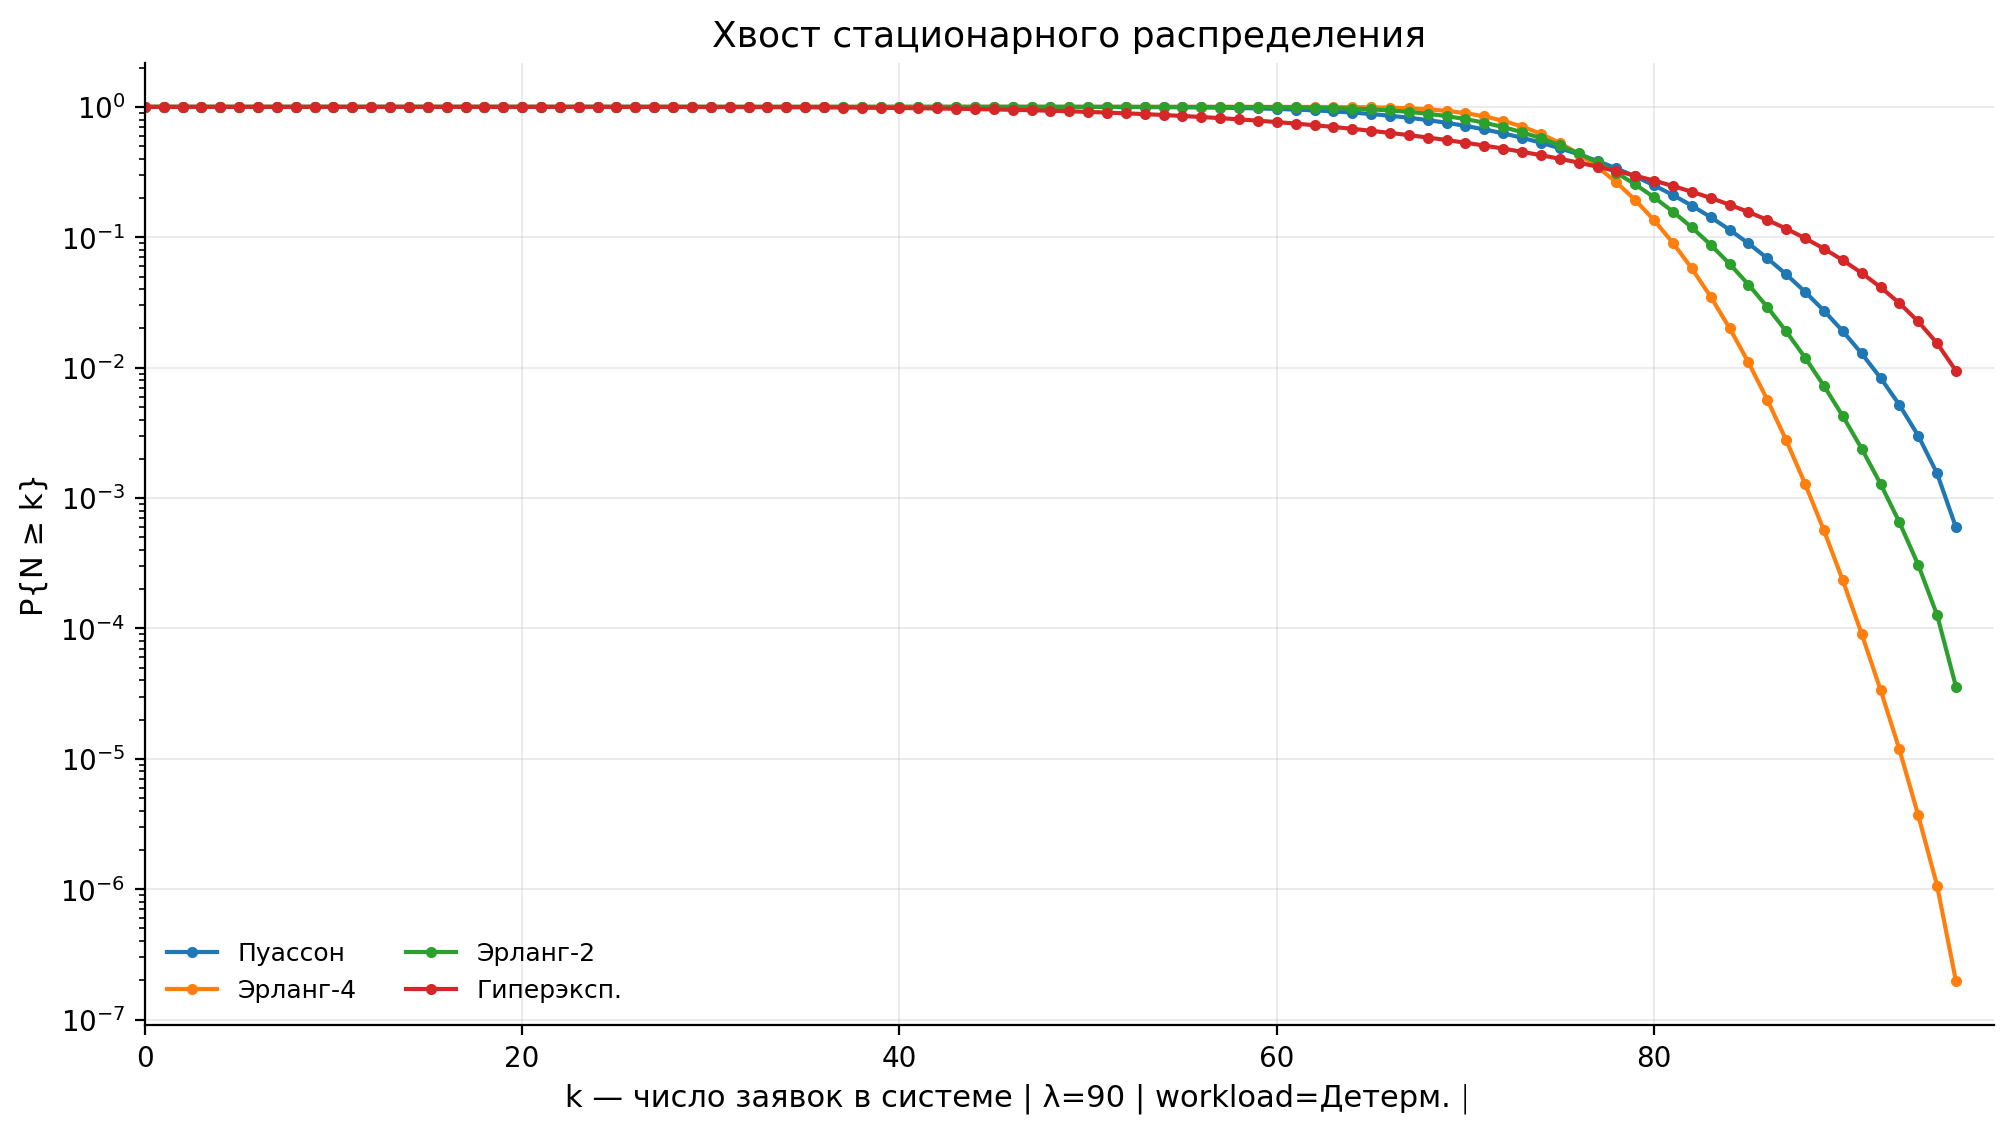
\includegraphics[width=\textwidth]{arrival_sensitivity_stationary_tail_sigma-1p2_lambda-90.png}
        \caption{Хвост стационарного распределения}
    \end{subfigure}
    \caption{Дополнительные метрики чувствительности к входящему потоку ($\lambda = 90$)}
    \label{fig:app_arrival_misc}
\end{figure}


\clearpage
\section{Дополнительные графики совместной чувствительности}
\label{app:combined_plots}

В данном разделе приведены дополнительные тепловые карты и графики относительных отклонений (delta) для тех метрик эффективности, которые не вошли в основной текст третьей главы.

\begin{figure}[H]
    \centering
    \begin{subfigure}{0.48\textwidth}
        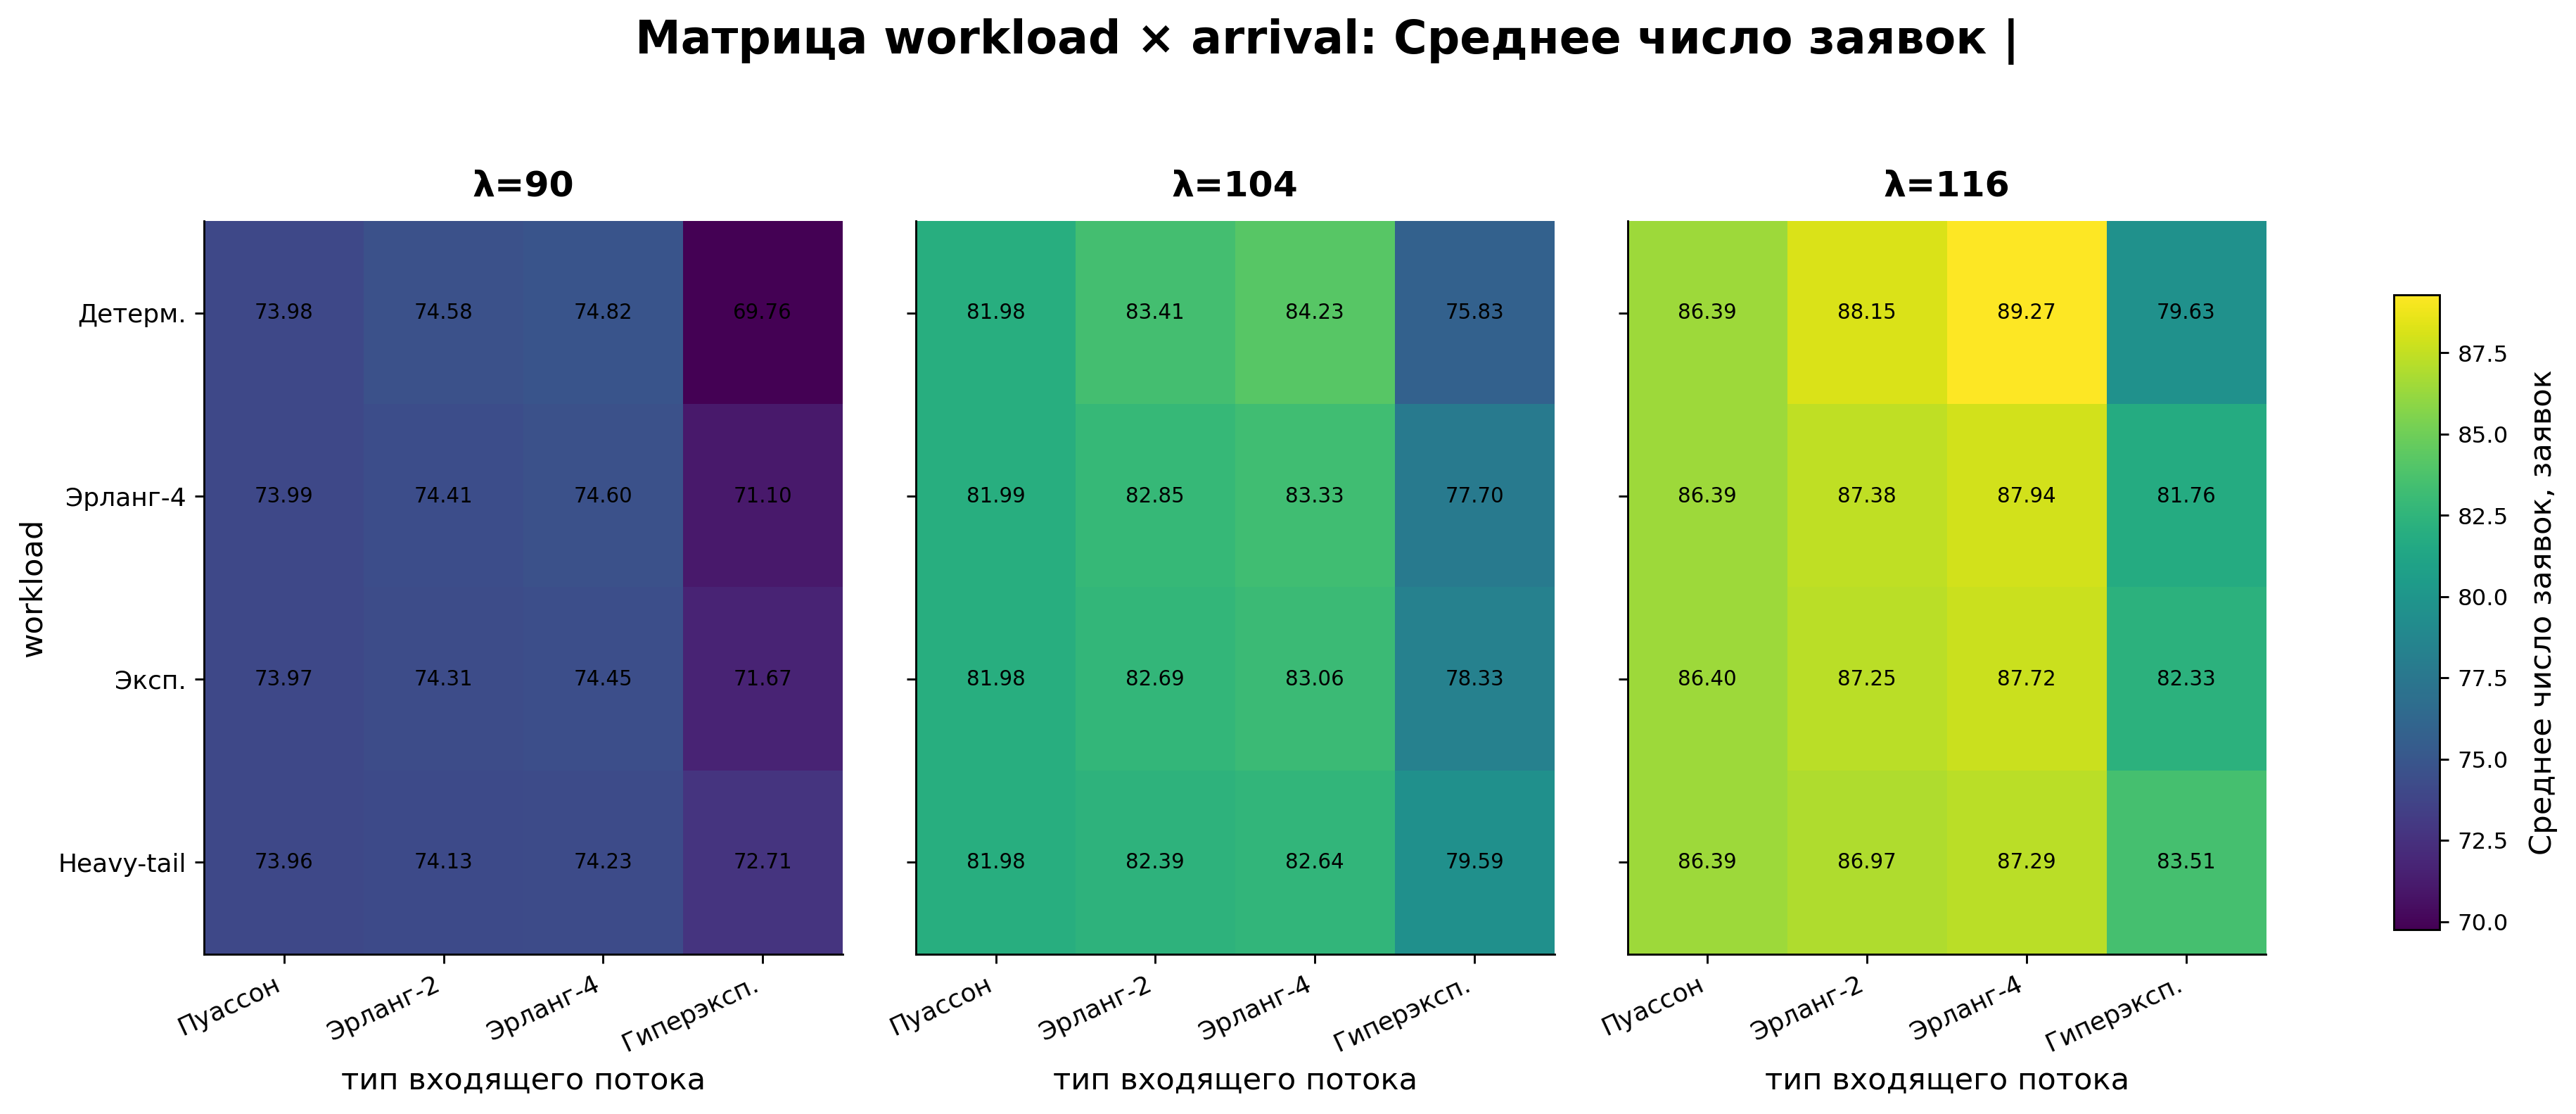
\includegraphics[width=\textwidth]{01_heatmap_workload_arrival_mean_num_jobs_sigma-1p2.png}
        \caption{Среднее число заявок в системе}
    \end{subfigure}
    \hfill
    \begin{subfigure}{0.48\textwidth}
        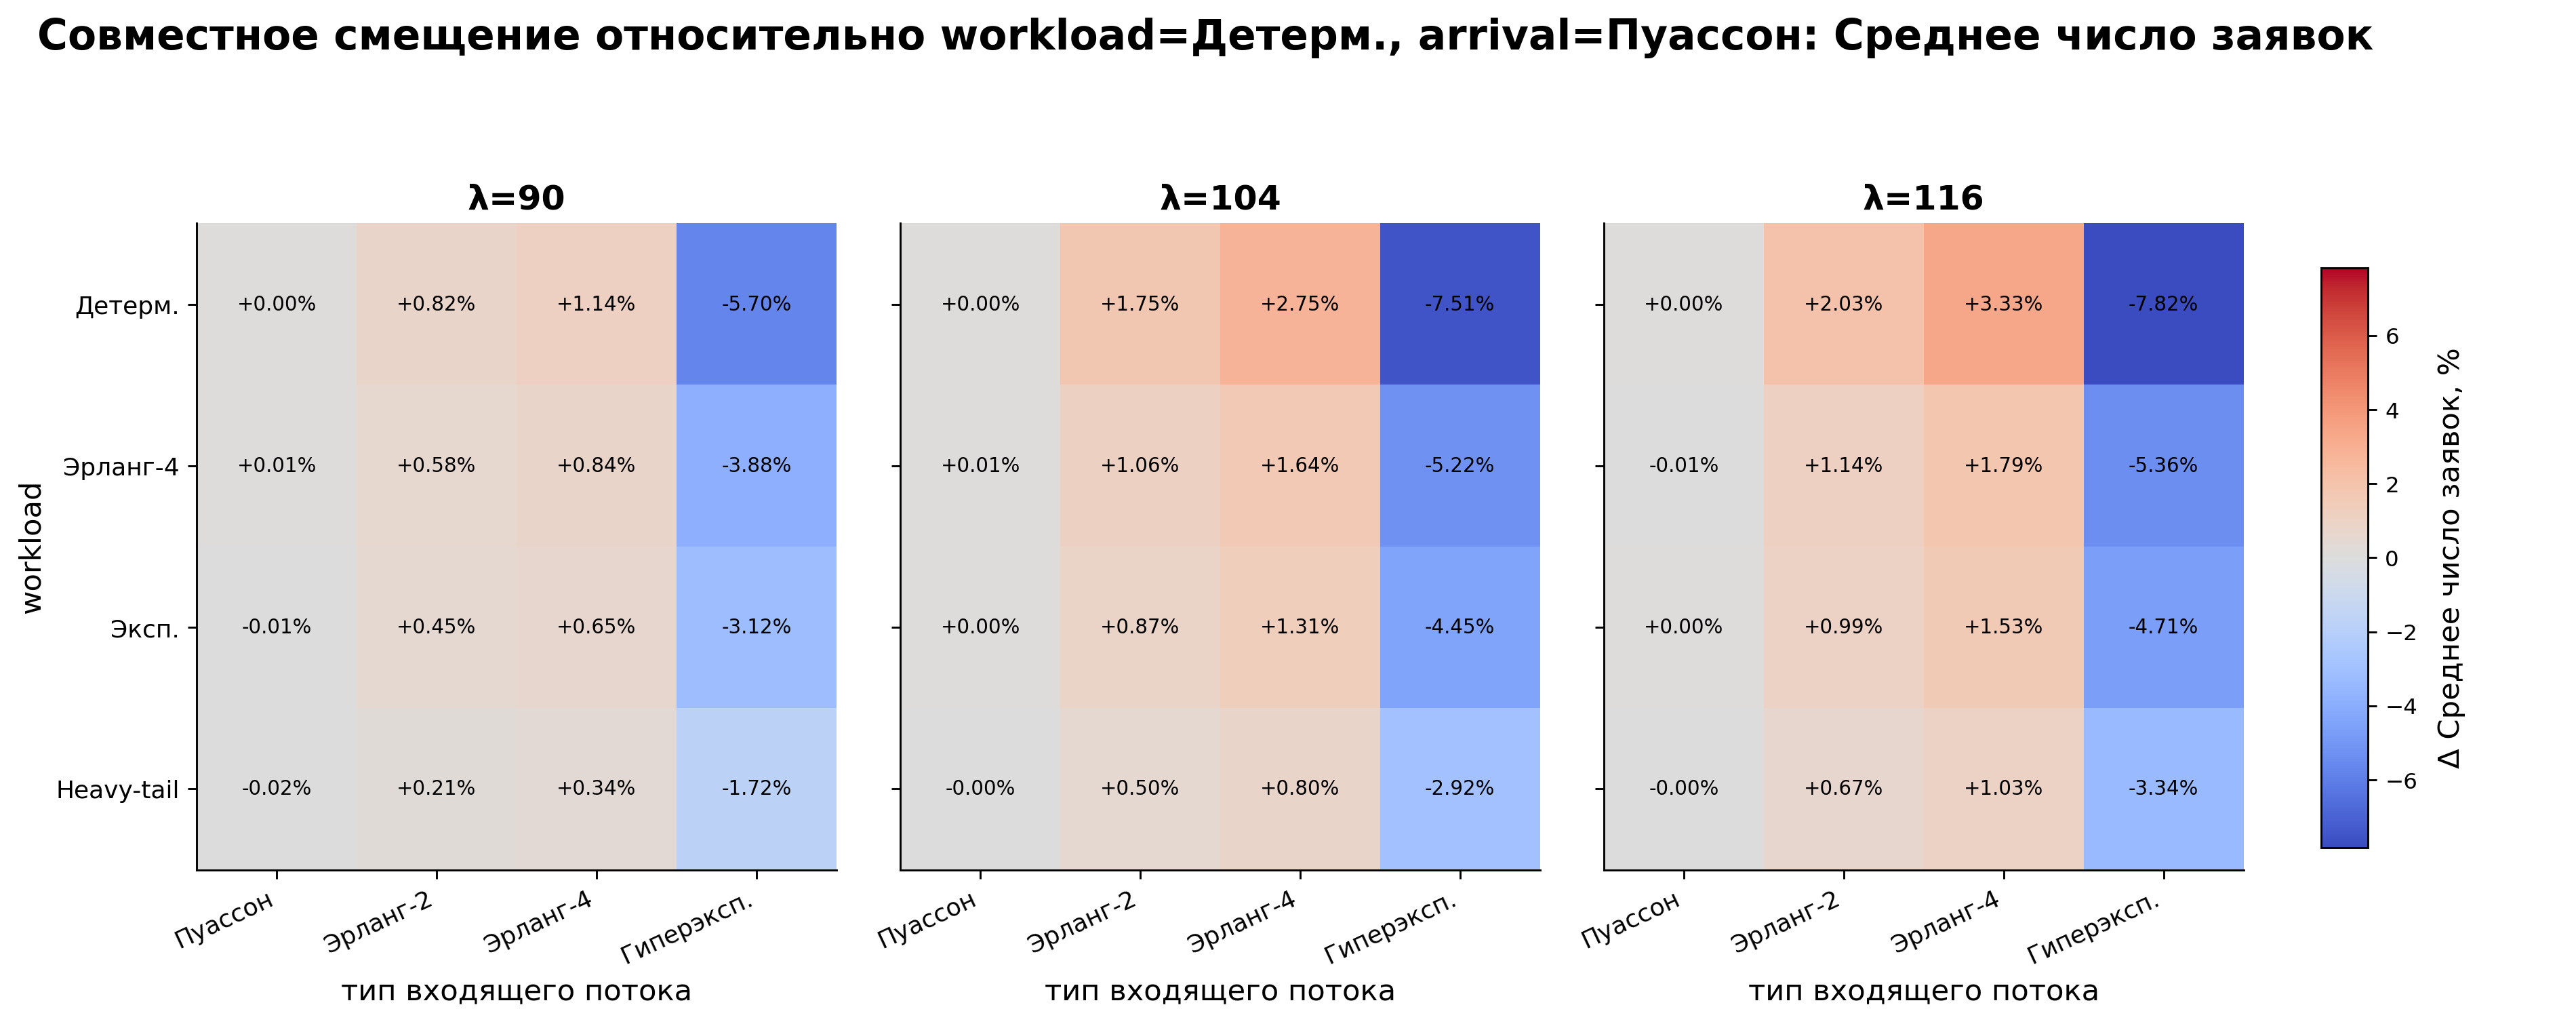
\includegraphics[width=\textwidth]{06_joint_delta_vs_det_poisson_mean_num_jobs_sigma-1p2.png}
        \caption{Смещение числа заявок от базлайна (п.п.)}
    \end{subfigure}
    \caption{Совместное влияние распределений на загруженность системы}
    \label{fig:app_combined_num_jobs}
\end{figure}

На рисунке~\ref{fig:app_combined_compare} показаны срезы чувствительности при фиксации одного из распределений. Левый график демонстрирует изменение метрик при регулярном обслуживании, а правый --- при регулярном входящем потоке заявок.

\begin{figure}[H]
    \centering
    \begin{subfigure}{0.48\textwidth}
        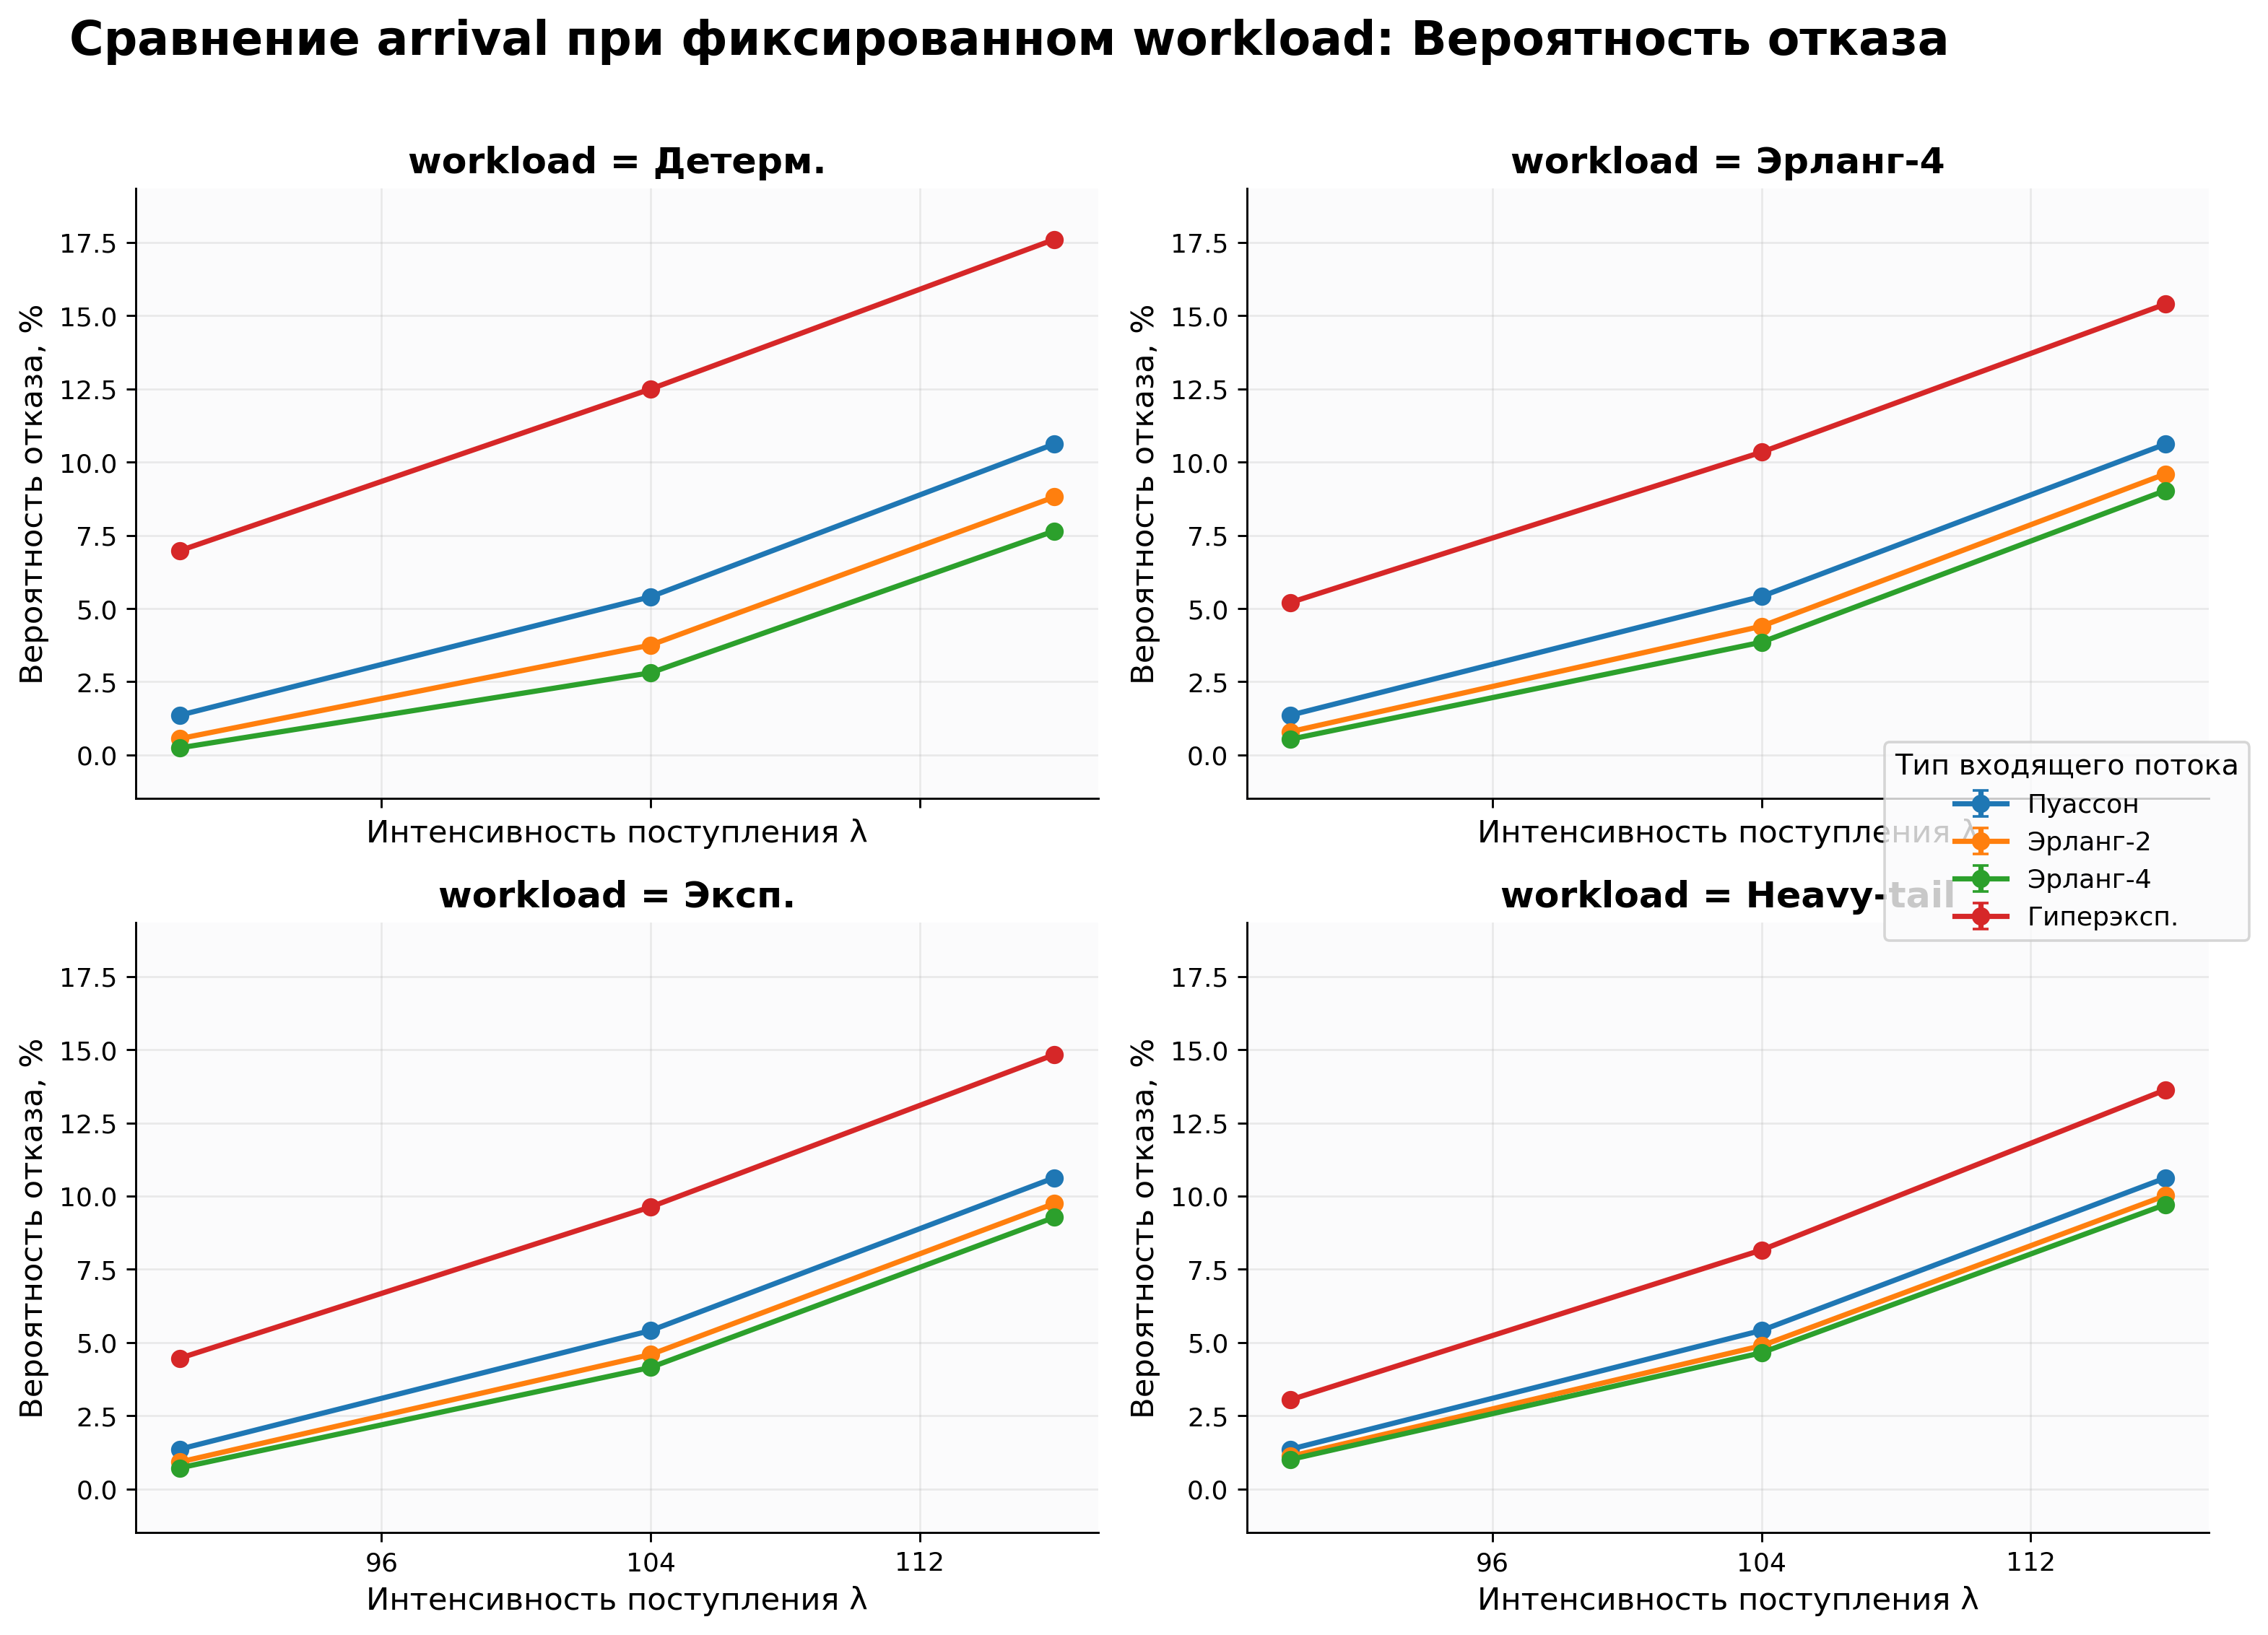
\includegraphics[width=\textwidth]{02_compare_arrivals_fixed_workload_loss_probability_sigma-1p2.png}
        \caption{Сравнение потоков (фиксированный workload)}
    \end{subfigure}
    \hfill
    \begin{subfigure}{0.48\textwidth}
        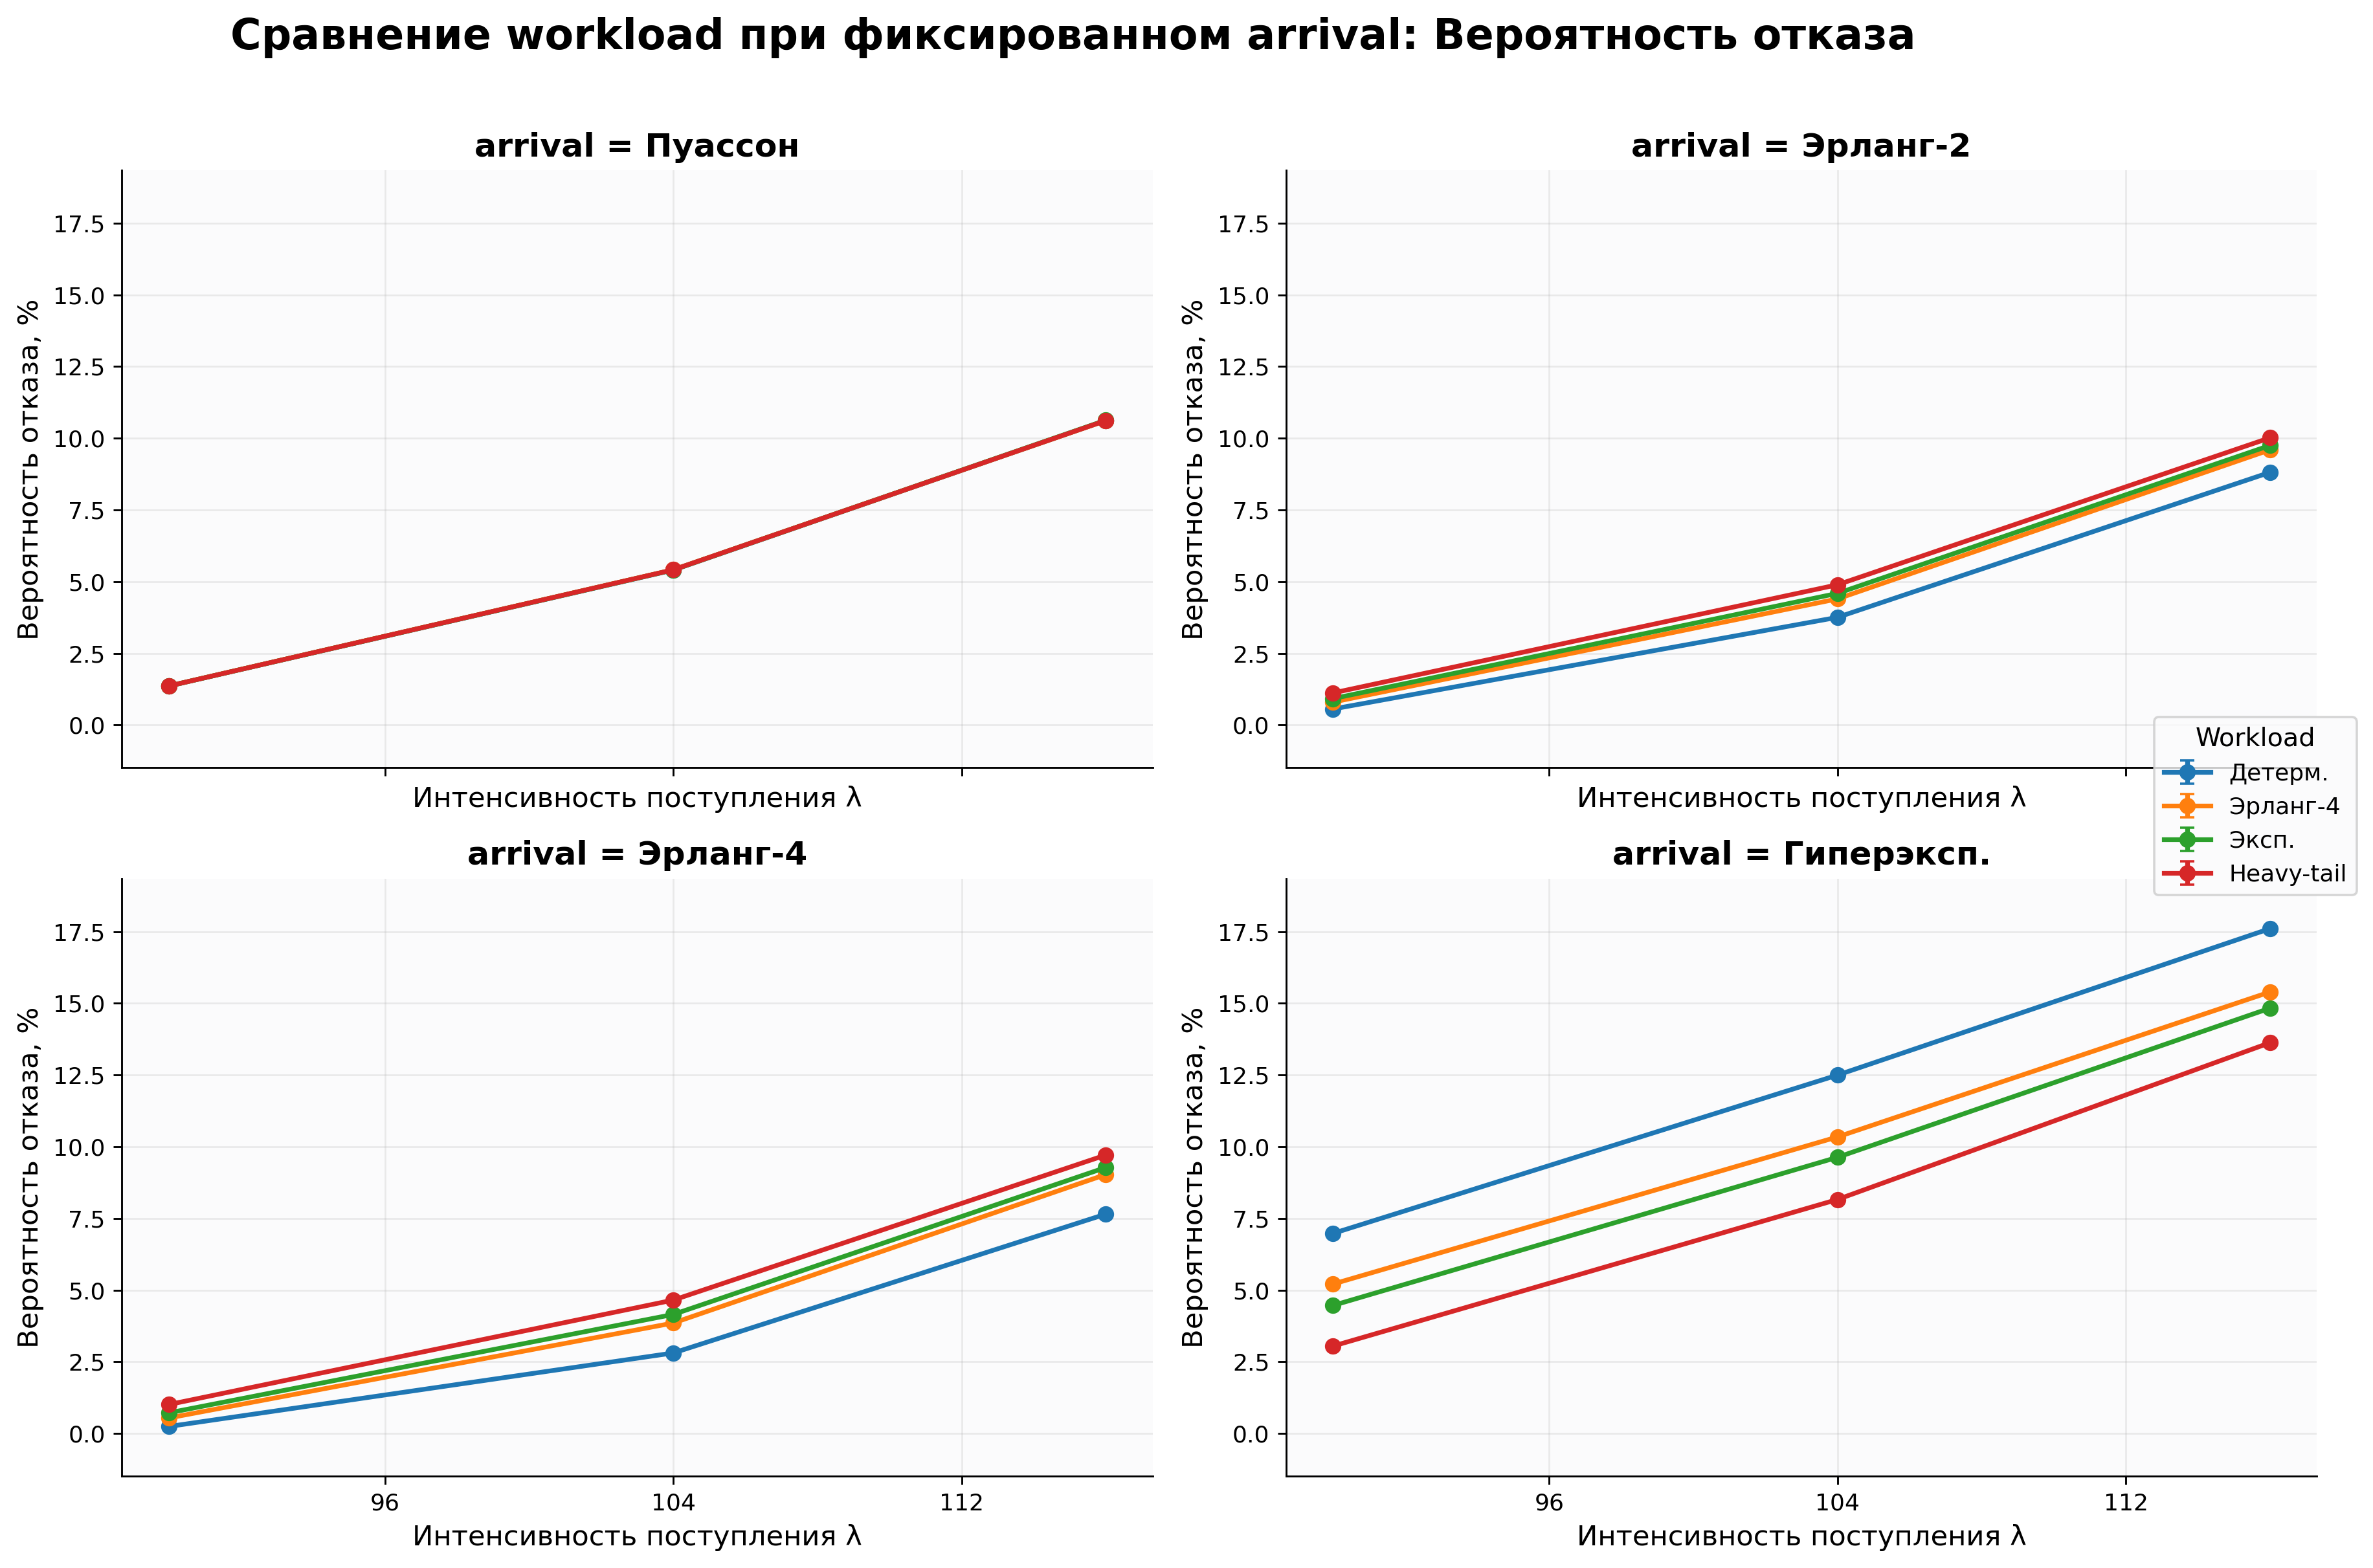
\includegraphics[width=\textwidth]{03_compare_workloads_fixed_arrival_loss_probability_sigma-1p2.png}
        \caption{Сравнение workload (фиксированный поток)}
    \end{subfigure}
    \caption{Срезы совместной чувствительности для вероятности потери}
    \label{fig:app_combined_compare}
\end{figure}

\begin{figure}[H]
    \centering
    \begin{subfigure}{0.48\textwidth}
        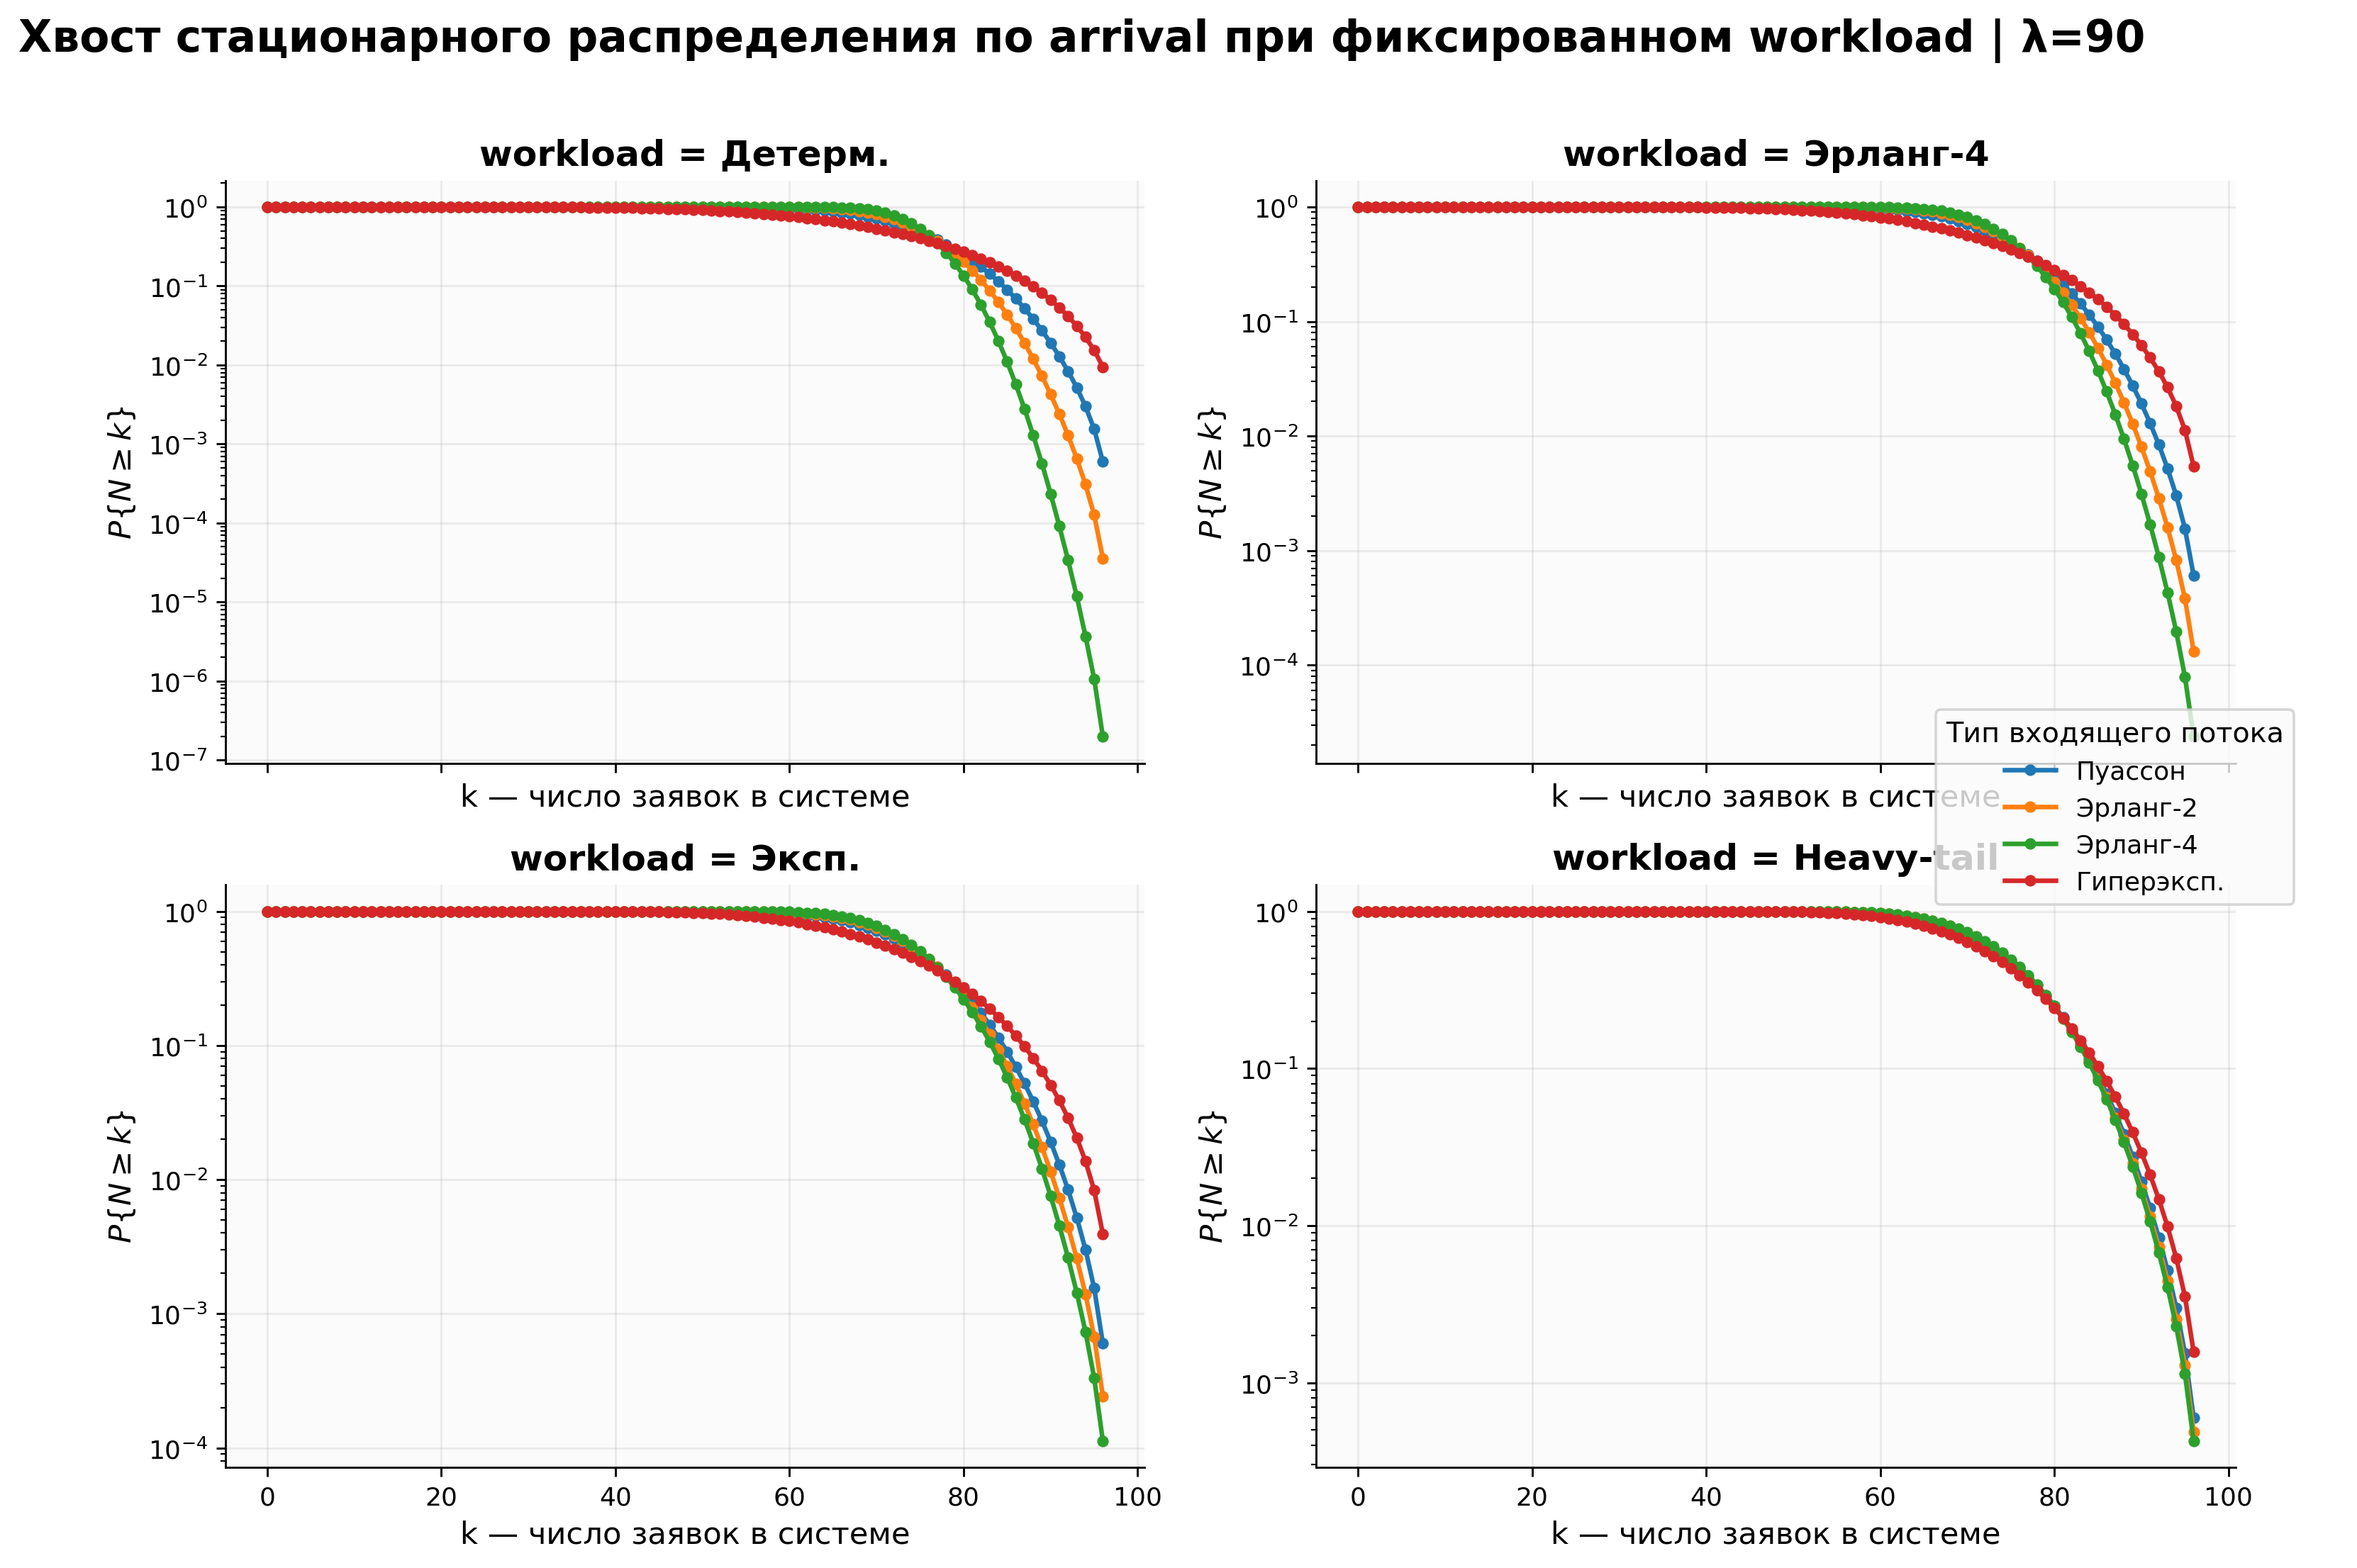
\includegraphics[width=\textwidth]{09_stationary_tail_by_workload_lambda-90_sigma-1p2.png}
        \caption{$\lambda = 90$}
    \end{subfigure}
    \hfill
    \begin{subfigure}{0.48\textwidth}
        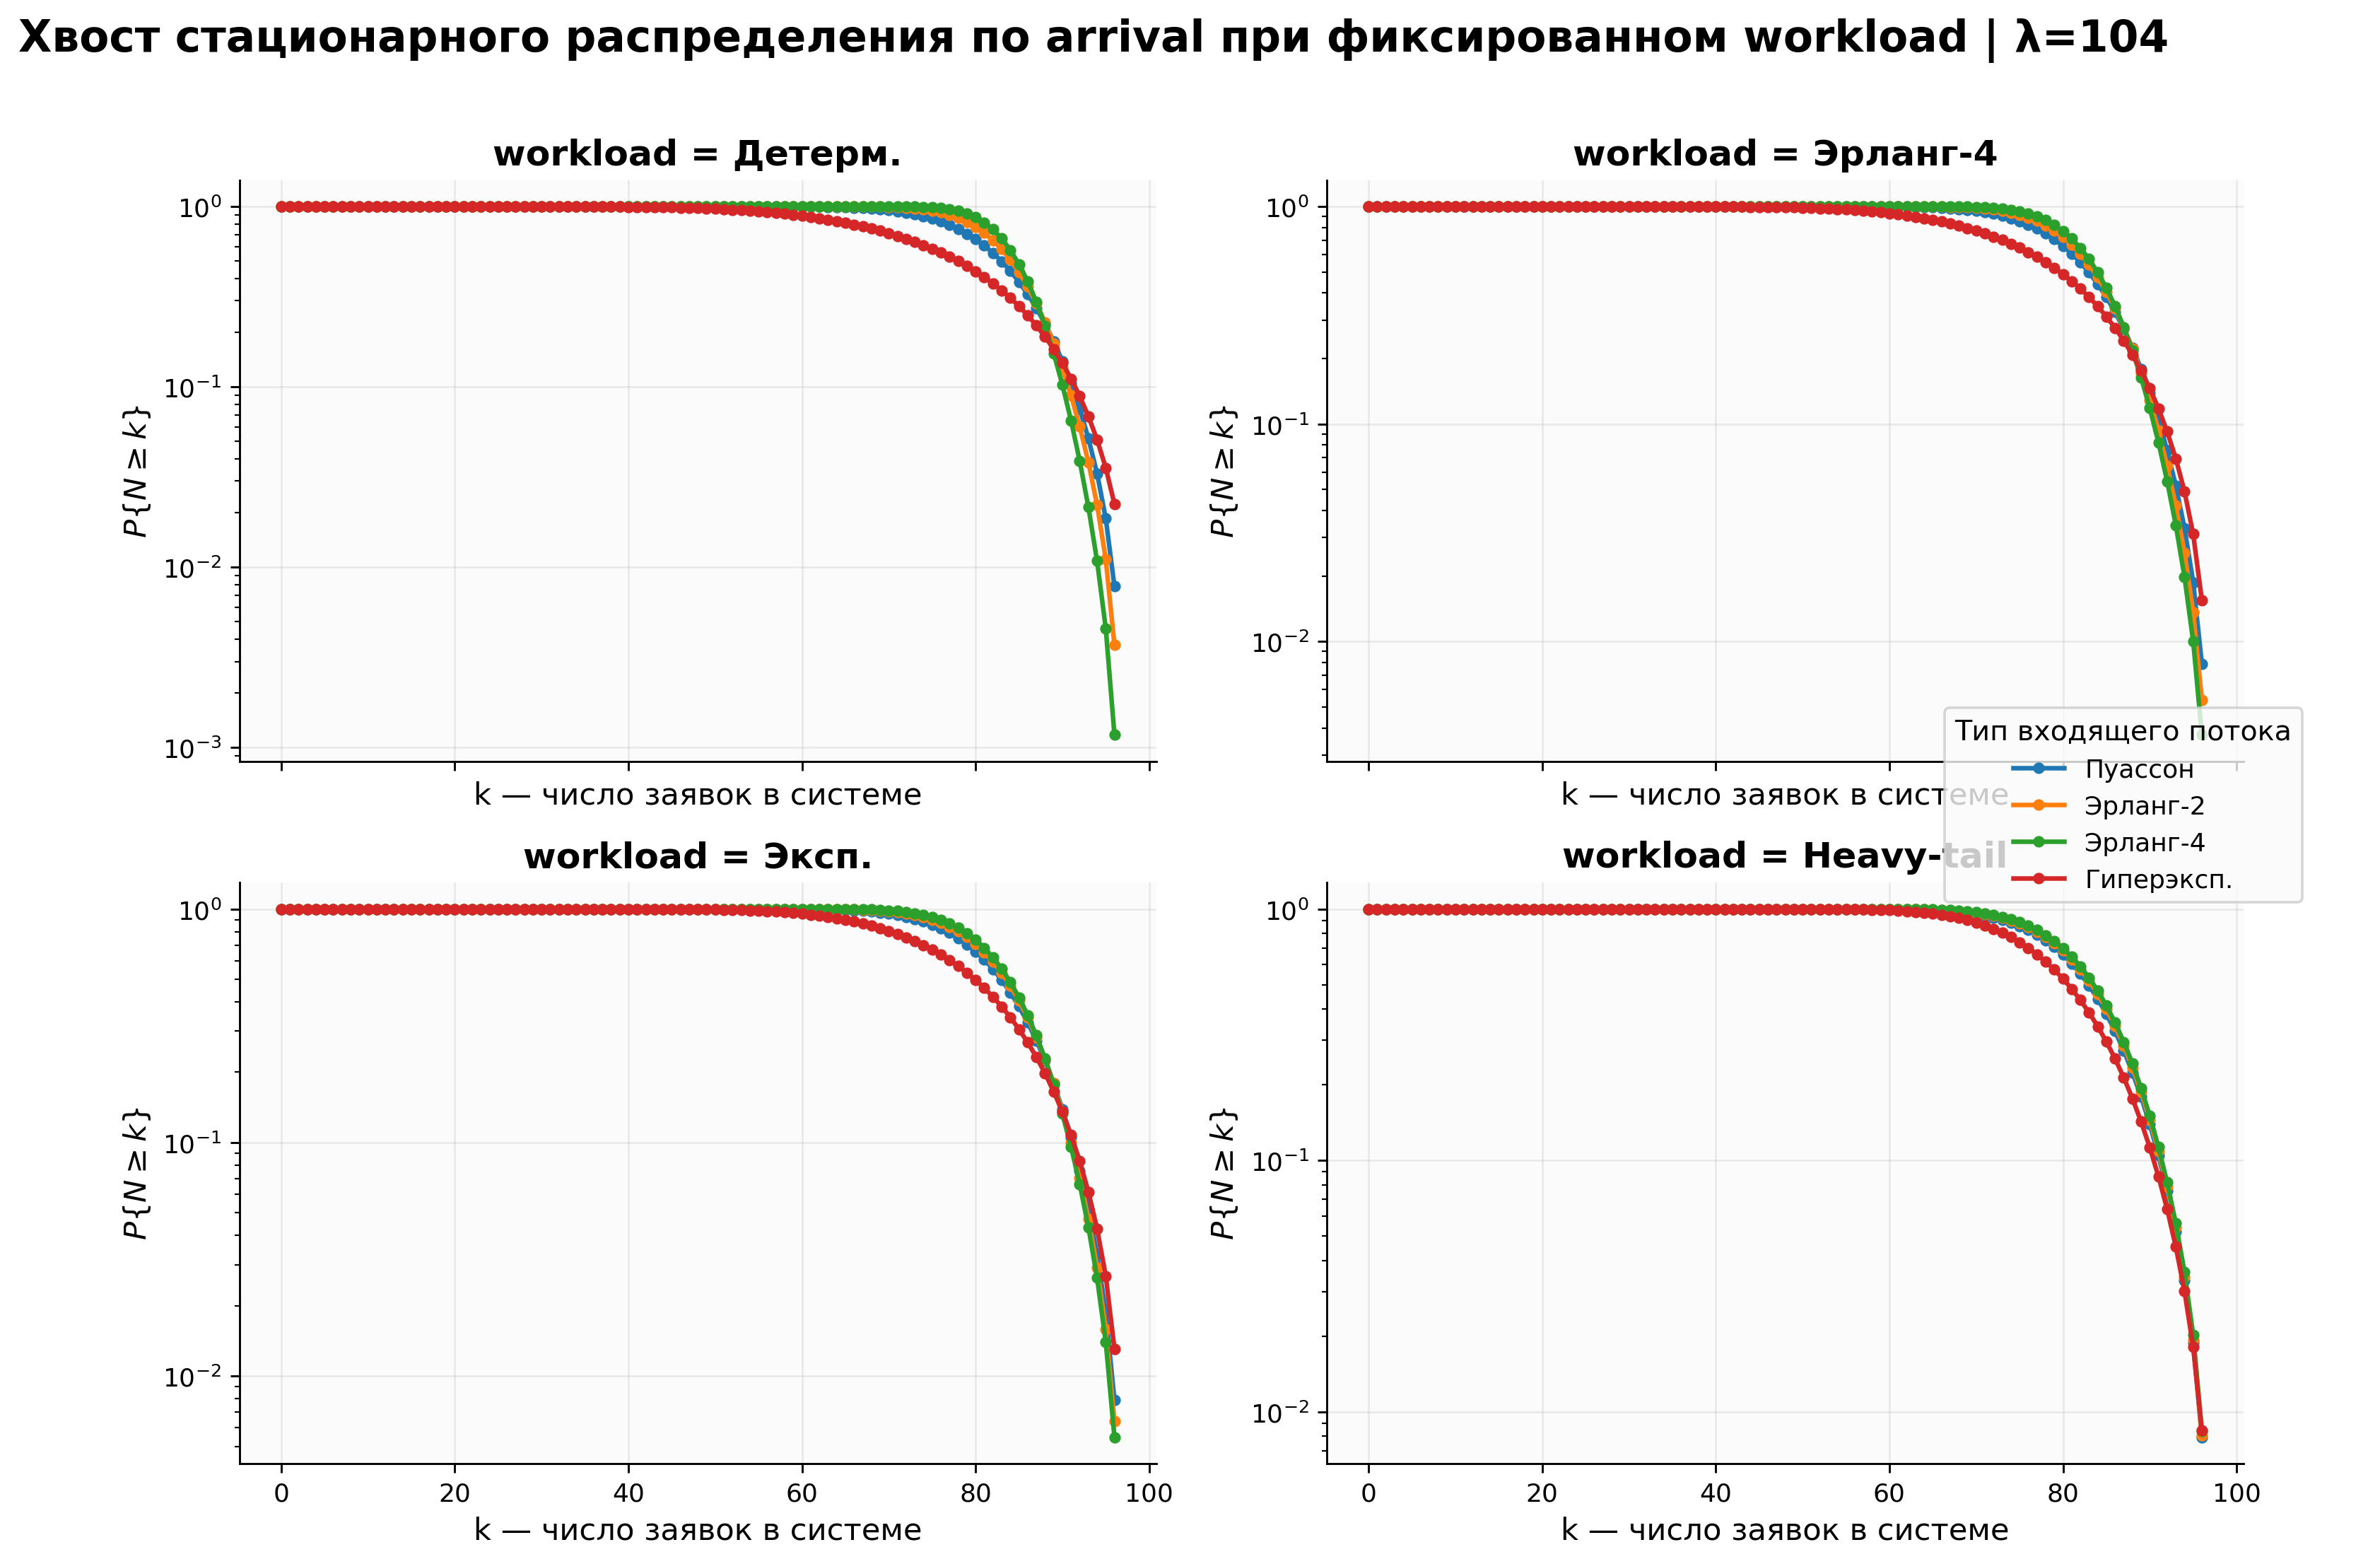
\includegraphics[width=\textwidth]{09_stationary_tail_by_workload_lambda-104_sigma-1p2.png}
        \caption{$\lambda = 104$}
    \end{subfigure}
    \caption{Хвосты стационарных распределений при различных нагрузках в комбинированных сценариях}
    \label{fig:app_combined_tails}
\end{figure}

\end{document}
